\documentclass[12pt]{article}
\usepackage{graphicx} % Required for inserting images
\usepackage{enumitem}
\usepackage[utf8]{inputenc}
\usepackage{amsmath}% For the equation* environment
\usepackage{url}
\usepackage[colorlinks=true, linkcolor=black, citecolor=blue, urlcolor=blue]{hyperref}

\title{Assignment 4 Report}
\author{Mostafa Farrag, Nour Eddine, Youhanna Yousry}
\date{December 2023}

\begin{document}
\maketitle
\newpage
\tableofcontents
\newpage

\section{SSD}
\subsection{Introduction}

\begin{itemize}
    \item SSD, a single-shot detector for multiple categories that is faster than
the previous state-of-the-art for single shot detectors (YOLO), and significantly
more accurate, in fact as accurate as slower techniques that perform explicit region
proposals and pooling (including Faster R-CNN).
    \item The core of SSD is predicting category scores and box offsets for a fixed set of
default bounding boxes using small convolutional filters applied to feature maps.
    \item To achieve high detection accuracy SSD produces predictions of different scales from
feature maps of different scales, and explicitly separate predictions by aspect ratio.
    \item These design features lead to simple end-to-end training and high accuracy, even
on low resolution input images, further improving the speed vs accuracy trade-off.
\end{itemize}

\subsection{Architecture}
\begin{figure}[h]
    \centering
    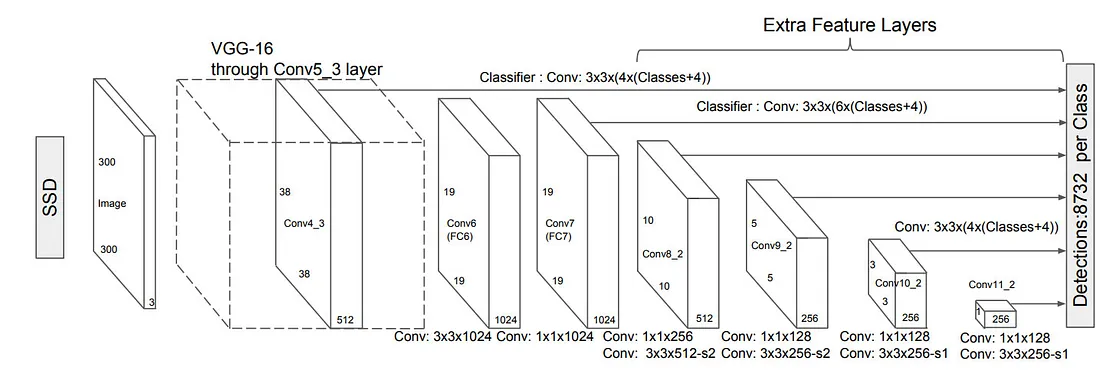
\includegraphics[width=0.75\textwidth]{images/ssd_arch.png}
    \caption{SSD Architecture}
    \label{fig:ssd1}
\end{figure}

The SSD object detection composes of 2 parts:
\begin{enumerate}[leftmargin=1cm, labelwidth=4cm]
  \item Extract feature maps using backbone image classification network.
  \item Apply convolution filters to detect objects.
\end{enumerate}

\begin{figure}[h]
    \centering
    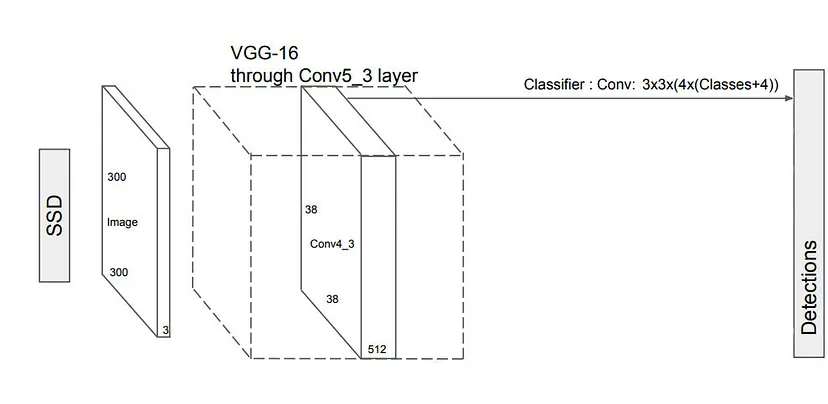
\includegraphics[width=0.75\textwidth]{images/ssd_layer1.png}
    \caption{SSD Layer 1}
    \label{fig:ssd2}
\end{figure}

{
\fontsize{12}{14}\selectfont
SSD uses $VGG16$ to extract feature maps. Then it detects objects using the $Conv_4$ layer. For illustration, we draw the $Conv_4$ to be $8\ X\ 8$ spatially (it should be $38\ X\ 38$). For each cell (also called location), it makes 4 object predictions.
\\
Each prediction composes of a boundary box and 21 scores for each class (one extra class for no object), and we pick the highest score as the class for the bounded object.
\\
$Conv_4$ makes a total of $38\ X\ 38\ X\ 4$ predictions: four predictions per cell regardless of the depth of the feature maps. As expected, many predictions contain no object. SSD reserves a class “0” to indicate it has no objects.
}

\paragraph{Convolutional predictors for object detection}
{
\fontsize{12}{14}\selectfont
SSD does not use a delegated region proposal network. Instead, it resolves to a very simple method. It computes both the location and class scores using small convolution filters. After extracting the feature maps, SSD applies $3\ X\ 3$ convolution filters for each cell to make predictions. (These filters compute the results just like the regular CNN filters.) Each filter outputs 25 channels: 21 scores for each class plus one boundary box (detail on the boundary box later).
}

\paragraph{Multi-scale feature maps for detection}
\begin{figure}[h]
    \centering
    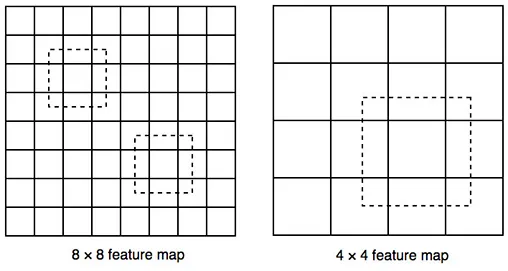
\includegraphics[width=0.75\textwidth]{images/ssd_lh_res.png}
    \caption{SSD Multiscale feature maps}
    \label{fig:ssd3}
\end{figure}
{
\fontsize{12}{14}\selectfont
At first, we describe how SSD detects objects from a single layer. Actually, it uses multiple layers (multi-scale feature maps) to detect objects independently. As CNN reduces the spatial dimension gradually, the resolution of the feature maps also decrease. SSD uses lower resolution layers to detect larger scale objects. For example, the $4\ X\ 4$ feature maps are used for larger scale object.
}

\paragraph{Default boundary box}
{
\fontsize{12}{14}\selectfont
To keep the complexity low, the default boxes are pre-selected manually and carefully to cover a wide spectrum of real-life objects. SSD also keeps the default boxes to a minimum (4 or 6) with one prediction per default box. Now, instead of using global coordination for the box location, the boundary box predictions are relative to the default boundary boxes at each cell $(\Delta cx, \Delta cy, \Delta w, \Delta h)$, i.e. the offsets (difference) to the default box at each cell for its center $(cx, cy)$, the width and the height.
\\
For each feature map layers, it shares the same set of default boxes centered at the corresponding cell. But different layers use different sets of default boxes to customize object detections at different resolutions.
}

\paragraph{Multi-scale feature maps \& Default boundary boxes}
\begin{figure}[h]
    \centering
    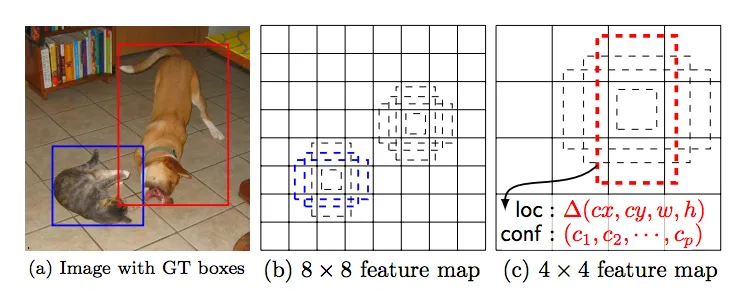
\includegraphics[width=0.75\textwidth]{images/ssd_cat_dog.png}
    \caption{Detecting at different scales}
    \label{fig:ssd4}
\end{figure}
{
\fontsize{12}{14}\selectfont
Here is an example of how SSD combines multi-scale feature maps and default boundary boxes to detect objects at different scales and aspect ratios. The dog below matches one default box (in red) in the $4\ X\ 4$ feature map layer, but not any default boxes in the higher resolution $8\ X\ 8$ feature map. The cat which is smaller is detected only by the $8\ X\ 8$ feature map layer in 2 default boxes (in blue).
}

\subsection{Inference Results}

\begin{figure}[htbp]
    {\raggedright
    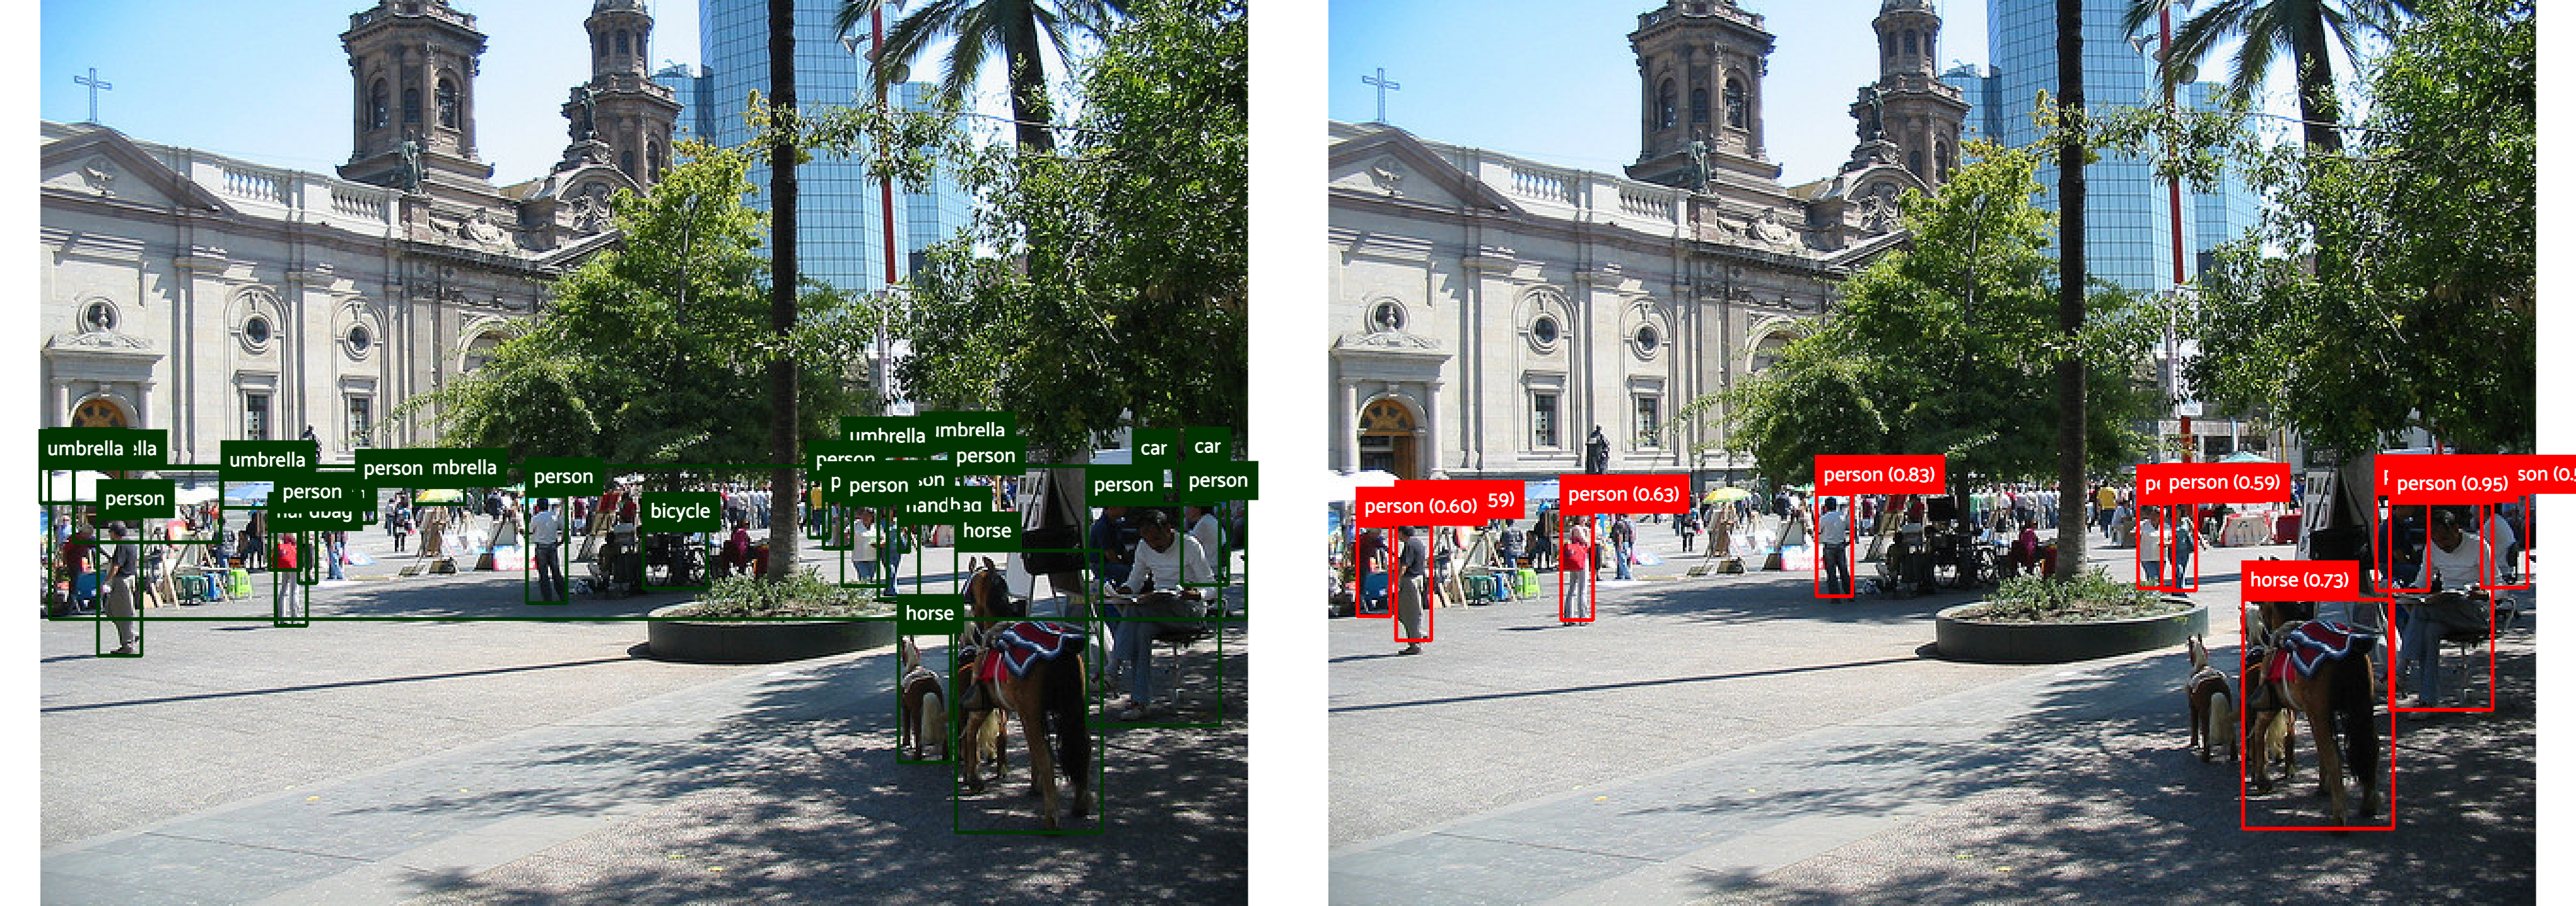
\includegraphics[width=0.5\textwidth]{images/ssd_res/ssd_b1.png}
    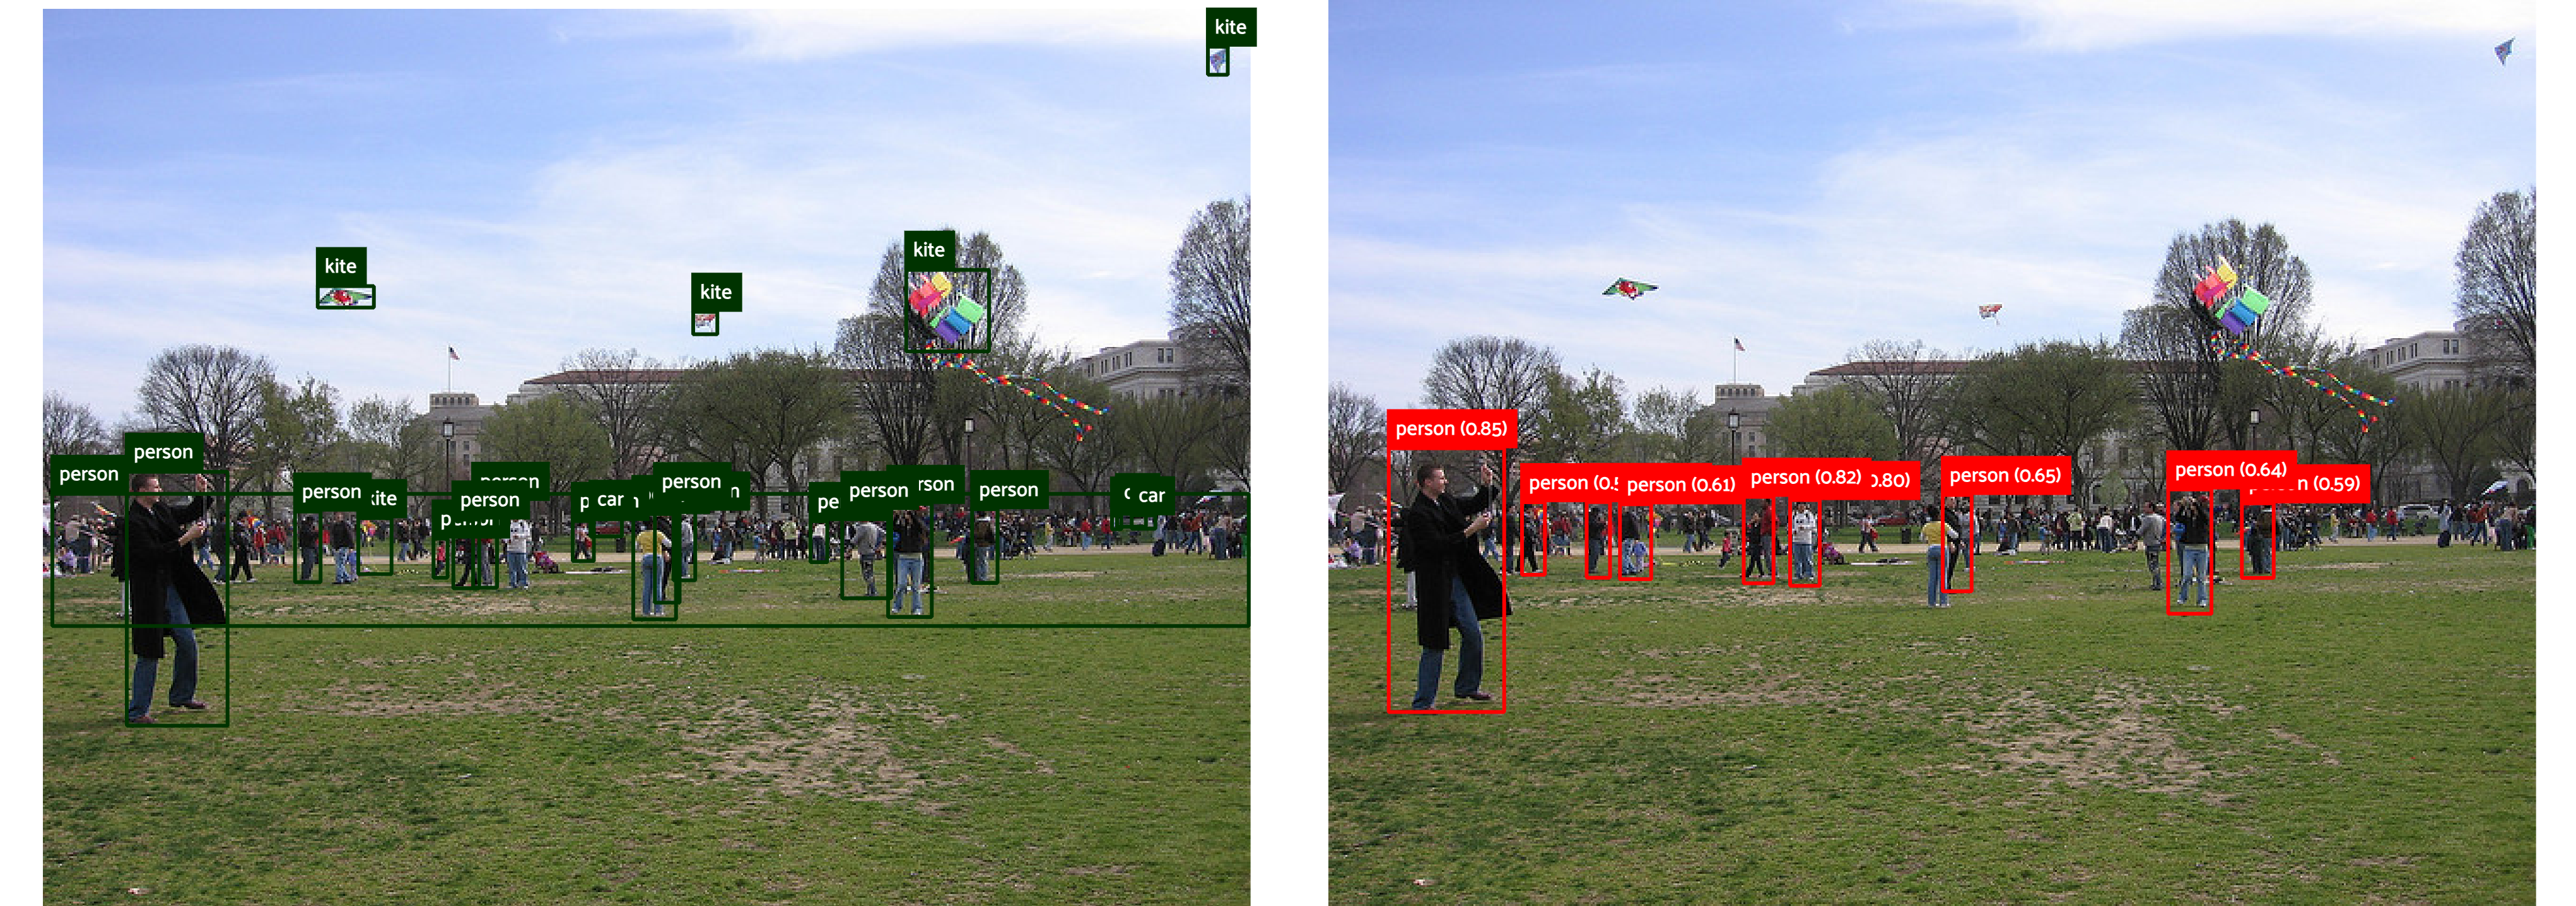
\includegraphics[width=0.5\textwidth]{images/ssd_res/ssd_b2.png}
    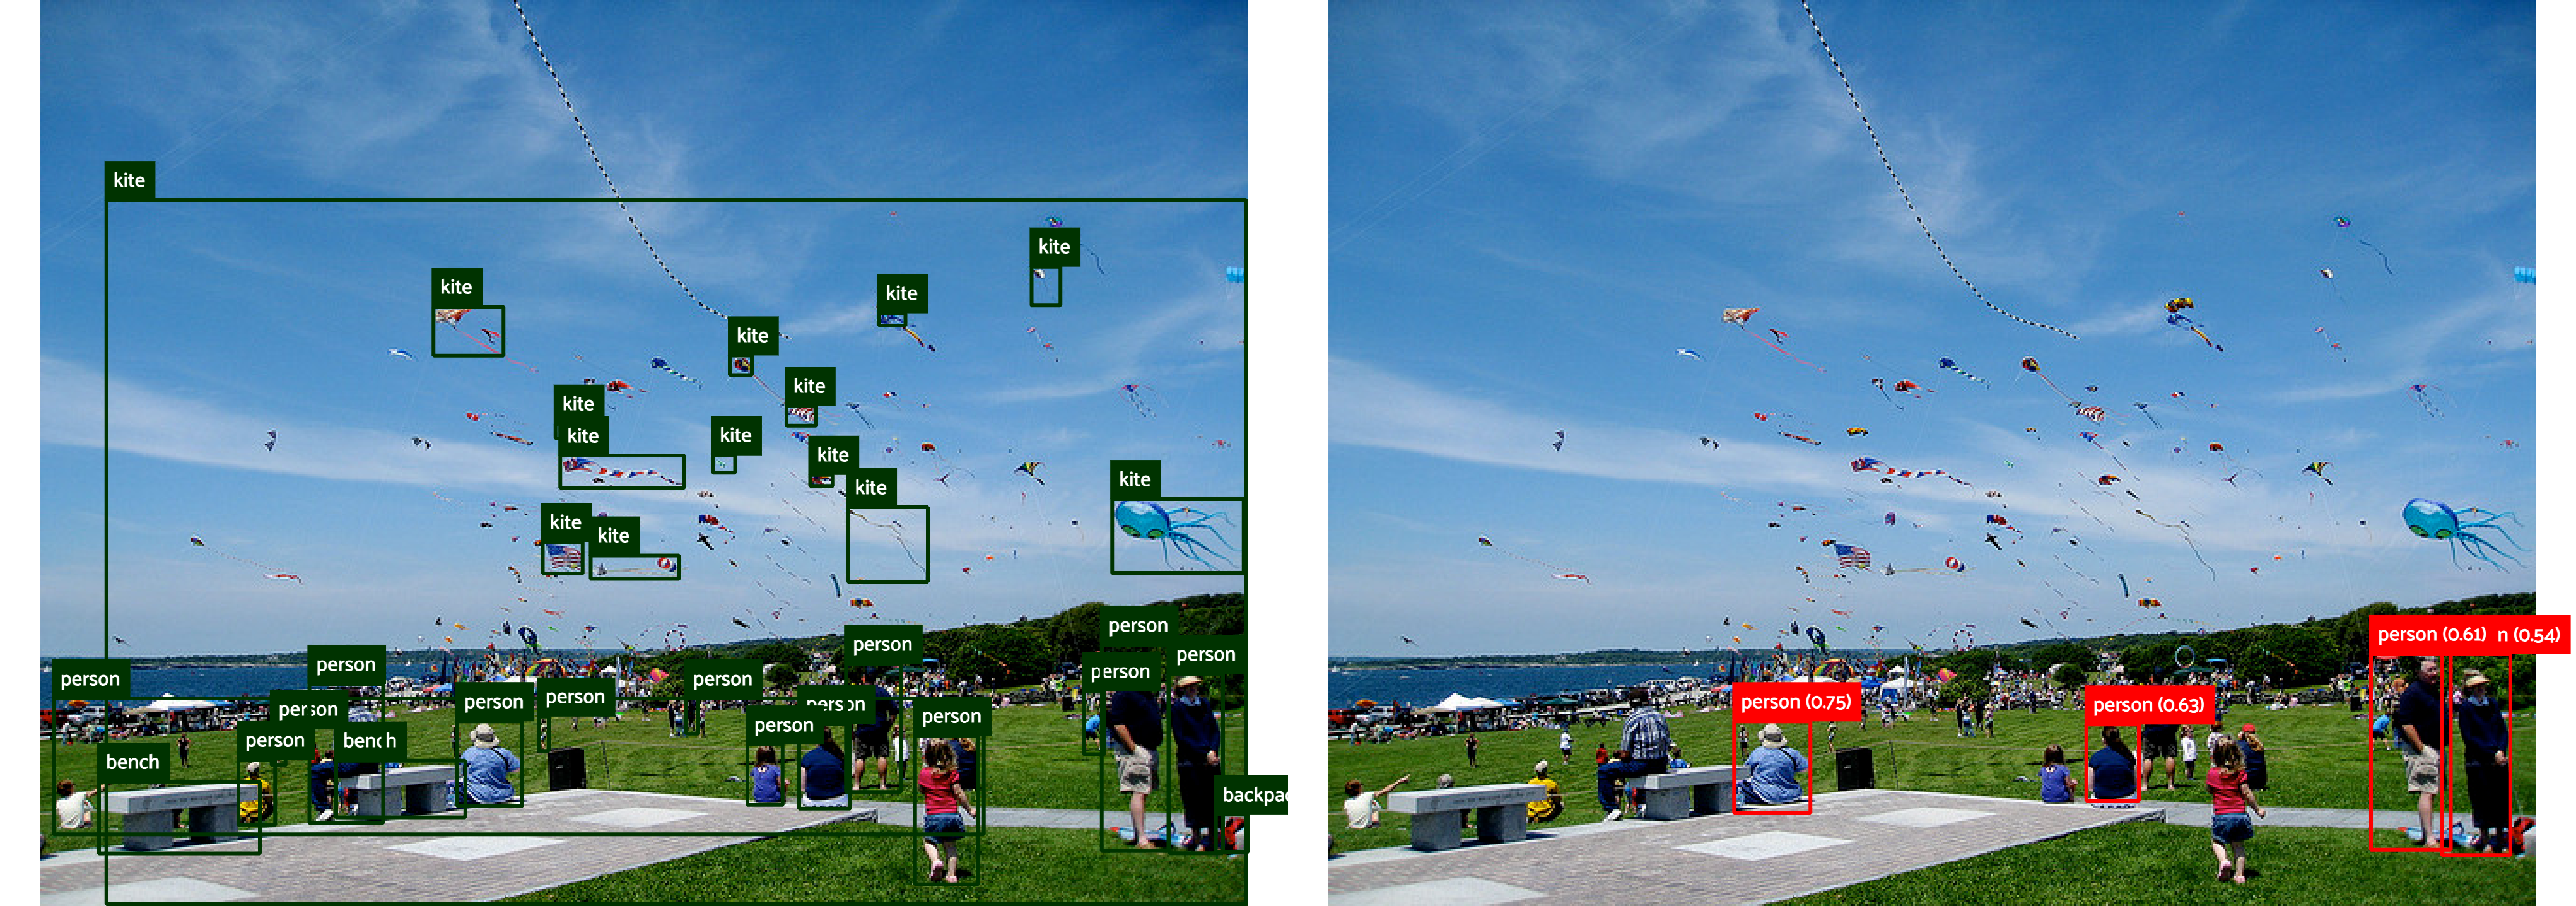
\includegraphics[width=0.5\textwidth]{images/ssd_res/ssd_b3.png}}
    {\raggedleft
    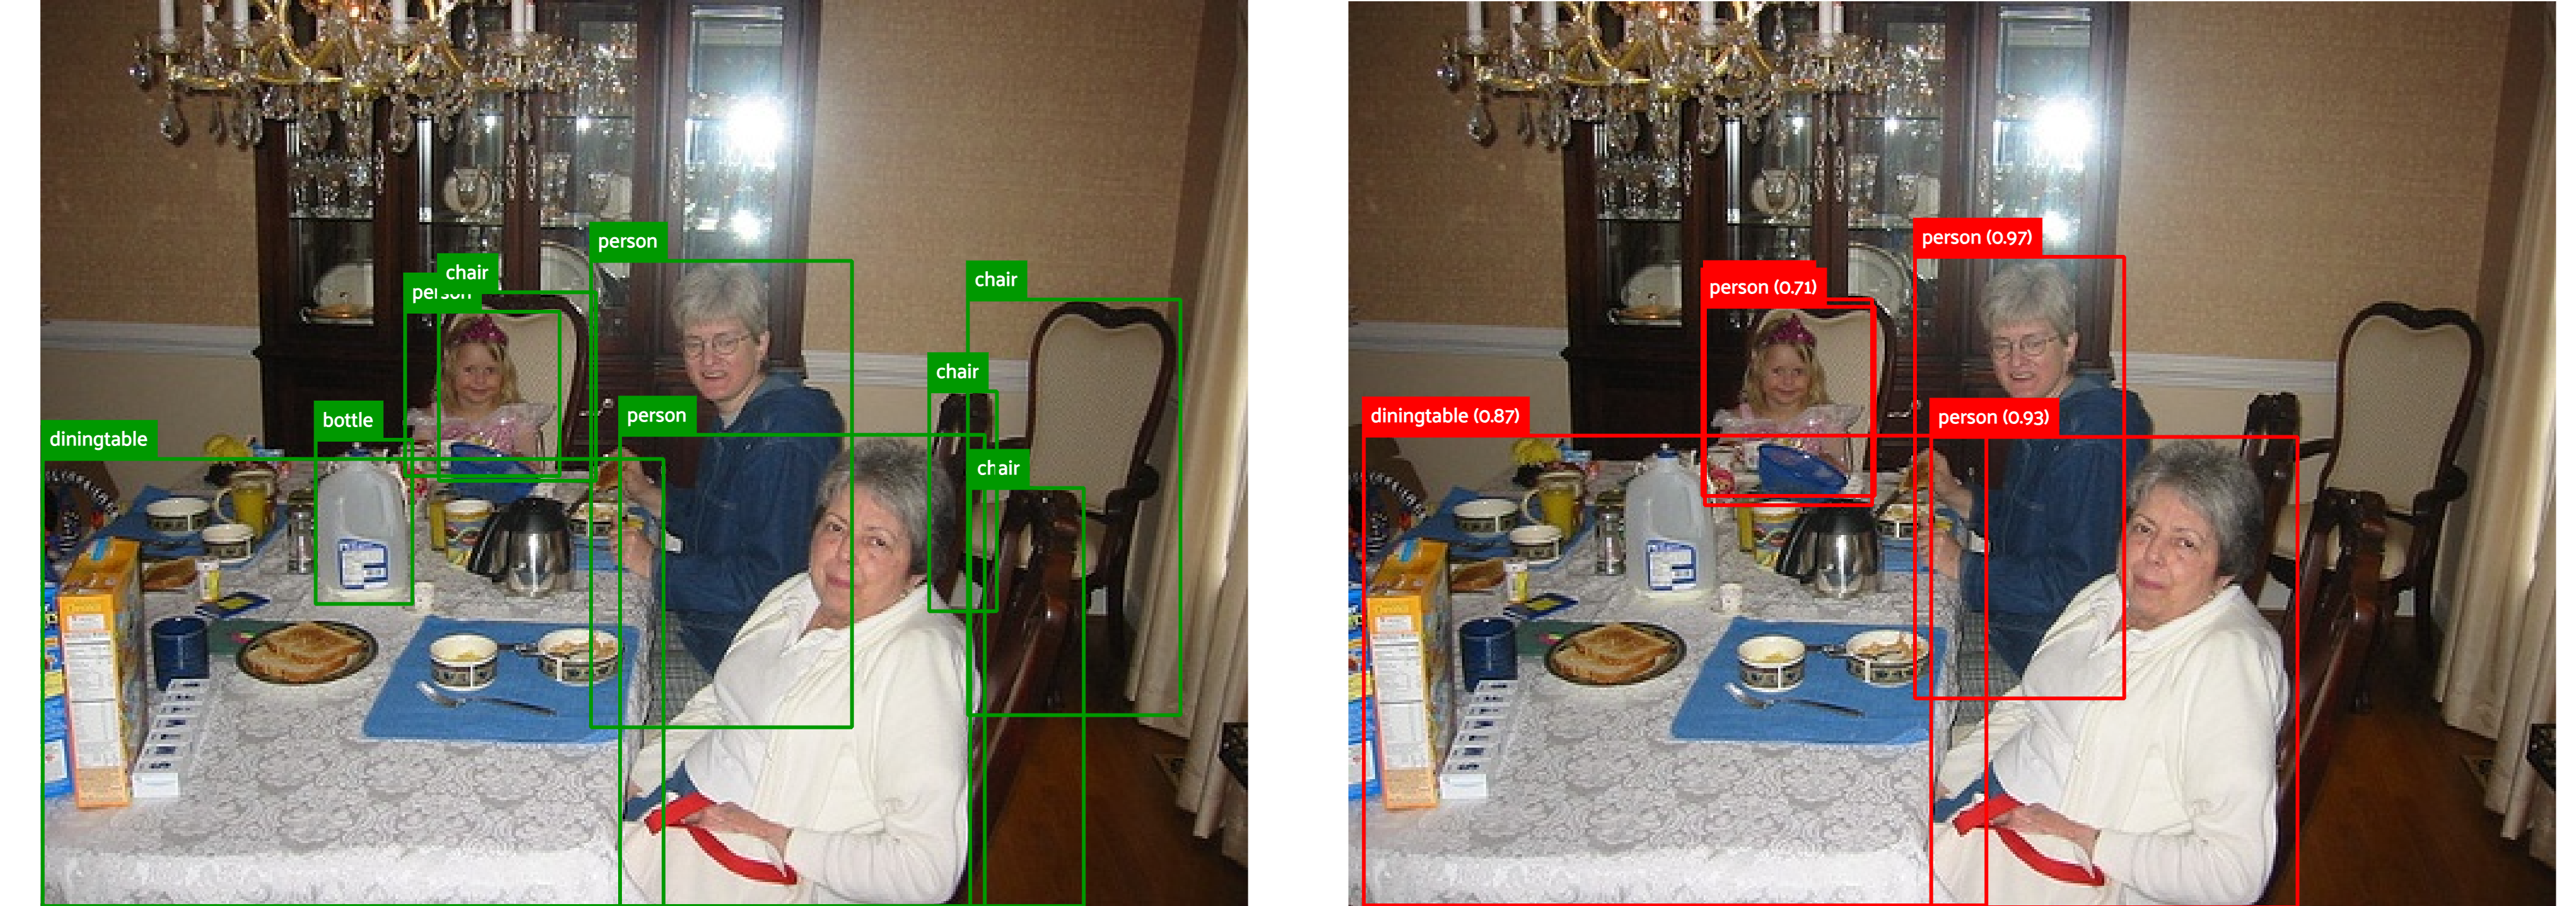
\includegraphics[width=0.5\textwidth]{images/ssd_res/ssd_b4.png}
    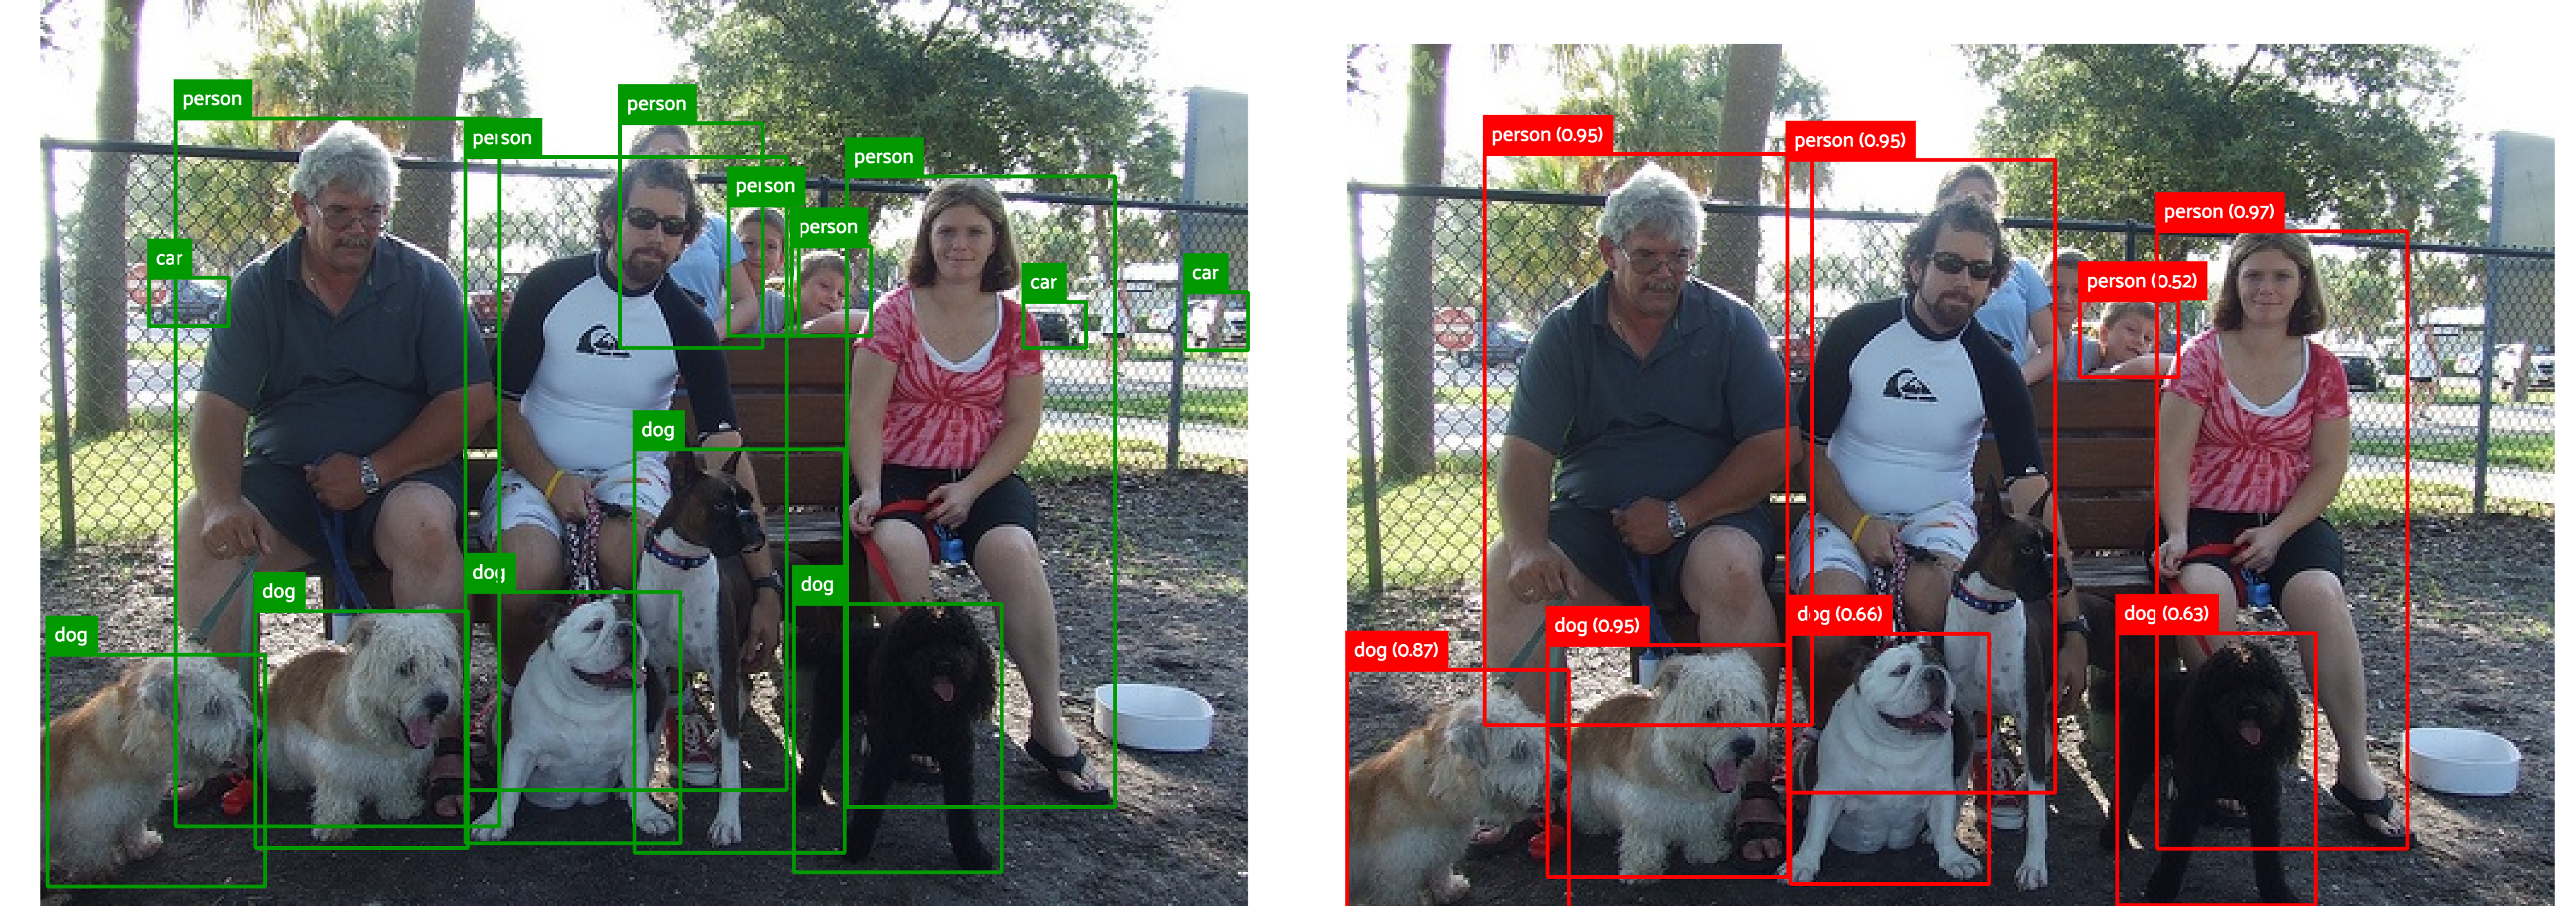
\includegraphics[width=0.5\textwidth]{images/ssd_res/ssd_b5.png}
    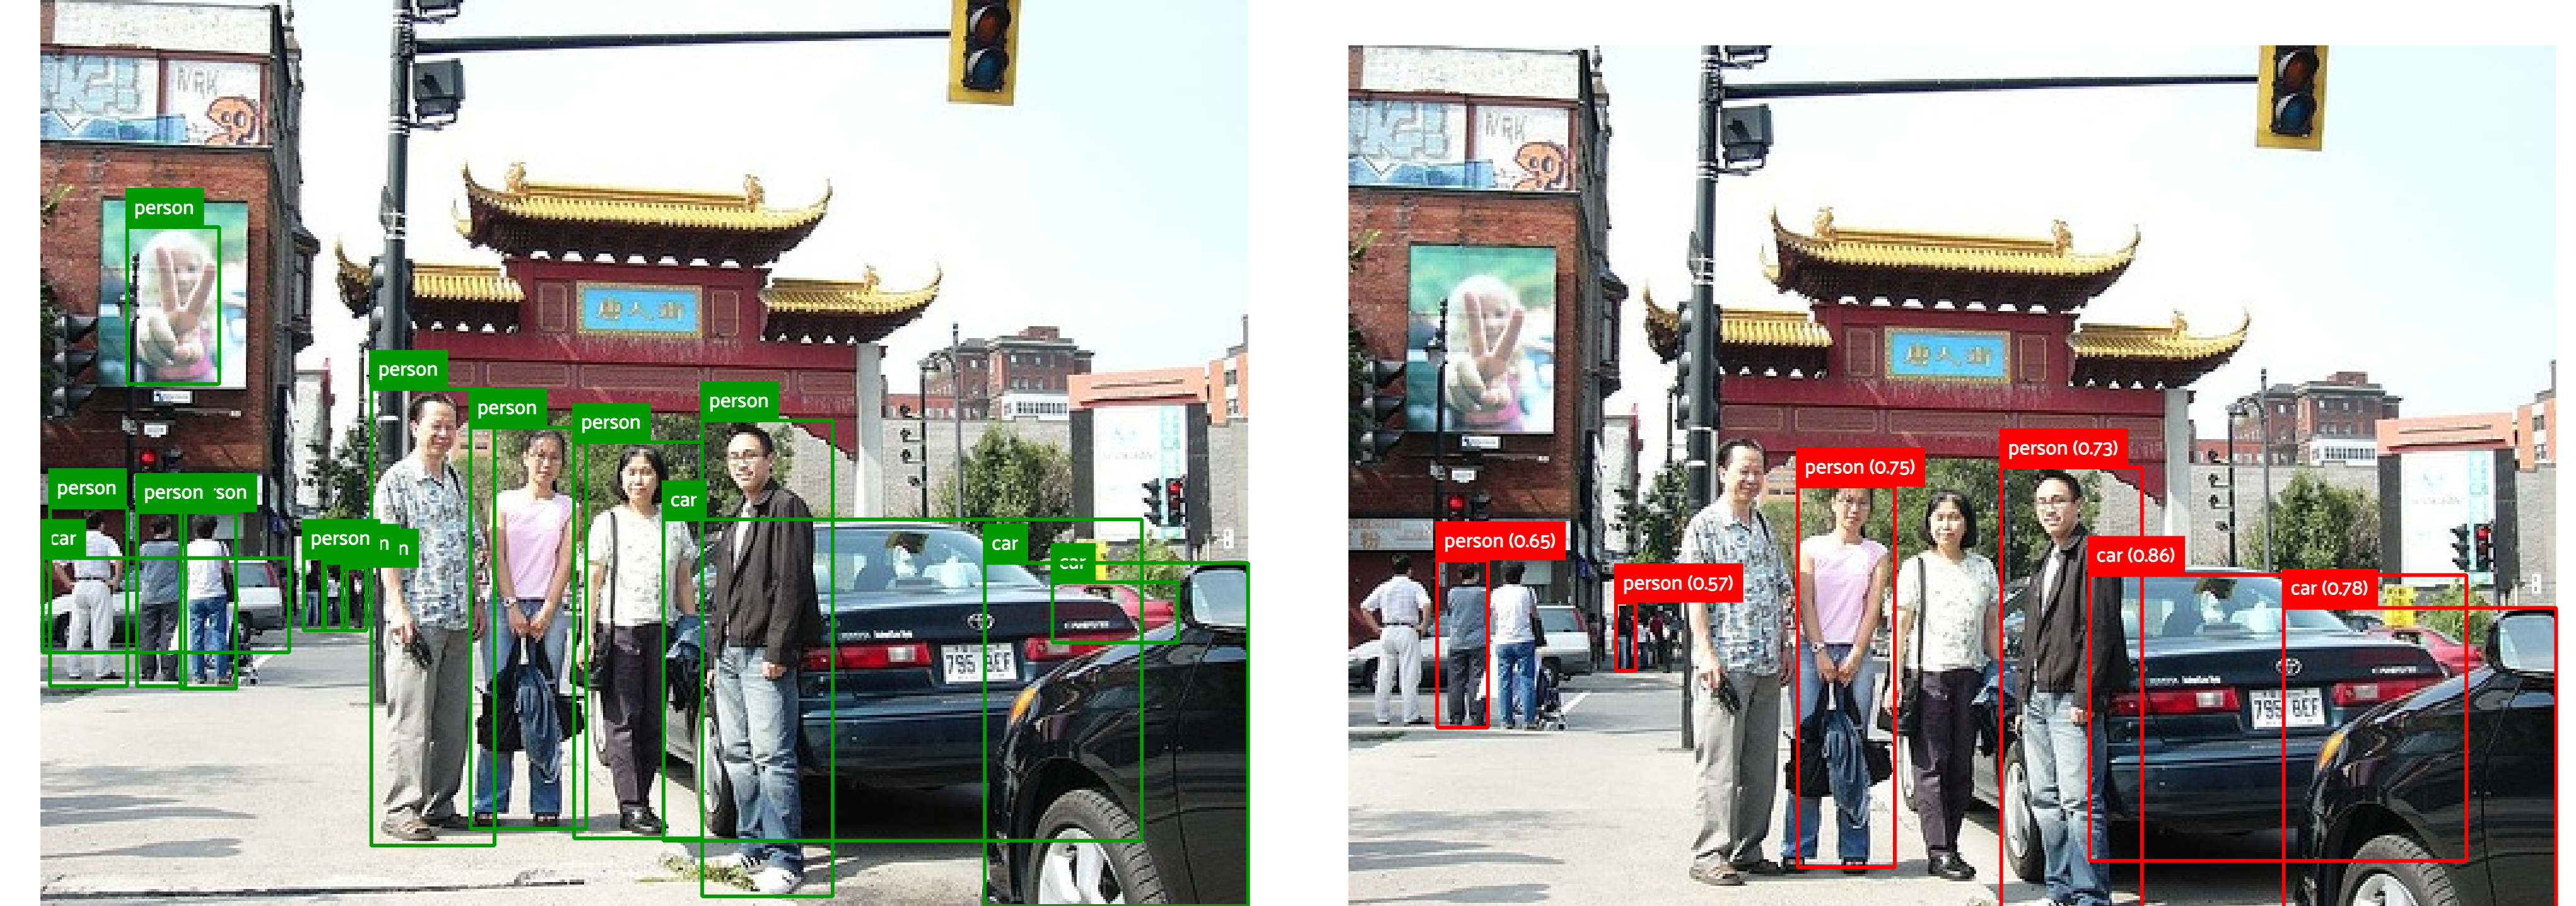
\includegraphics[width=0.5\textwidth]{images/ssd_res/ssd_b6.png}}
    \caption{SSD Best Predictions}
    \label{fig:ssd5}
\end{figure}

\begin{figure}[htbp]
    {\raggedright
    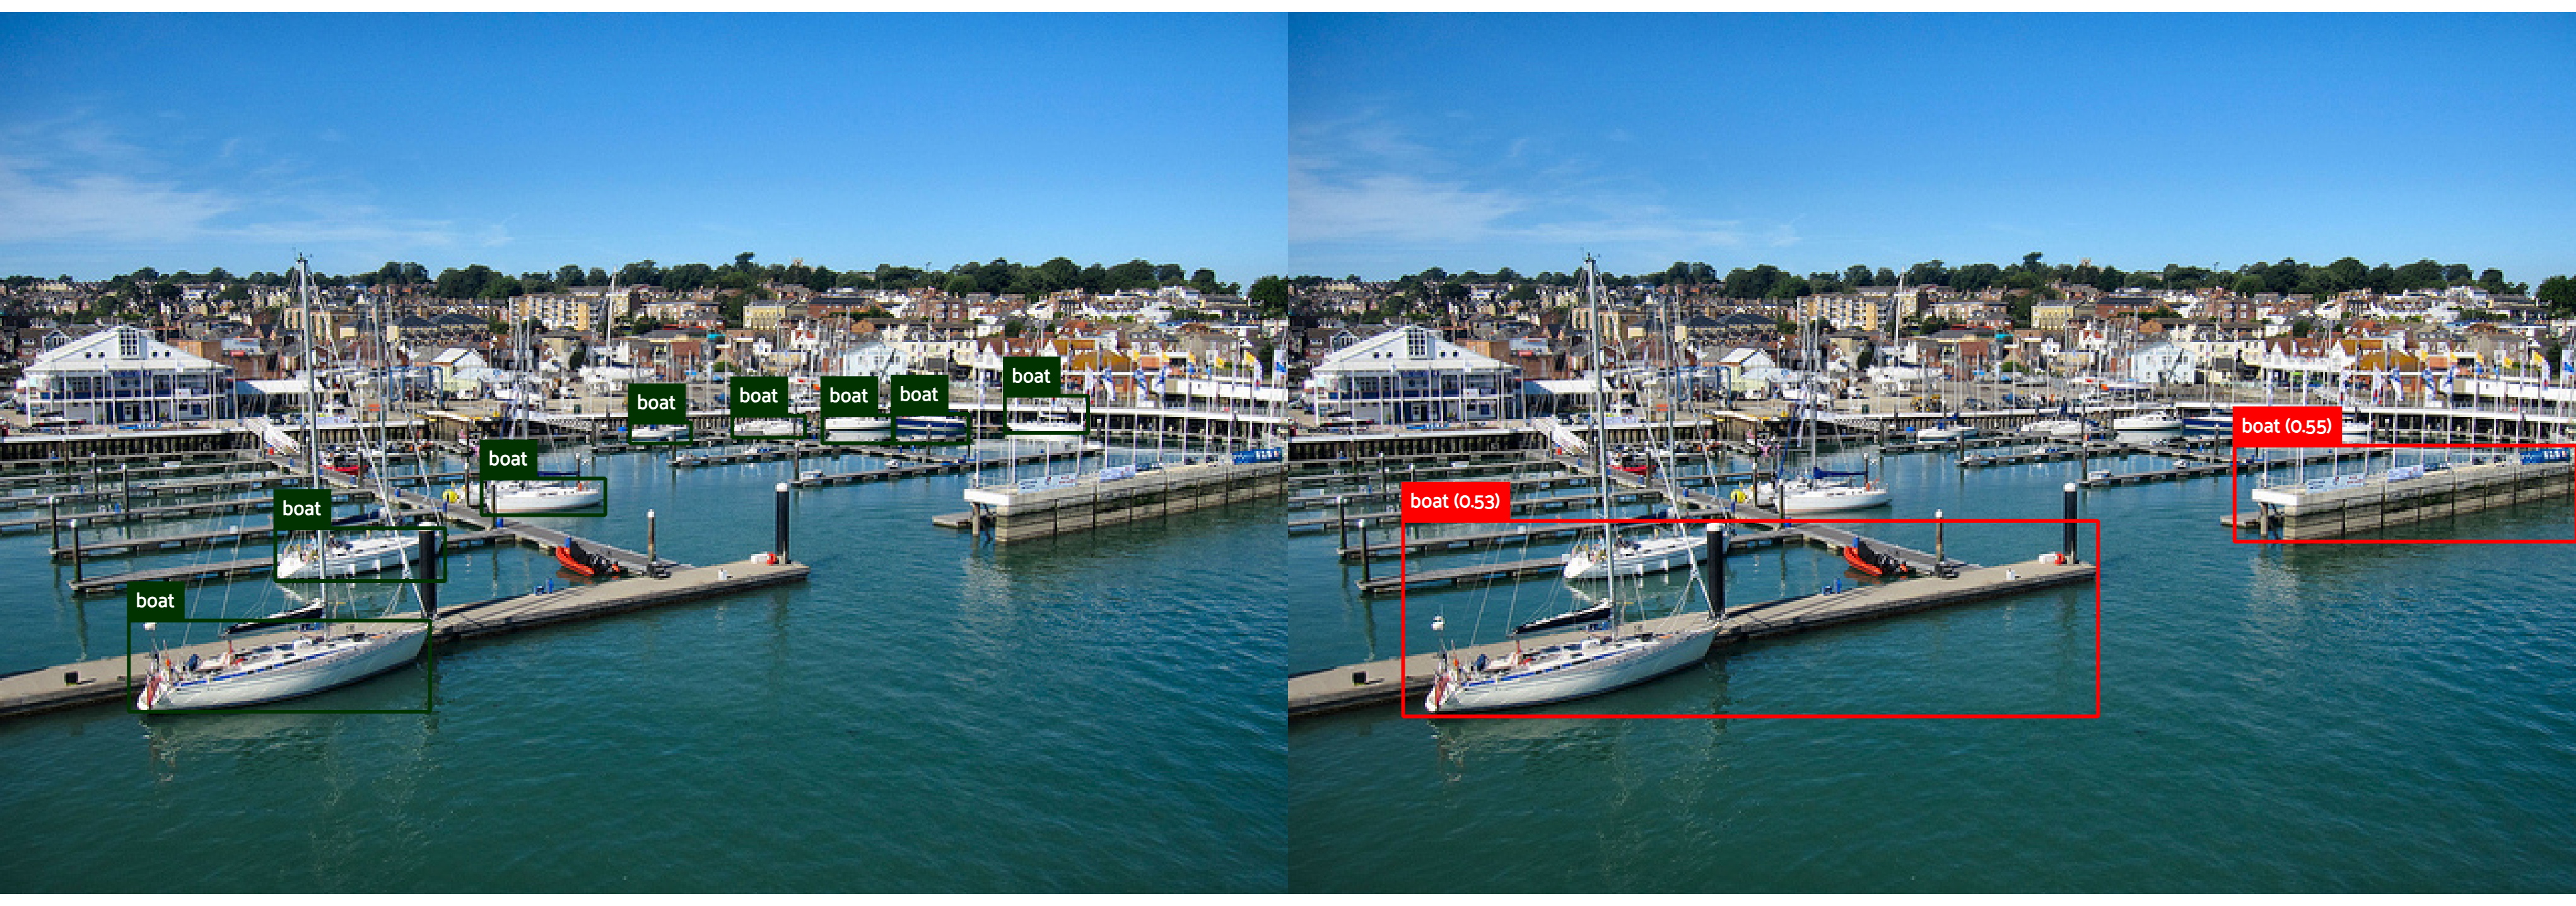
\includegraphics[width=0.5\textwidth]{images/ssd_res/ssd_w1.png}
    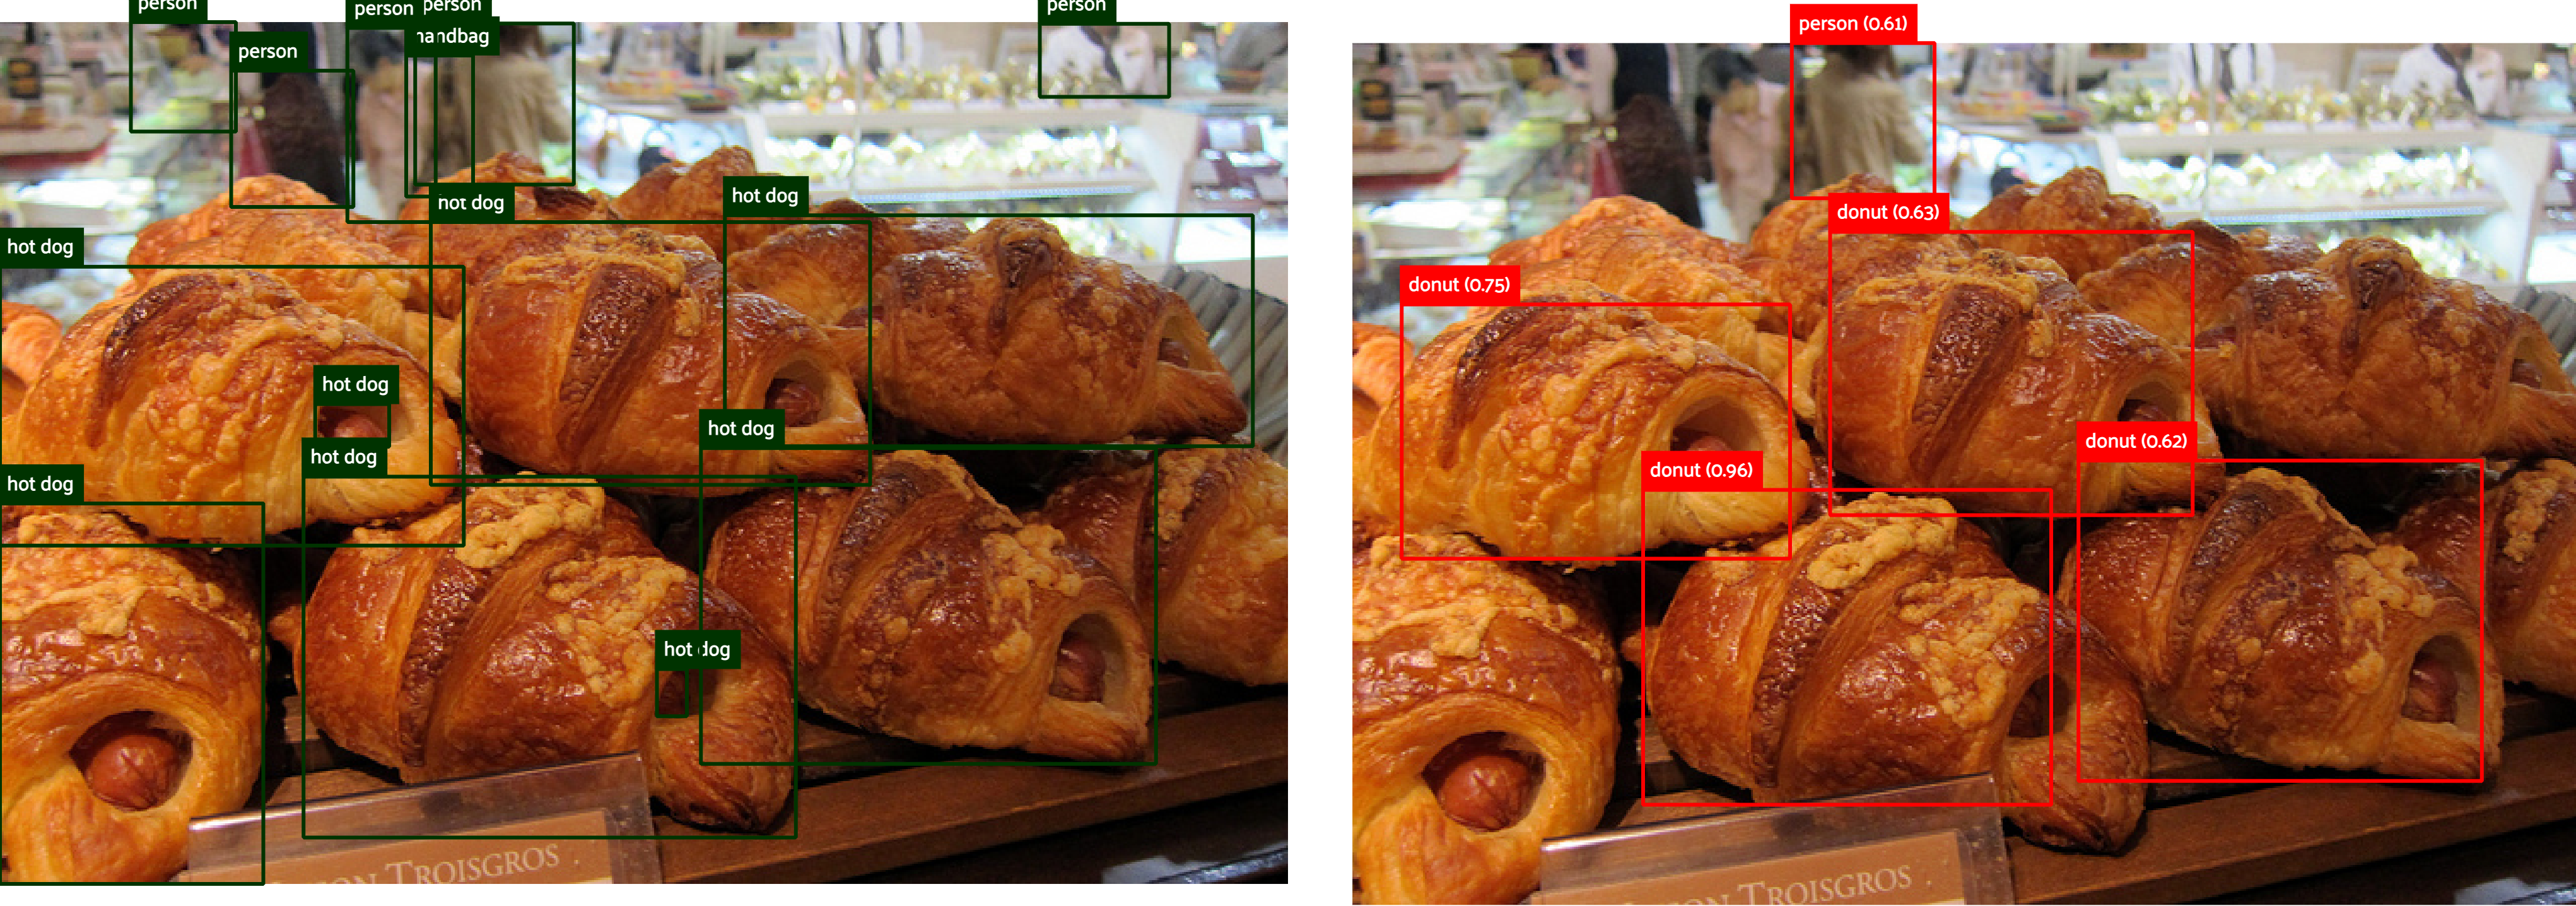
\includegraphics[width=0.5\textwidth]{images/ssd_res/ssd_w2.png}
    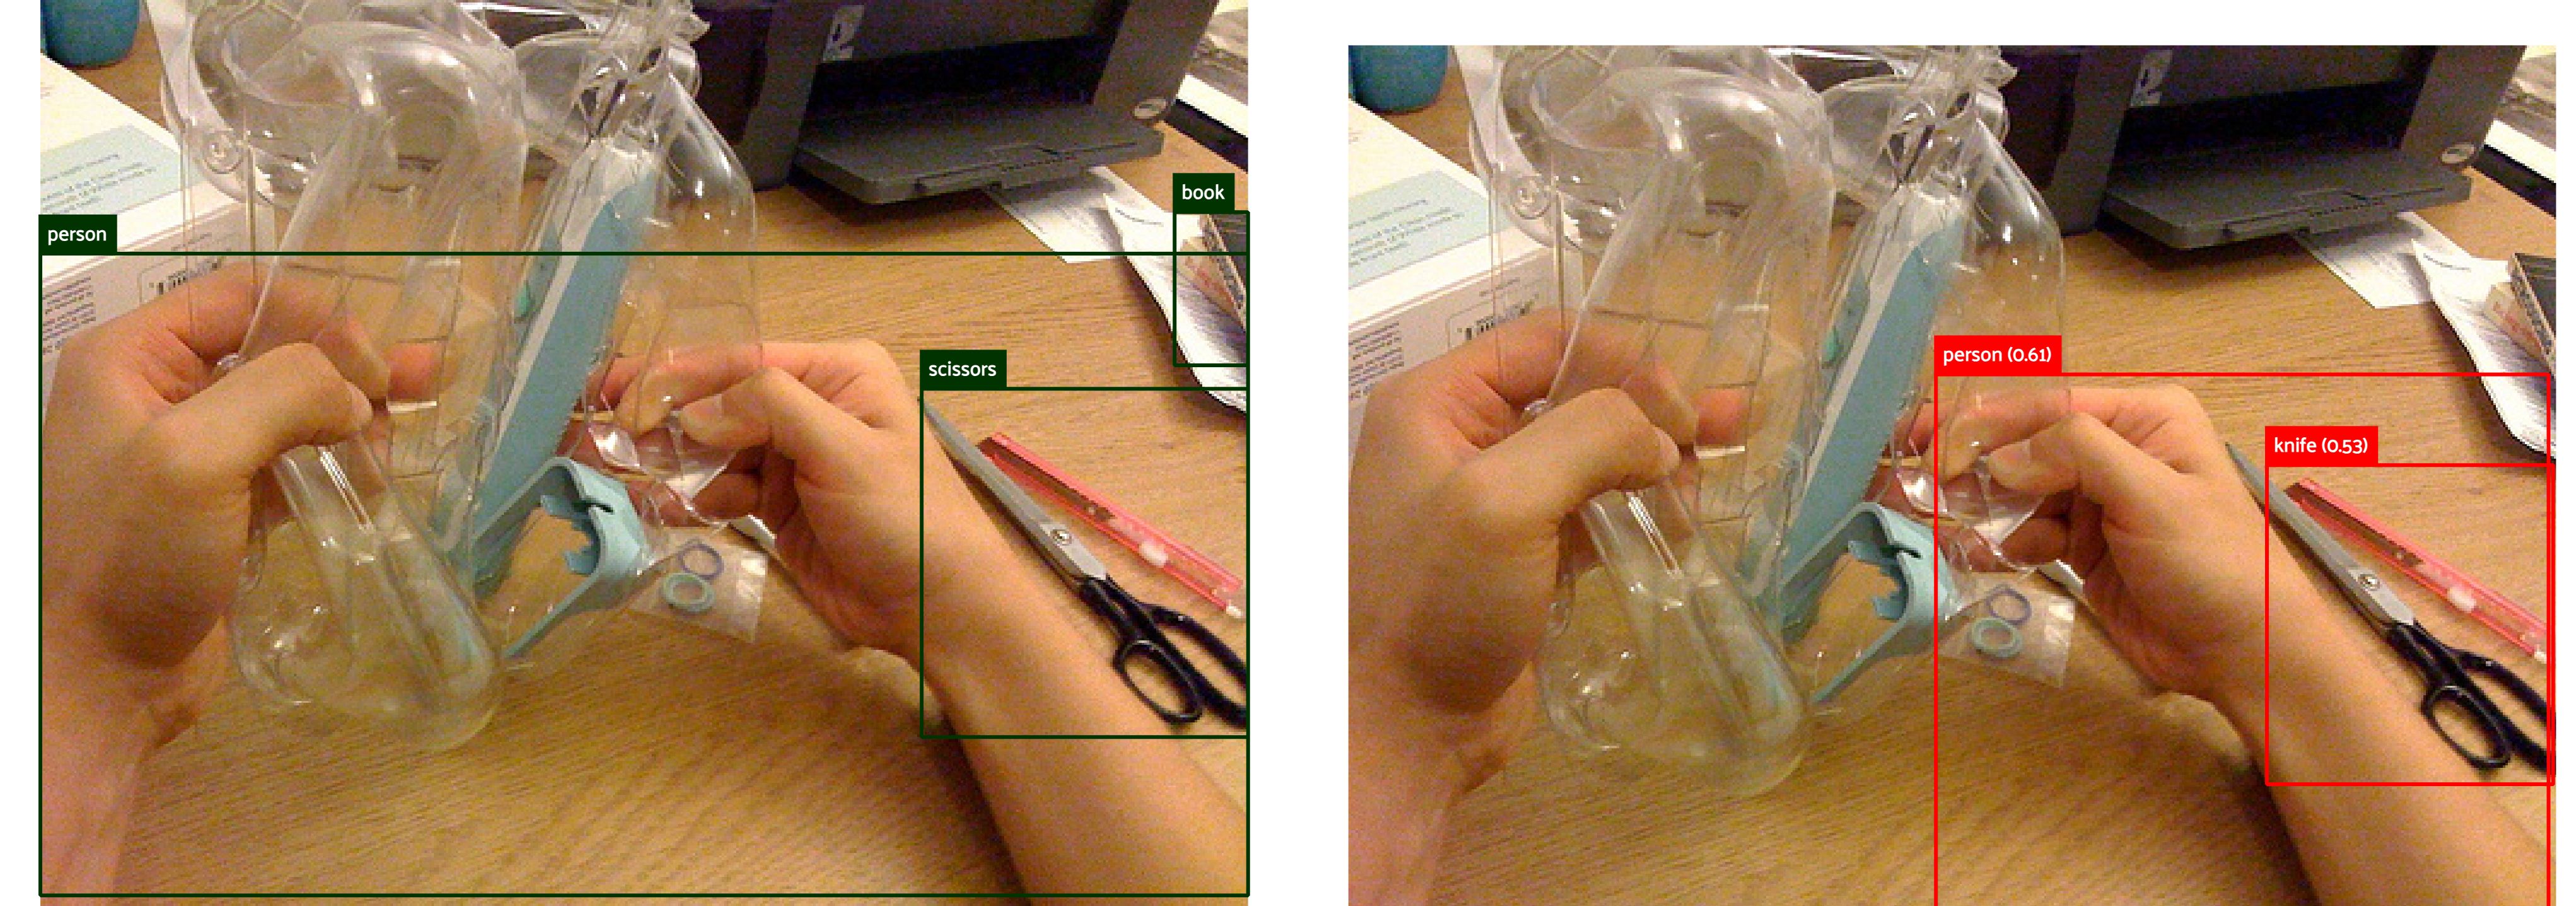
\includegraphics[width=0.5\textwidth]{images/ssd_res/ssd_w3.png}}
    {\raggedleft
    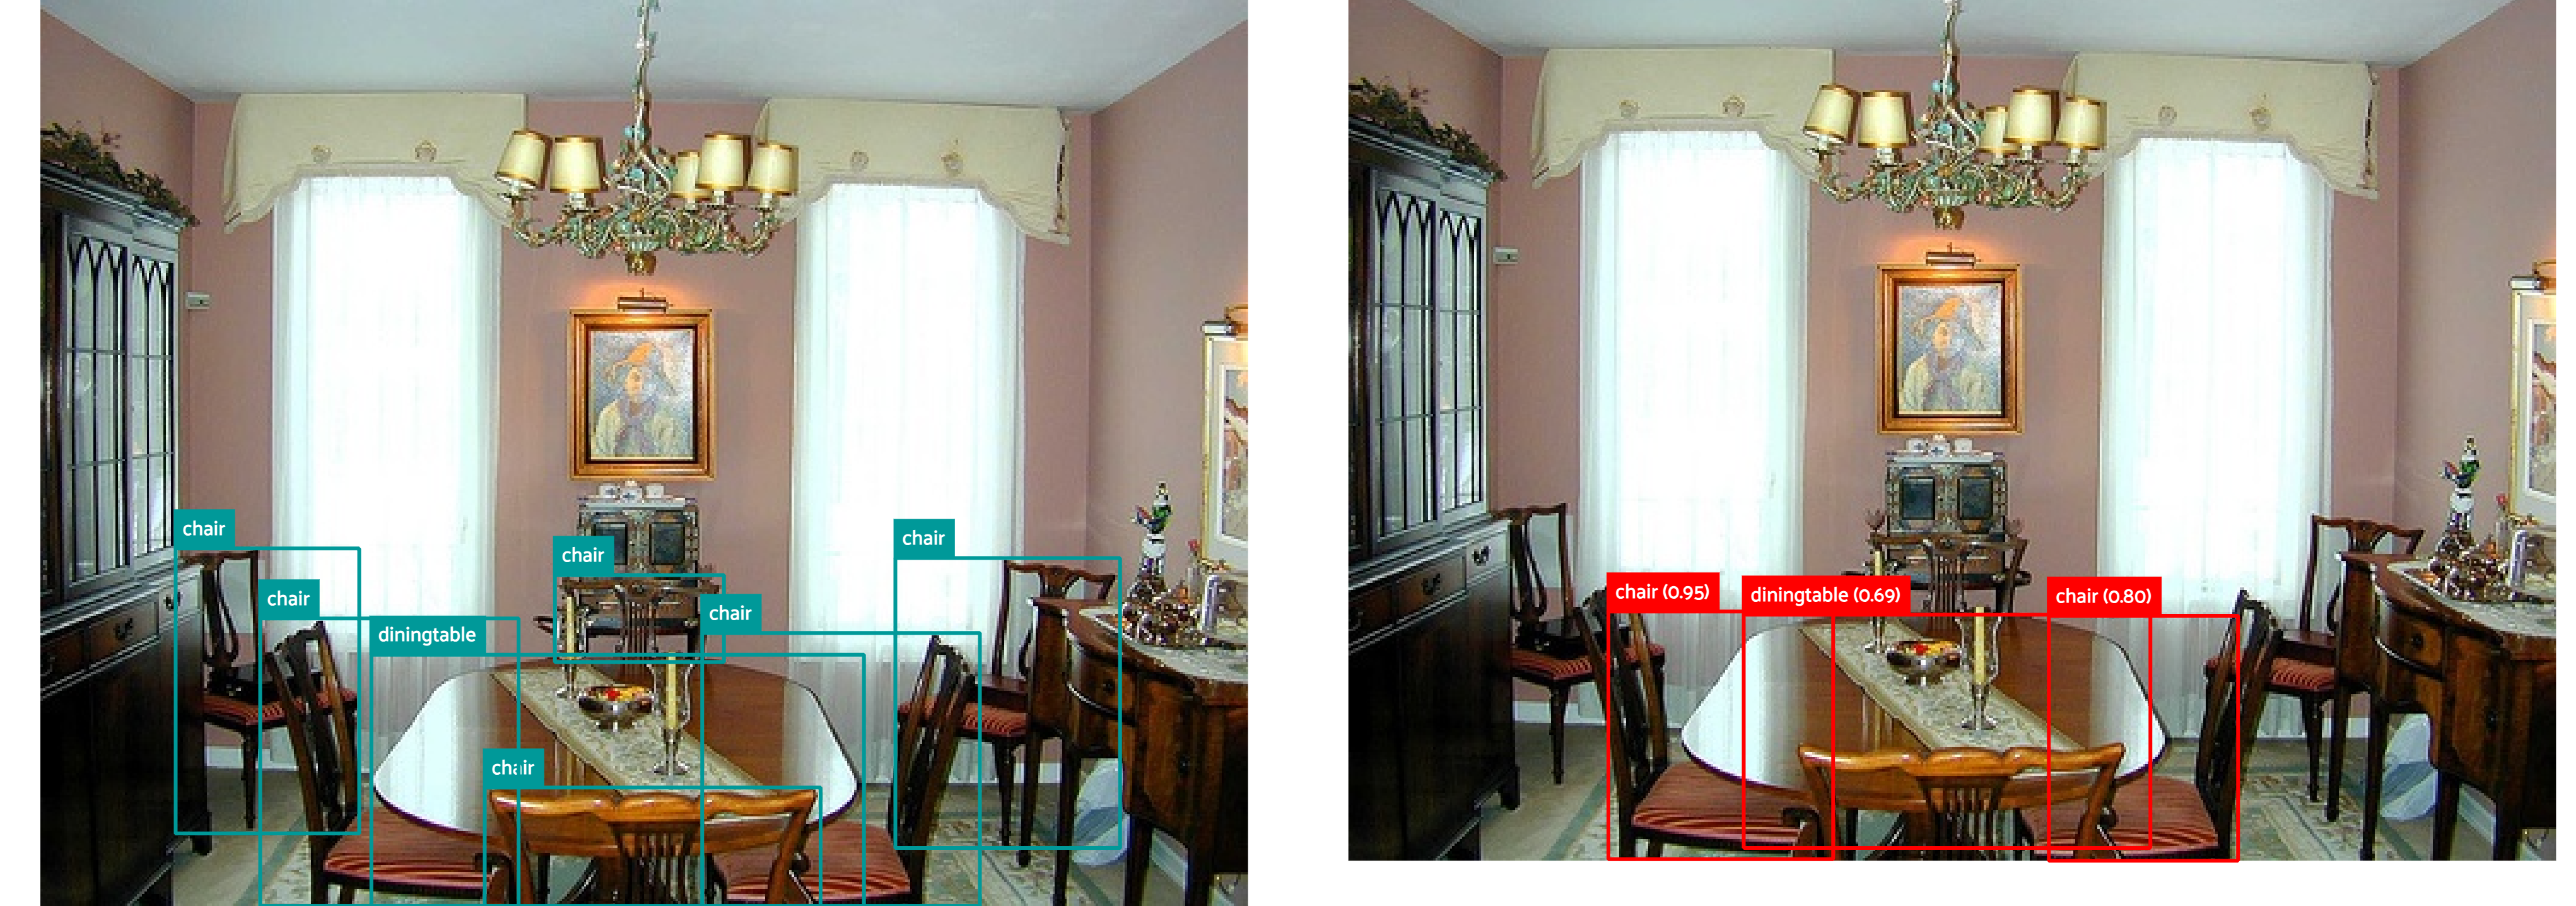
\includegraphics[width=0.5\textwidth]{images/ssd_res/ssd_w4.png}
    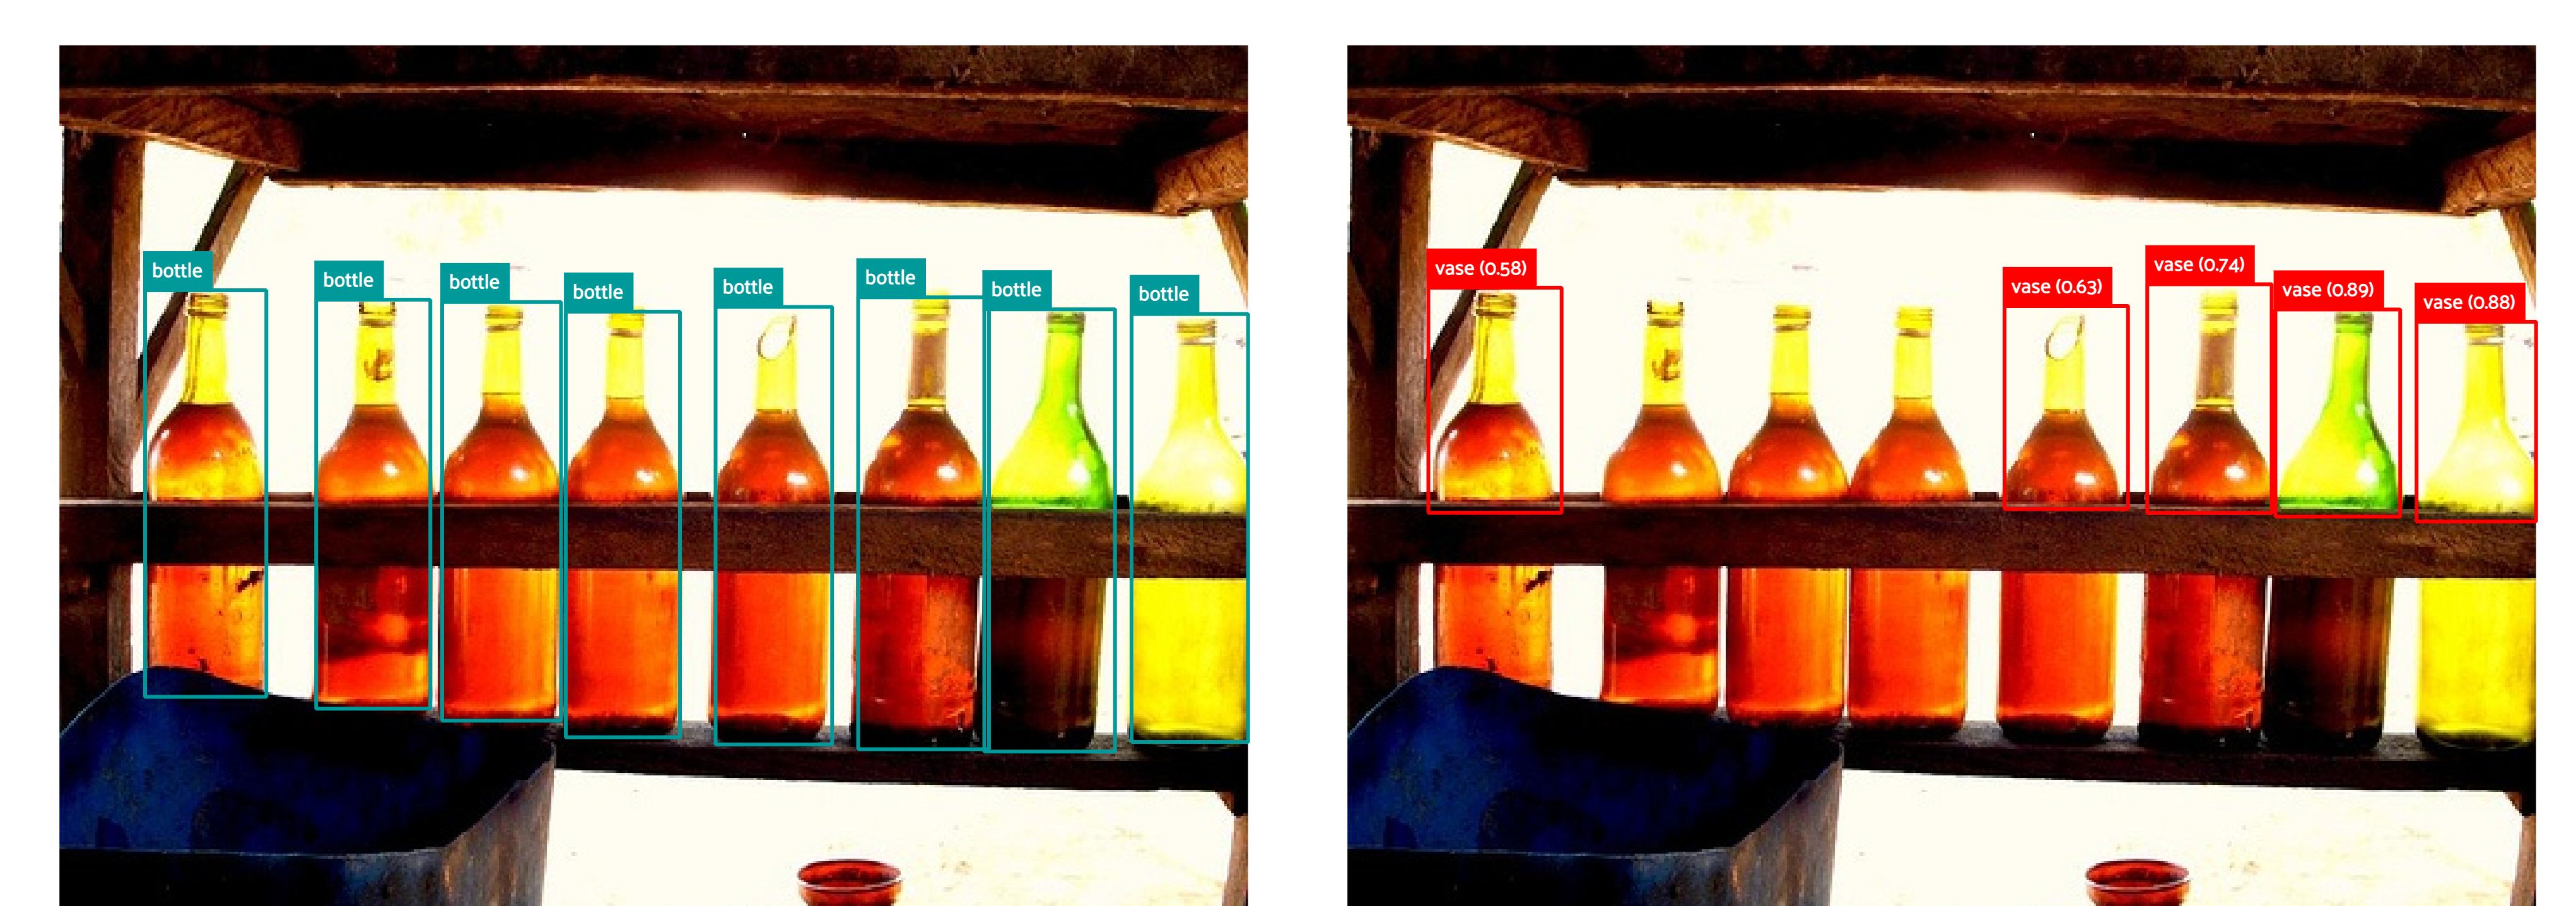
\includegraphics[width=0.5\textwidth]{images/ssd_res/ssd_w5.png}
    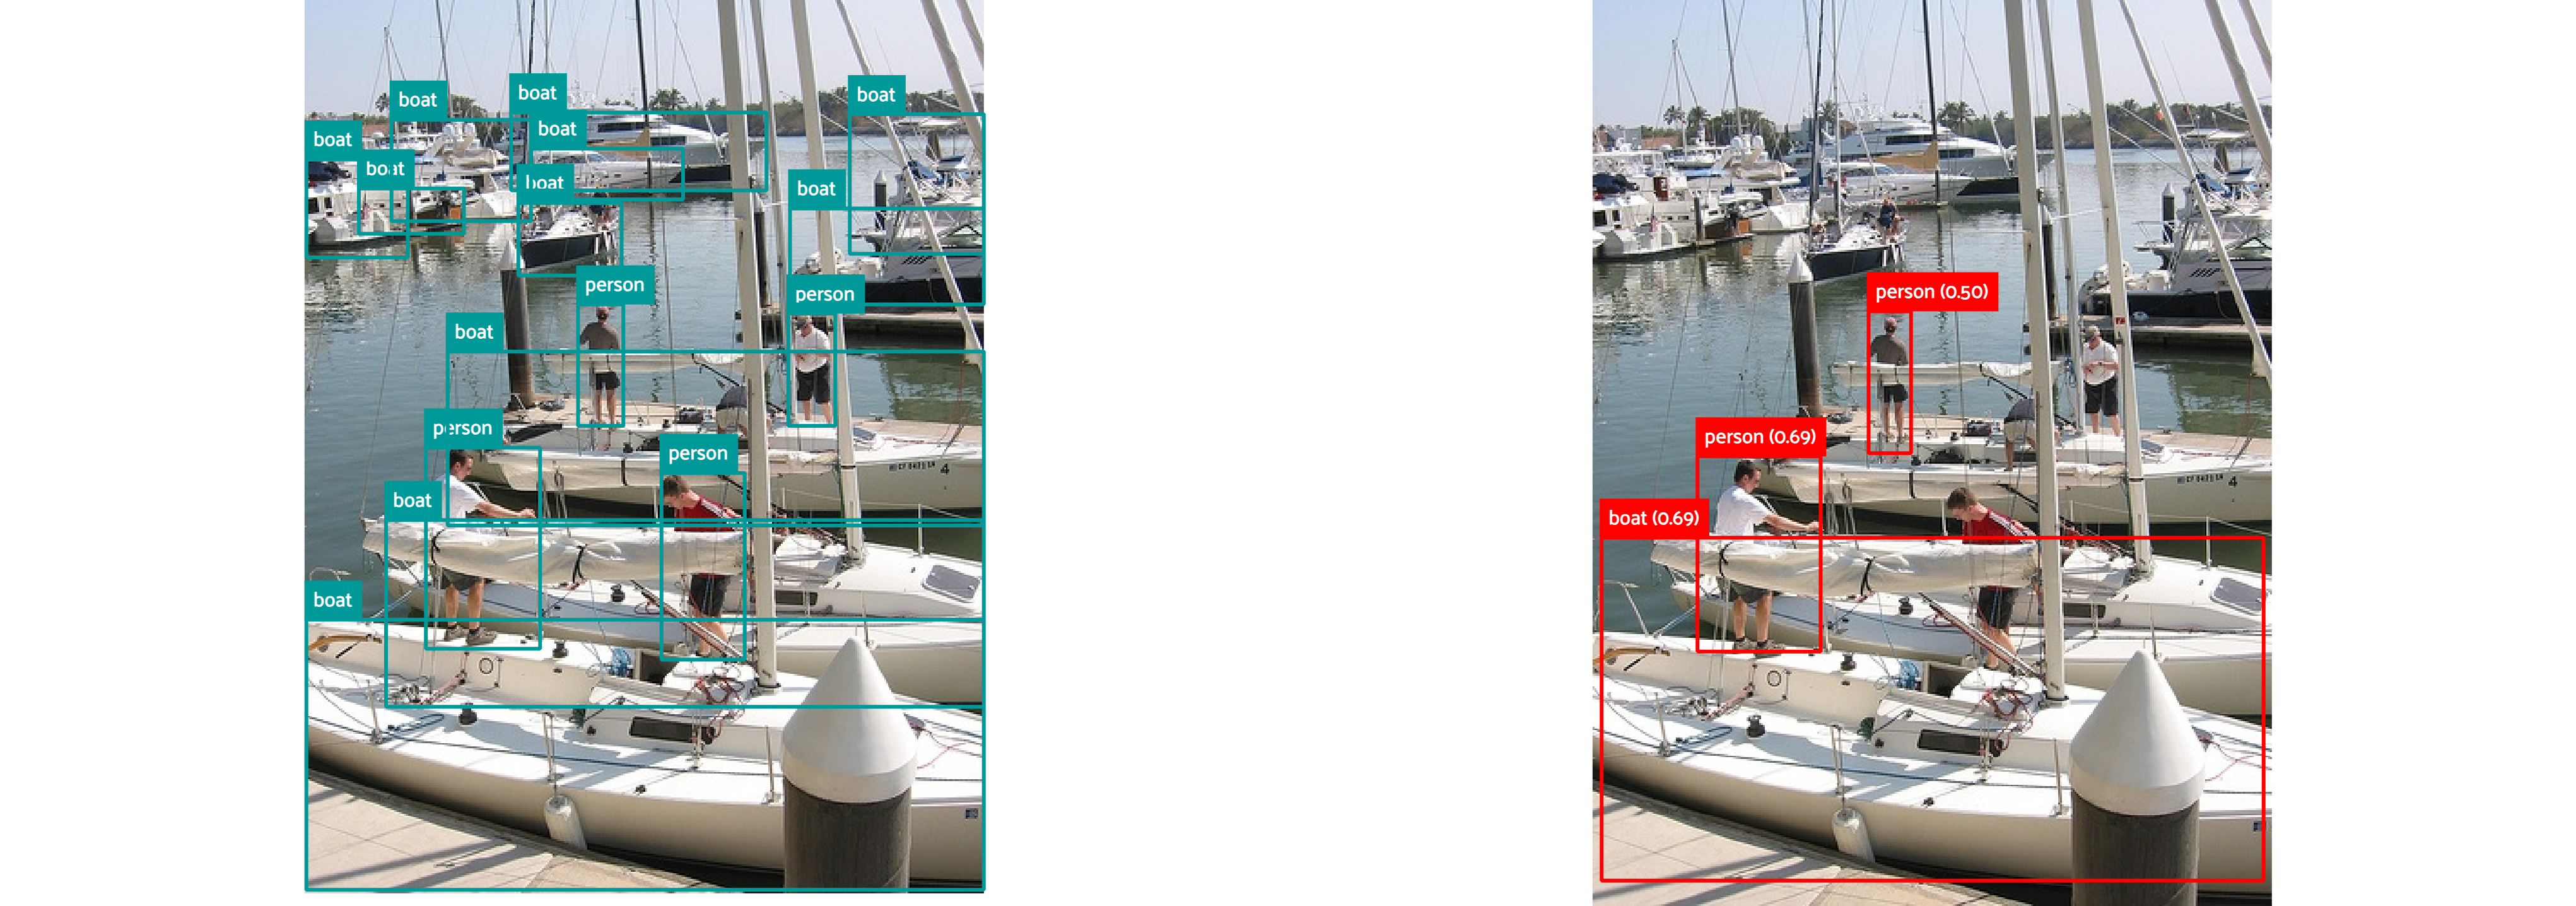
\includegraphics[width=0.5\textwidth]{images/ssd_res/ssd_w6.png}}
    \caption{SSD Worst Predictions}
    \label{fig:ssd6}
\end{figure}

Best predictions is at Figure \ref{fig:ssd5}.
\\
Worst predictions is at Figure \ref{fig:ssd6}.

\section{Faster R-CNN}

\subsection{Introduction}
There is no doubt that Fast R-CNN brings major improvements to traditional CNN. However, a major problem with Fast R-CNN is that it uses selective search to find all of the candidate boxes, which is quite time consuming.
\\
So is there a more efficient way to find these candidate boxes?
\\
Solution: Add in a neural network that extracts edges. In other words, use the neural network to find the candidate boxes.
\\
The neural network that does this kind of task is called Region Proposal Network (RPN).
\subsection{Architecture}
\begin{figure}[h]
    \centering
    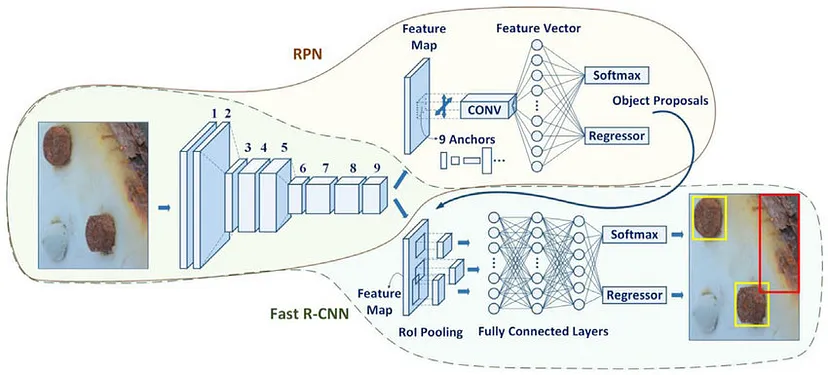
\includegraphics[width=0.75\textwidth]{images/rcnn_arch.png}
    \caption{Faster R-CNN Architecture}
    \label{fig:rcnn1}
\end{figure}
\paragraph{Part 1 : Convolution layers}
In this layers we train filters to extract the appropriate features the image, for example let’s say that we are going to train those filters to extract the appropriate features for a human face, then those filters are going to learn throught training shapes and colors that only exist in the human face.

\paragraph{Part 2 : Region Proposel Network (RPN)}

RPN is small neural network sliding on the last feature map of the convolution layers and predict whether there is an object or not and also predict the bounding box of those objects.

\paragraph{Part 3 : Classes and Bounding Boxes prediction}

Now we use another Fully connected neural networks that takes as an input the regions proposed by the RPN and predict object class (classification) and Bounding boxes (Regression).


\subsection{Inference Results}

\begin{figure}[htbp]
    {\raggedright
    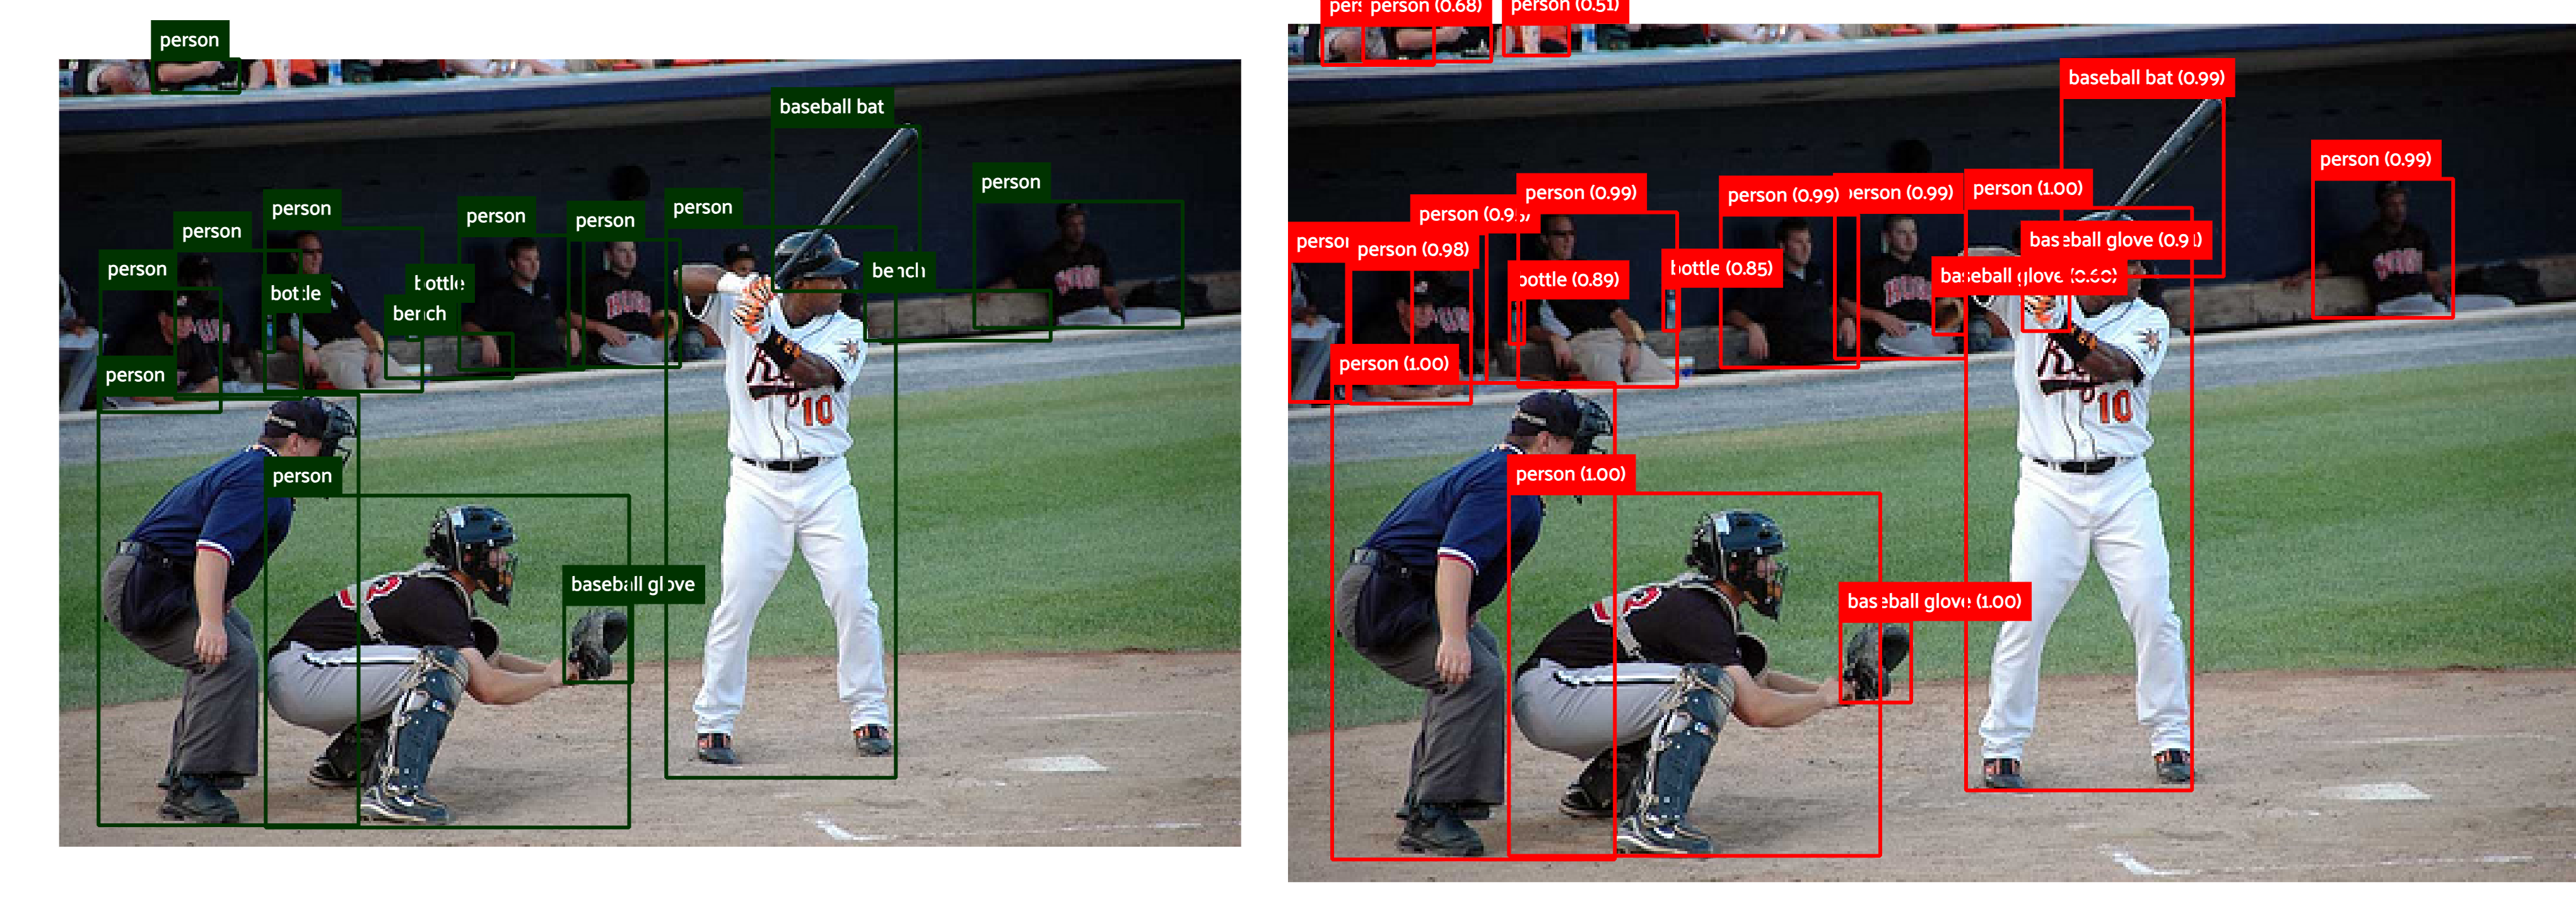
\includegraphics[width=0.5\textwidth]{images/rcnn_res/rcnn_b1.png}
    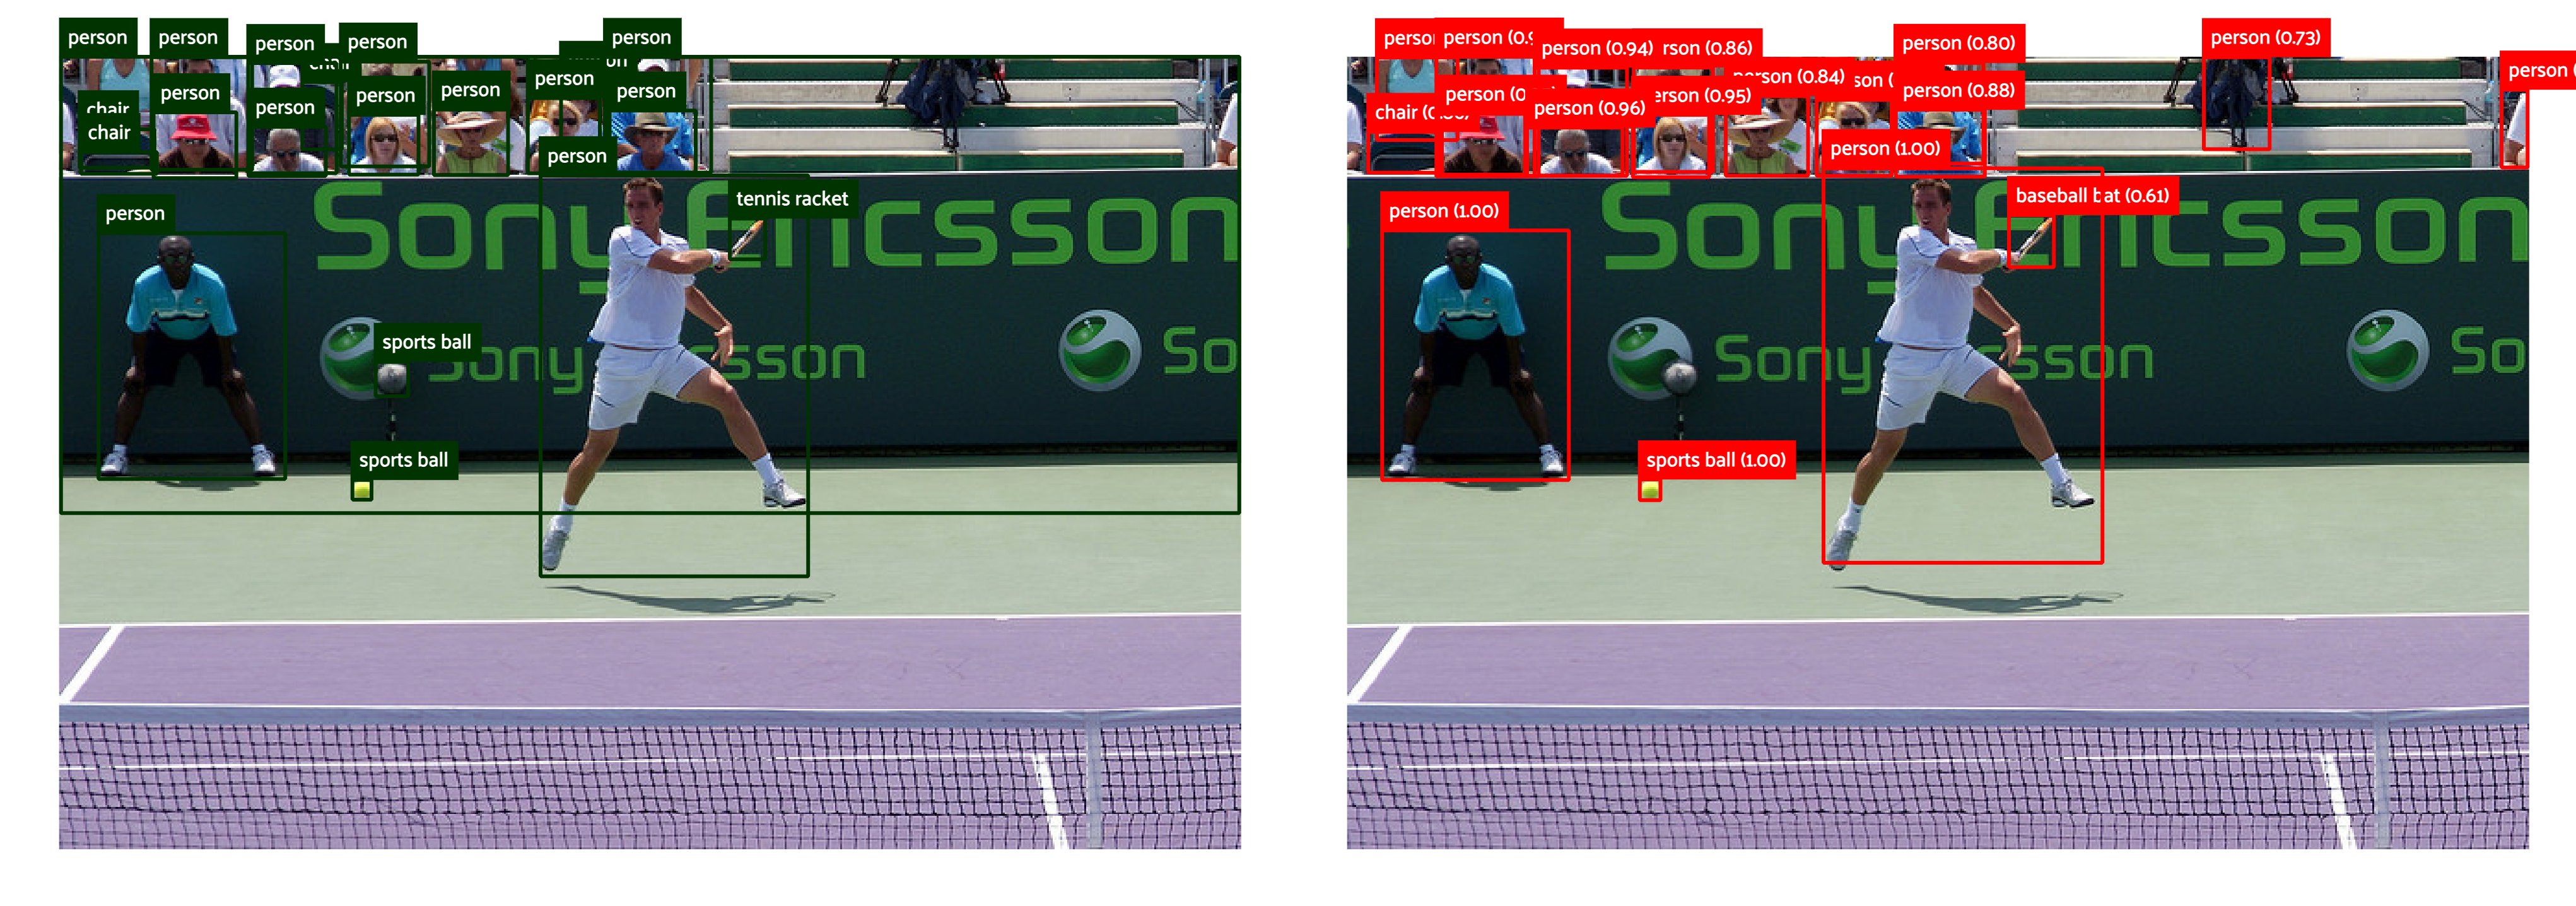
\includegraphics[width=0.5\textwidth]{images/rcnn_res/rcnn_b2.png}
    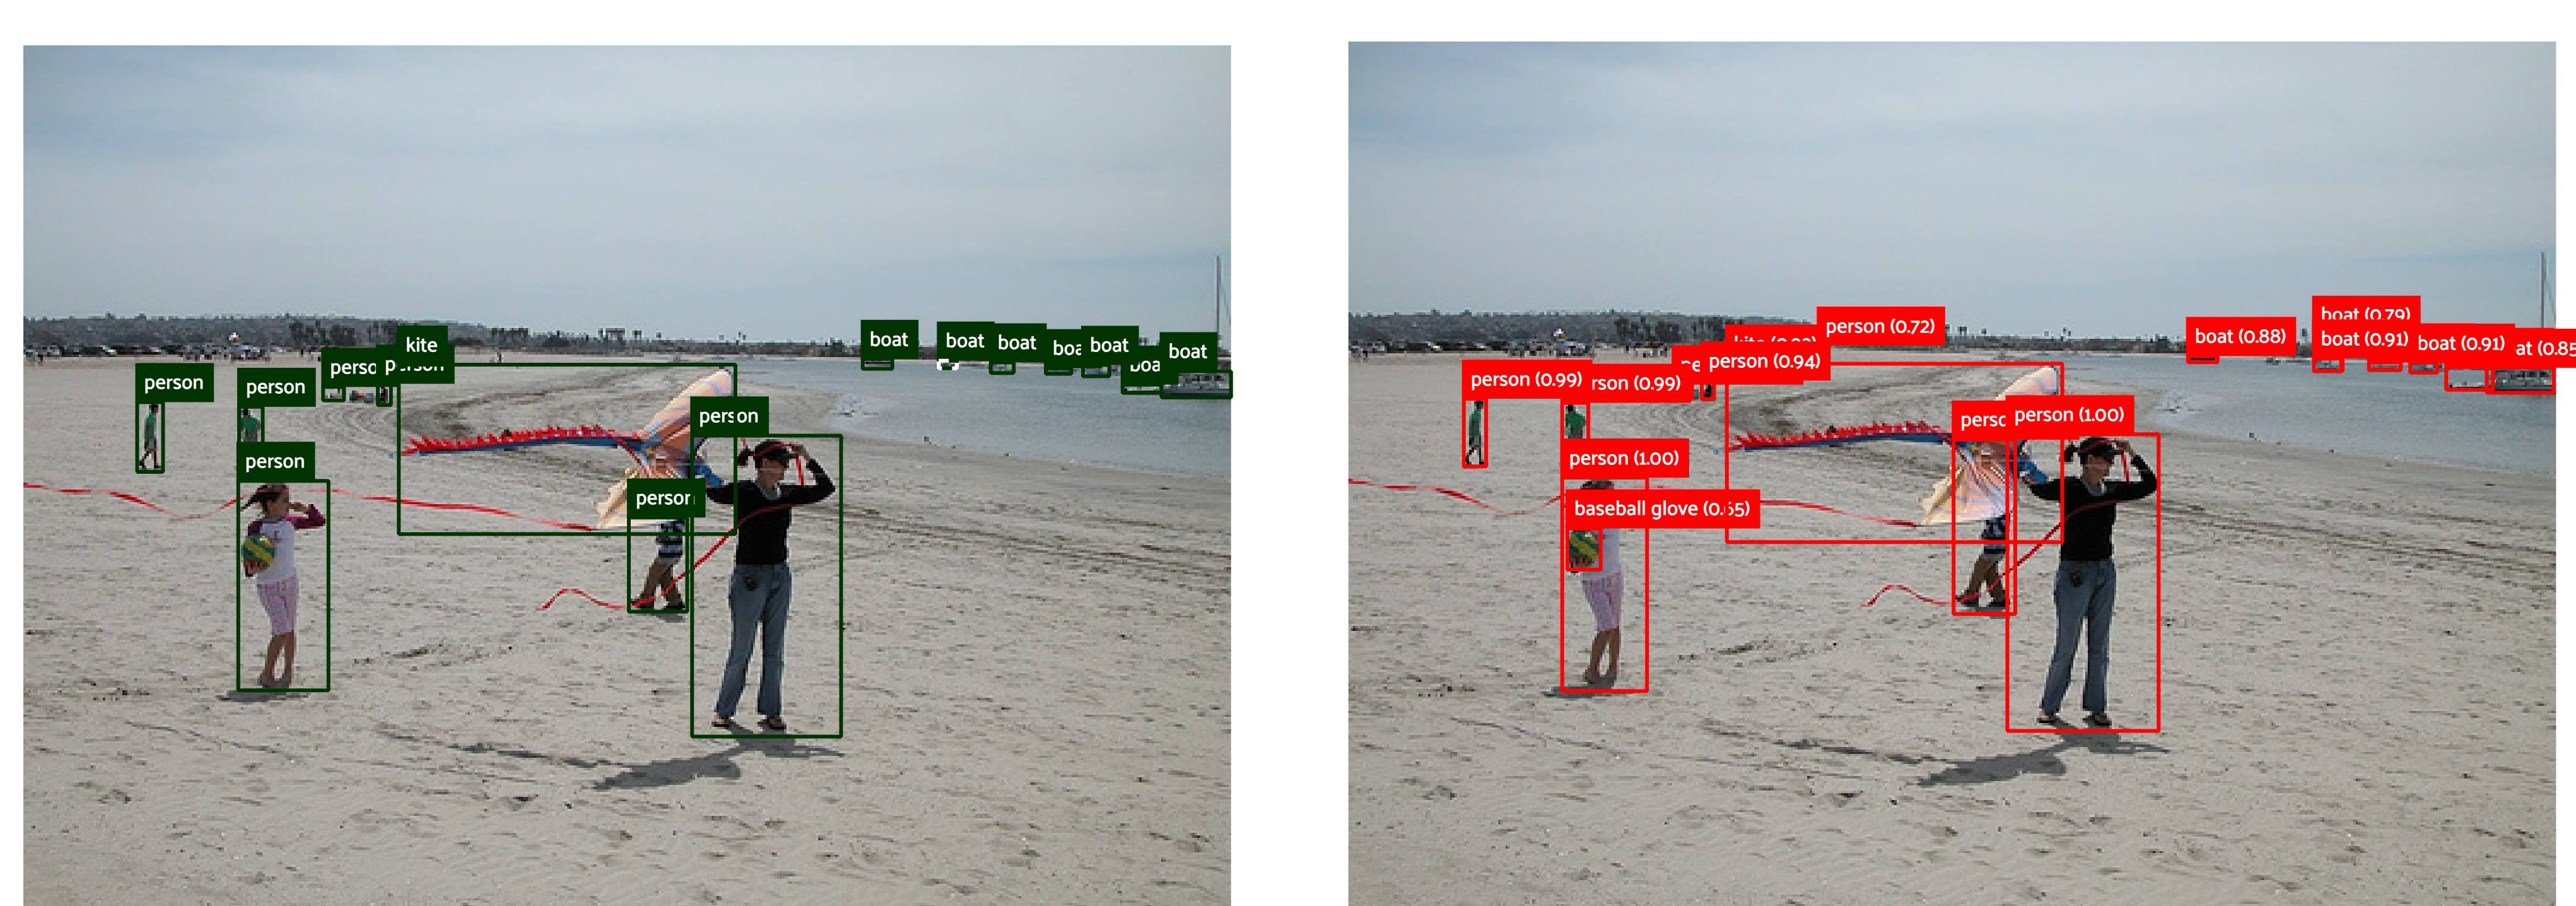
\includegraphics[width=0.5\textwidth]{images/rcnn_res/rcnn_b3.png}}
    {\raggedleft
    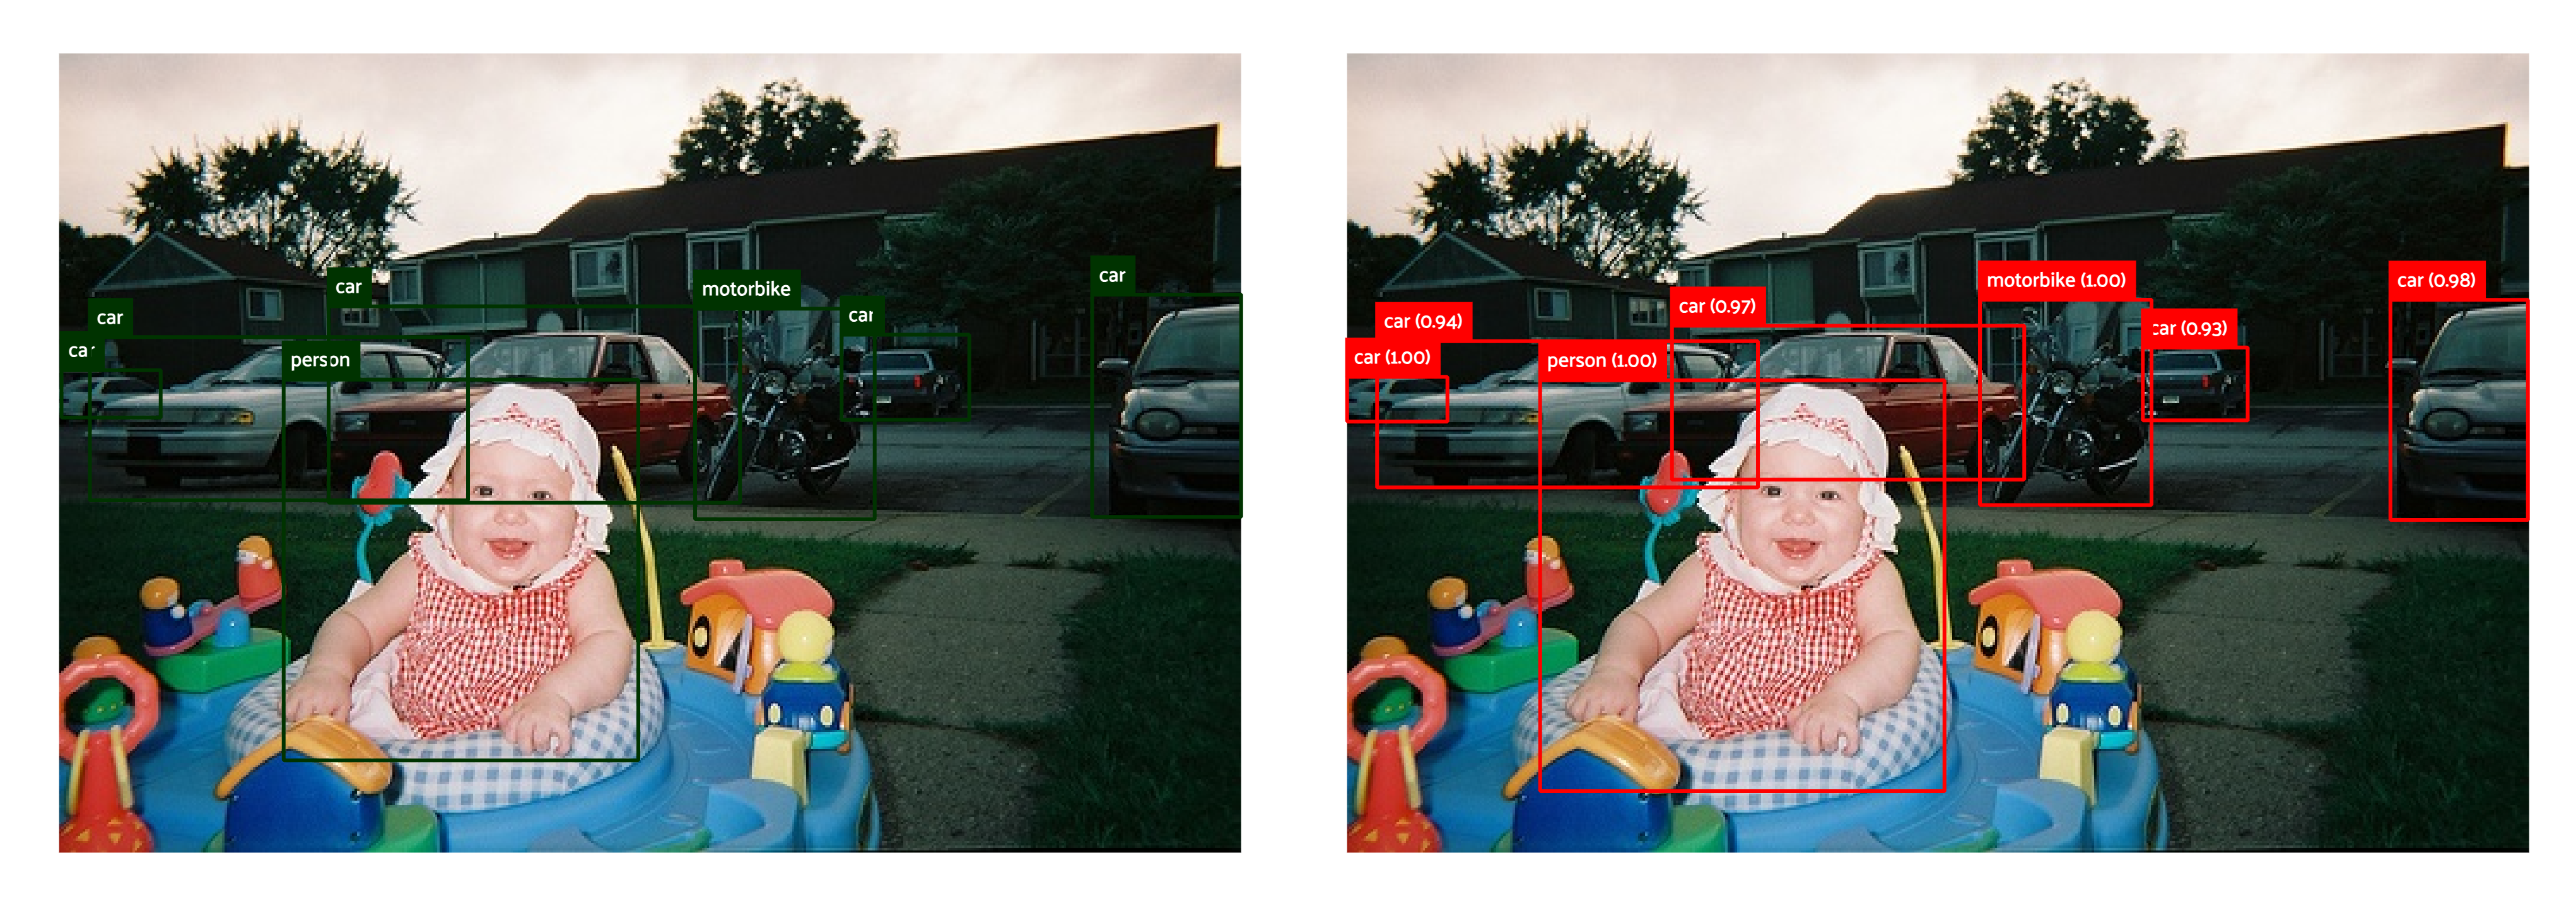
\includegraphics[width=0.5\textwidth]{images/rcnn_res/rcnn_b4.png}
    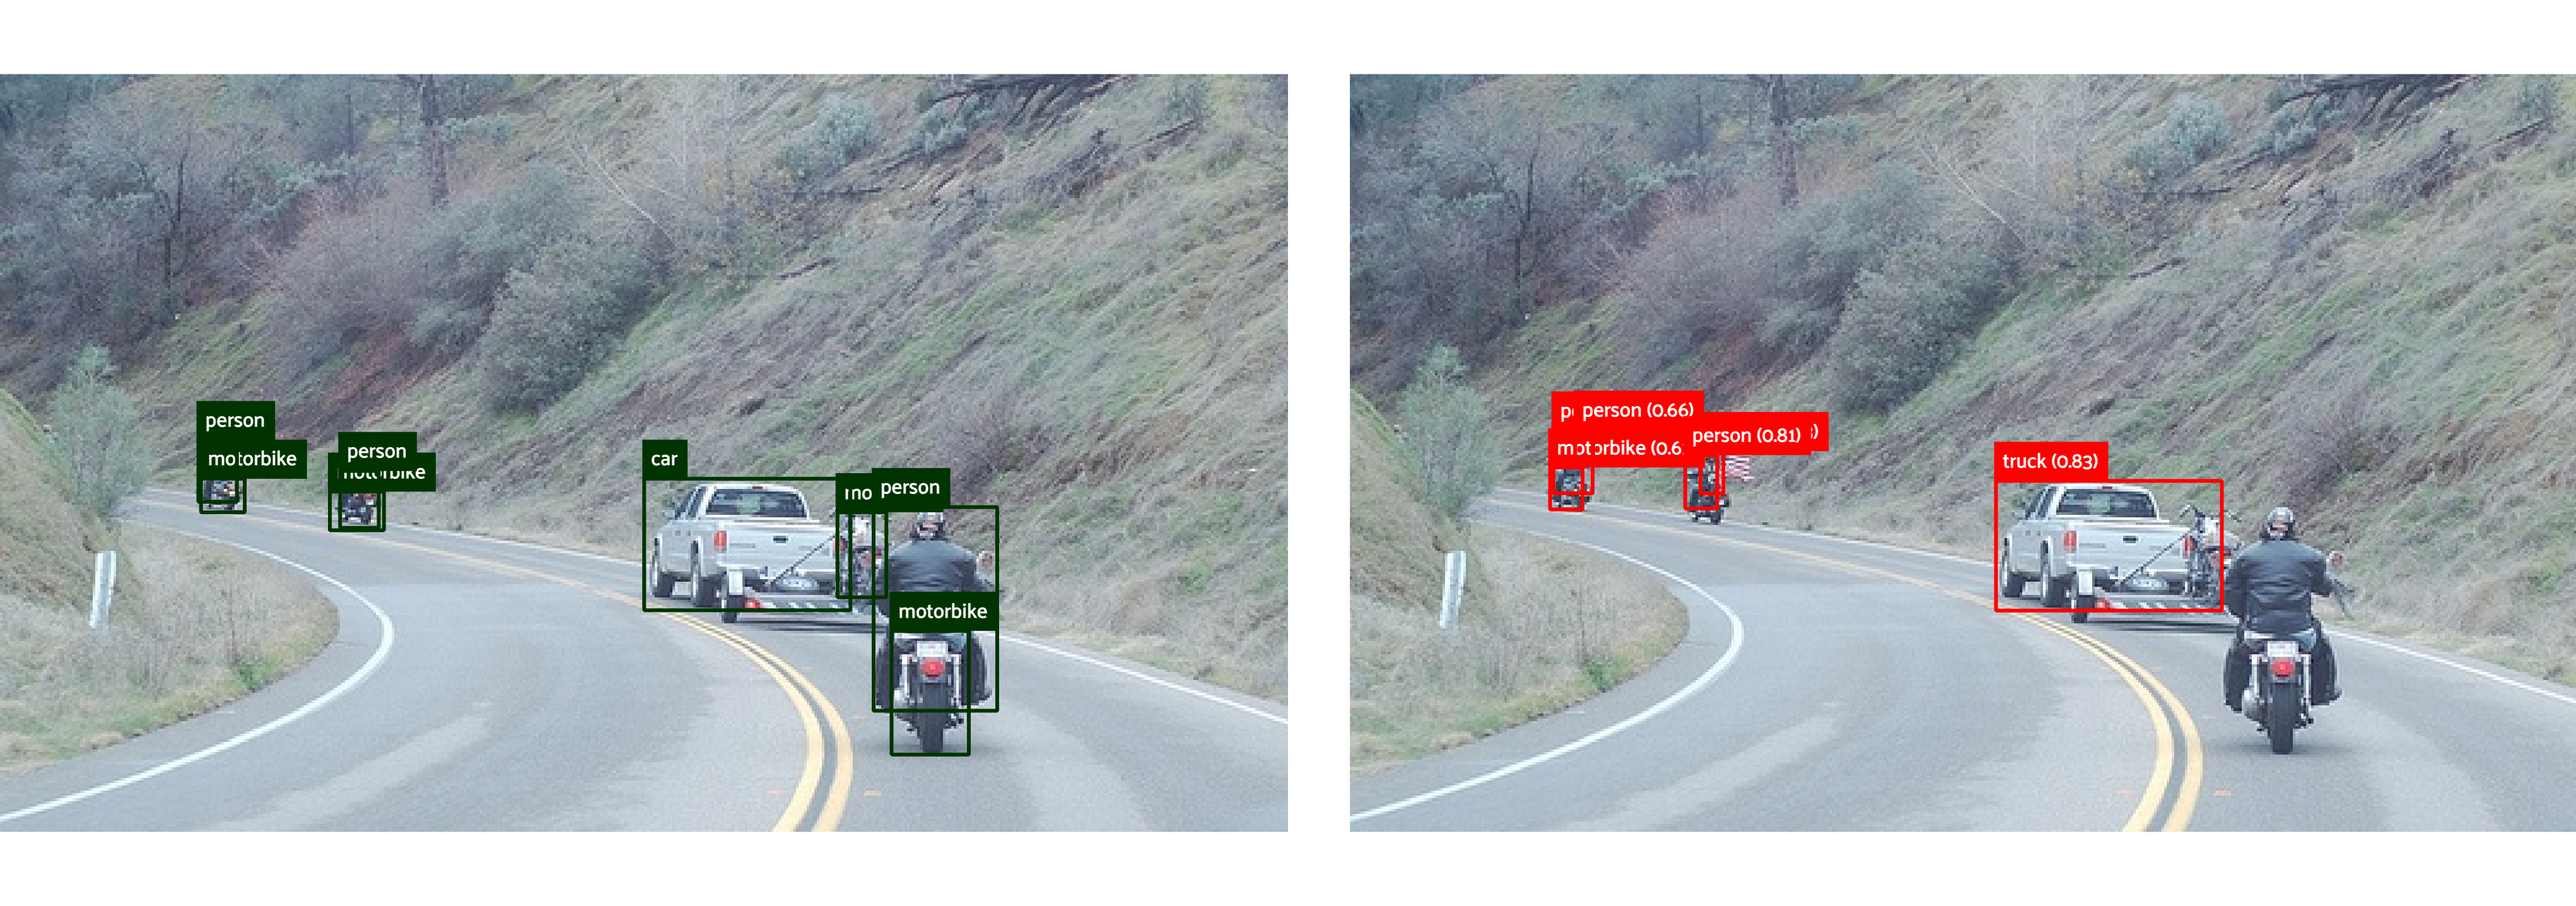
\includegraphics[width=0.5\textwidth]{images/rcnn_res/rcnn_b5.png}
    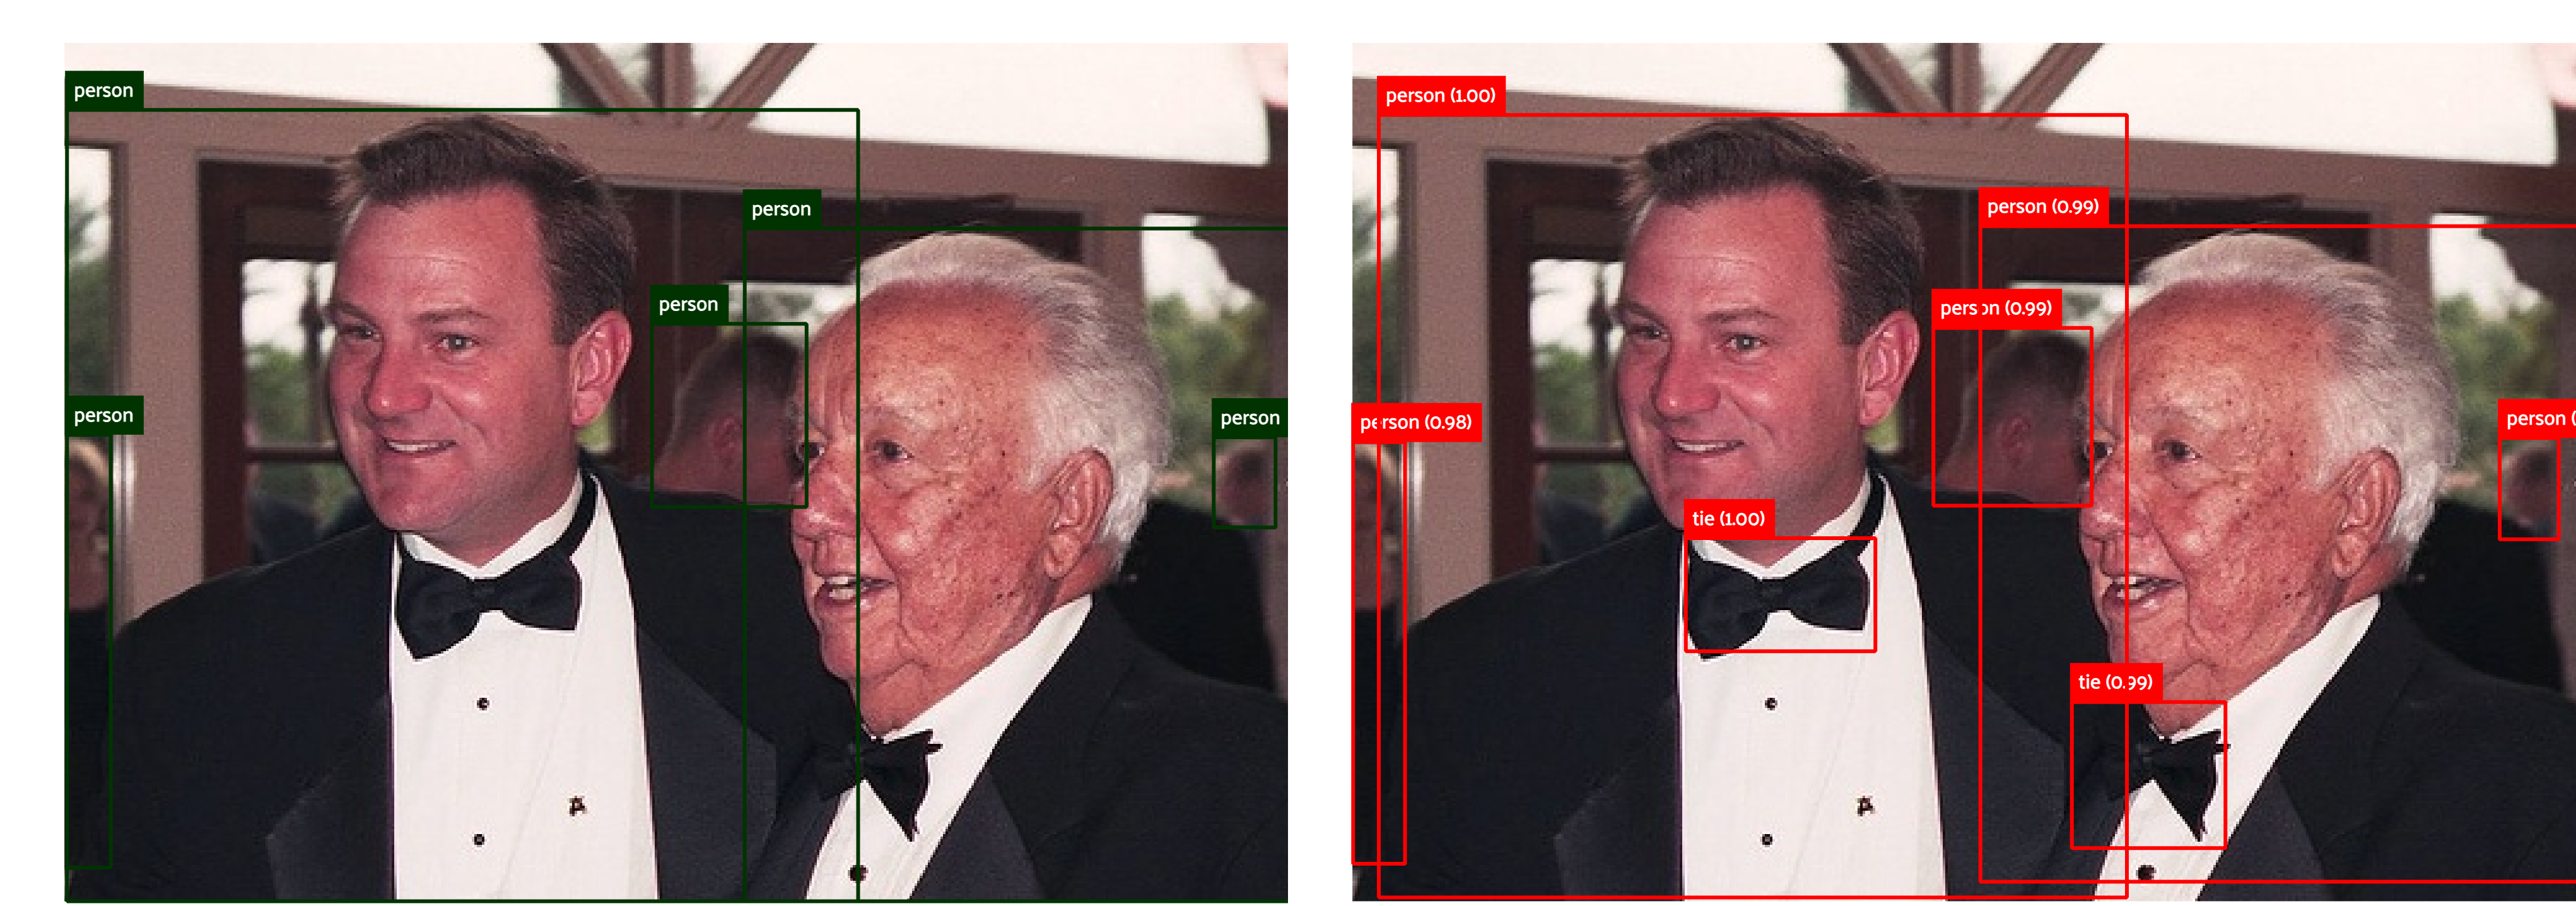
\includegraphics[width=0.5\textwidth]{images/rcnn_res/rcnn_b6.png}}
    \caption{Faster R-CNN Best Predictions}
    \label{fig:rcnn2}
\end{figure}

\begin{figure}[htbp]
    {\raggedright
    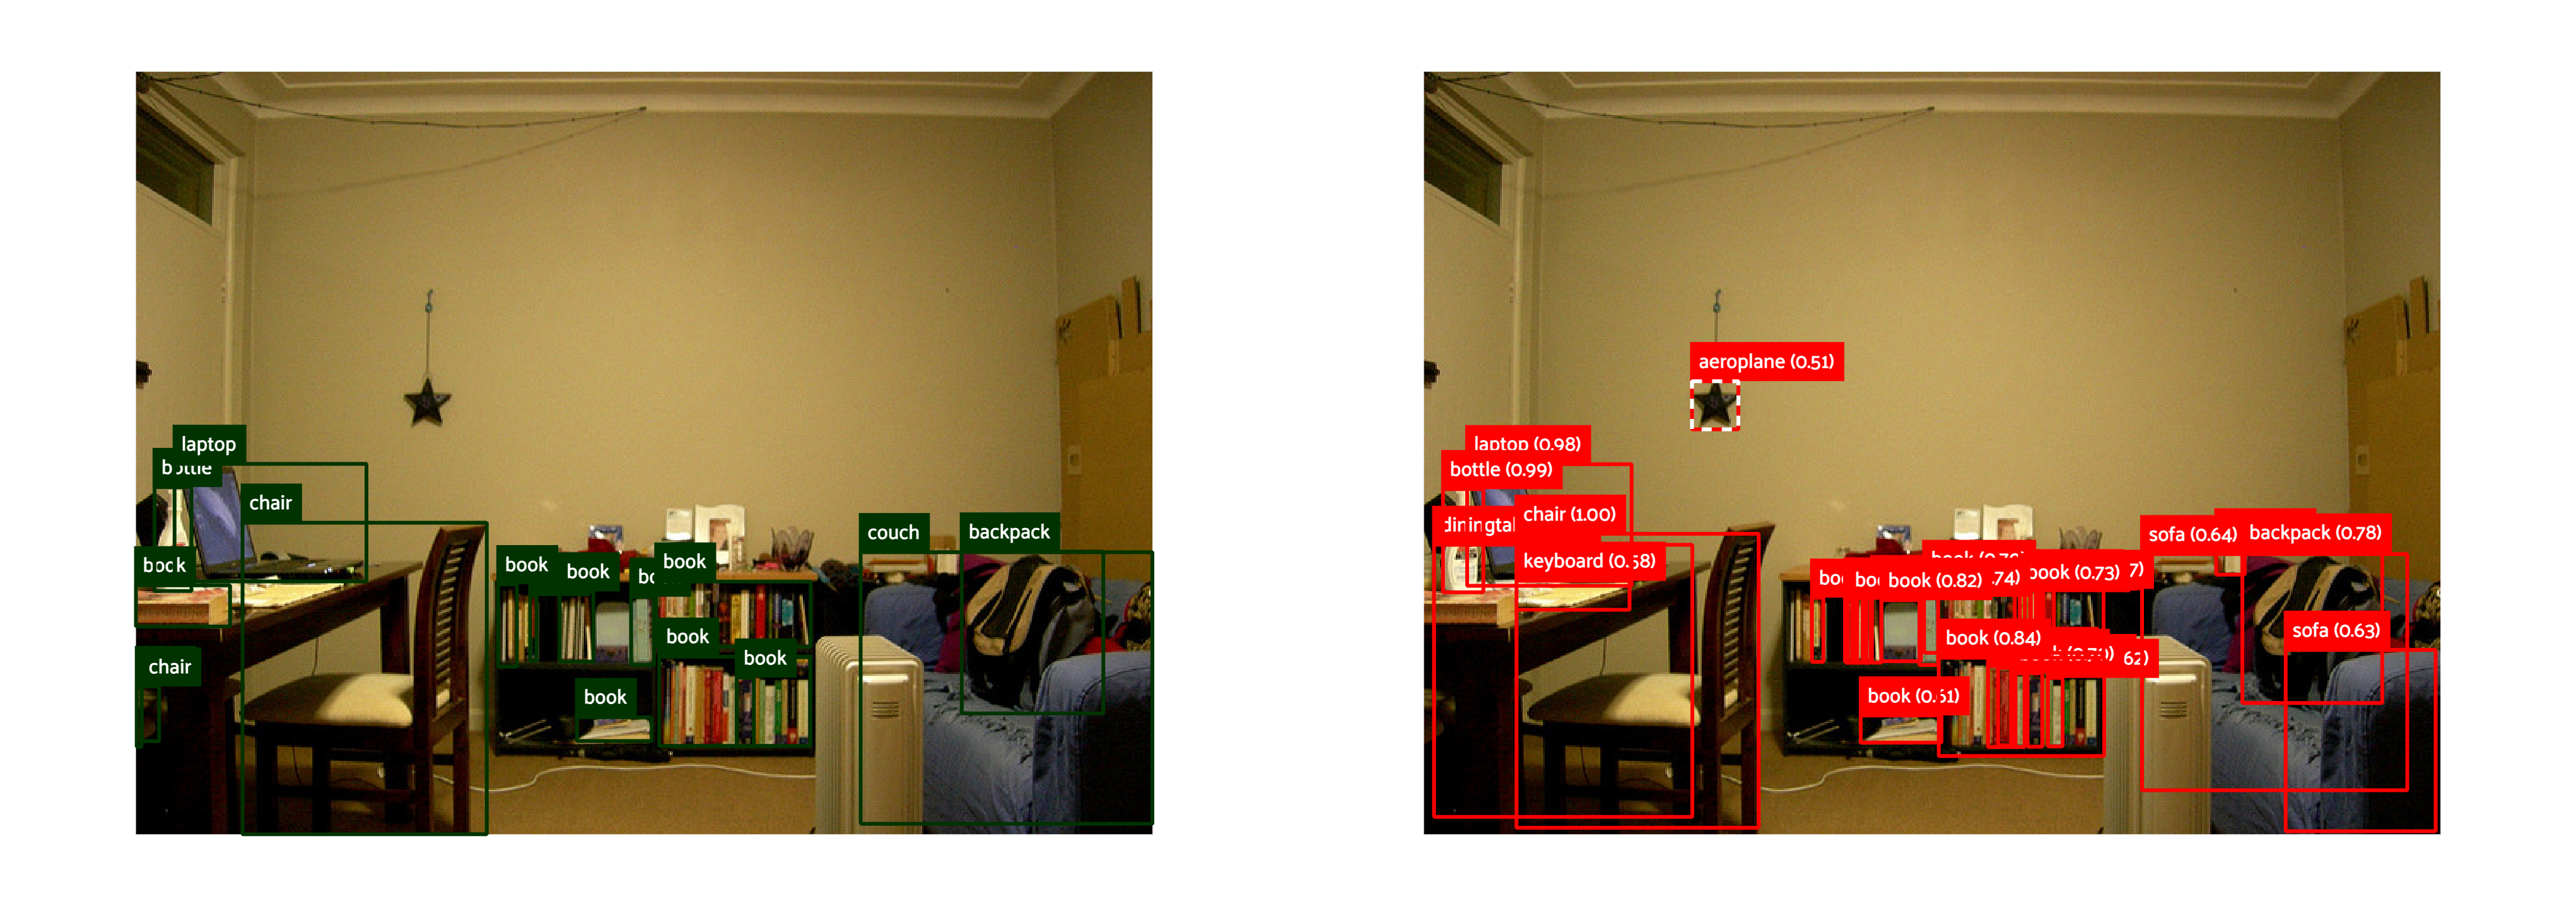
\includegraphics[width=0.5\textwidth]{images/rcnn_res/rcnn_w1.png}
    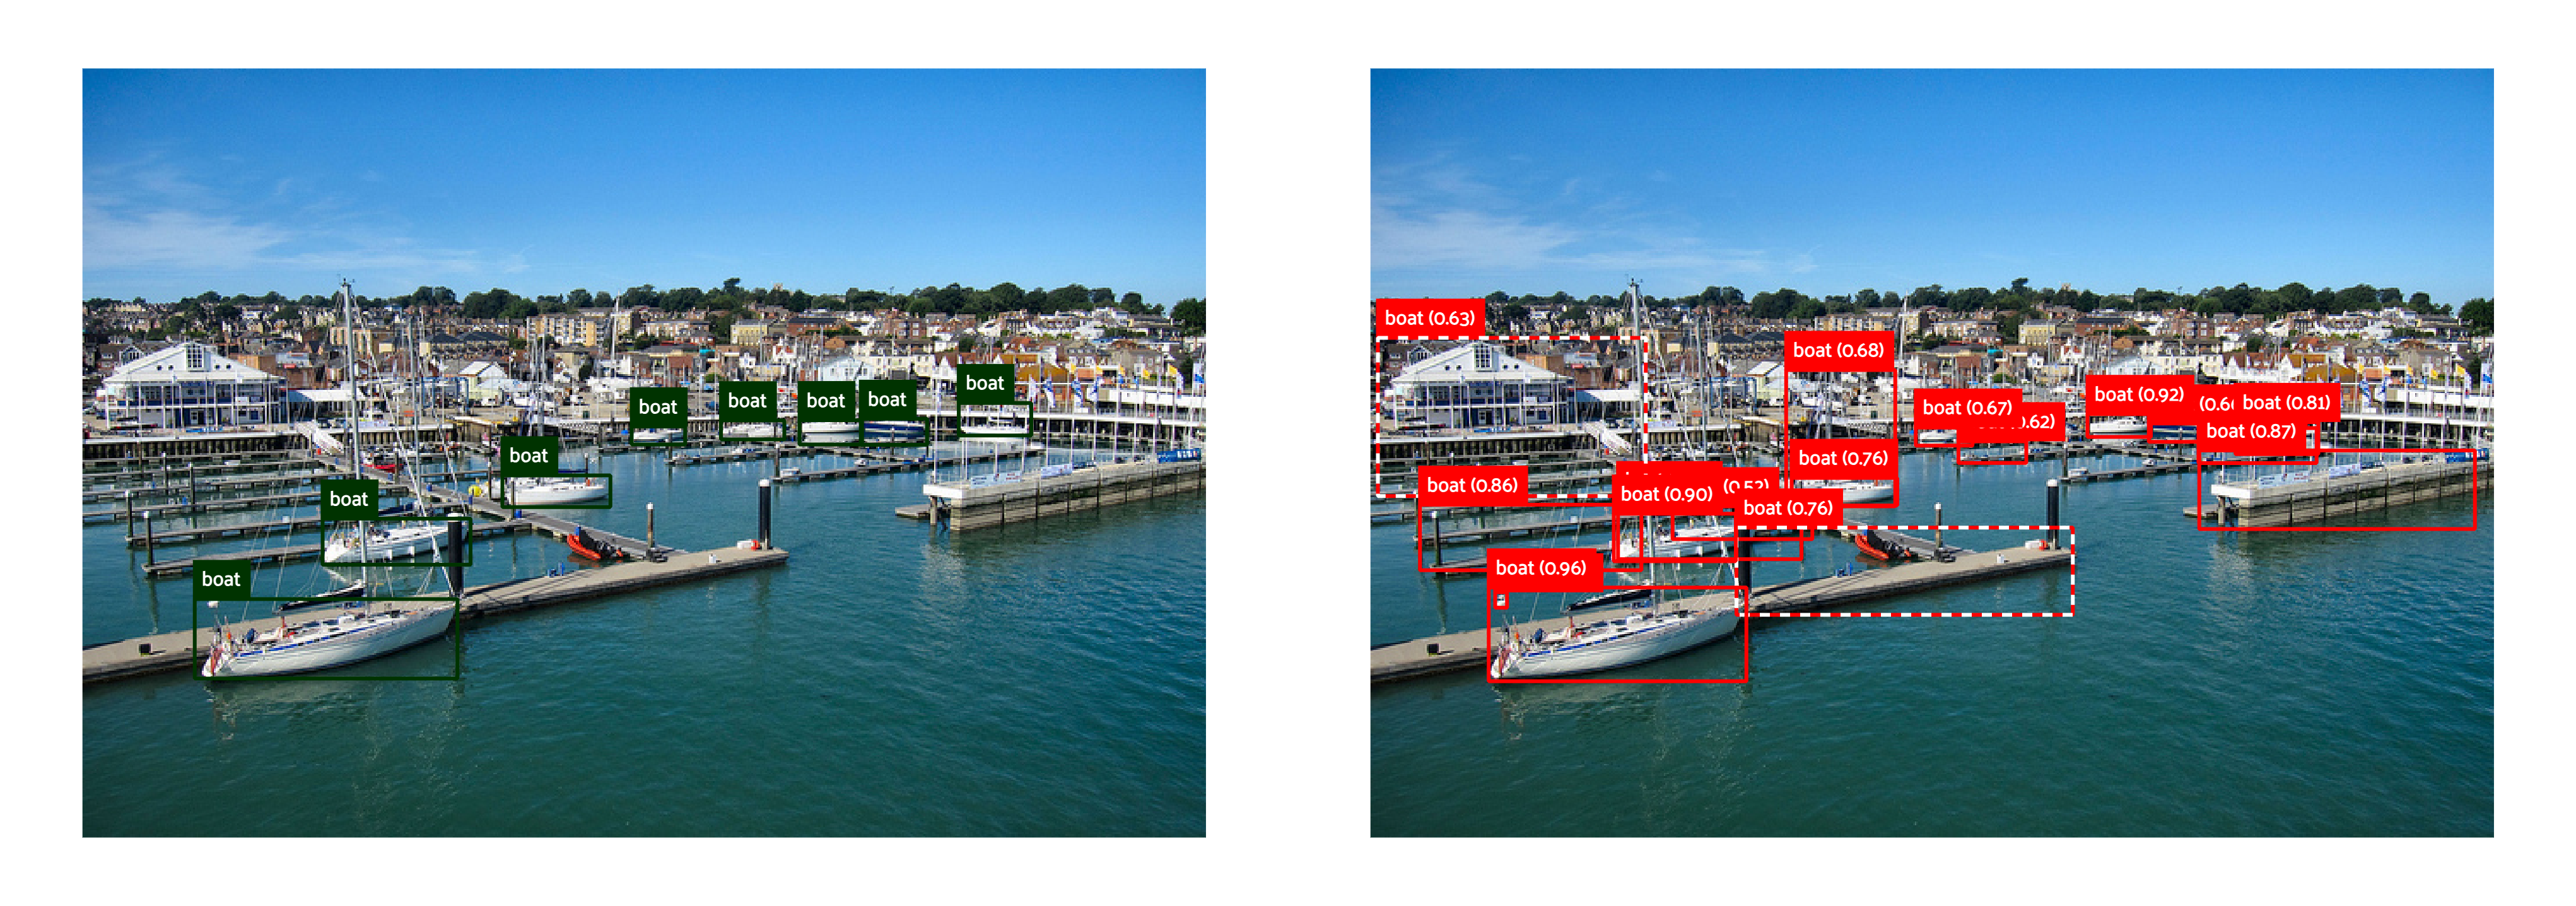
\includegraphics[width=0.5\textwidth]{images/rcnn_res/rcnn_w2.png}
    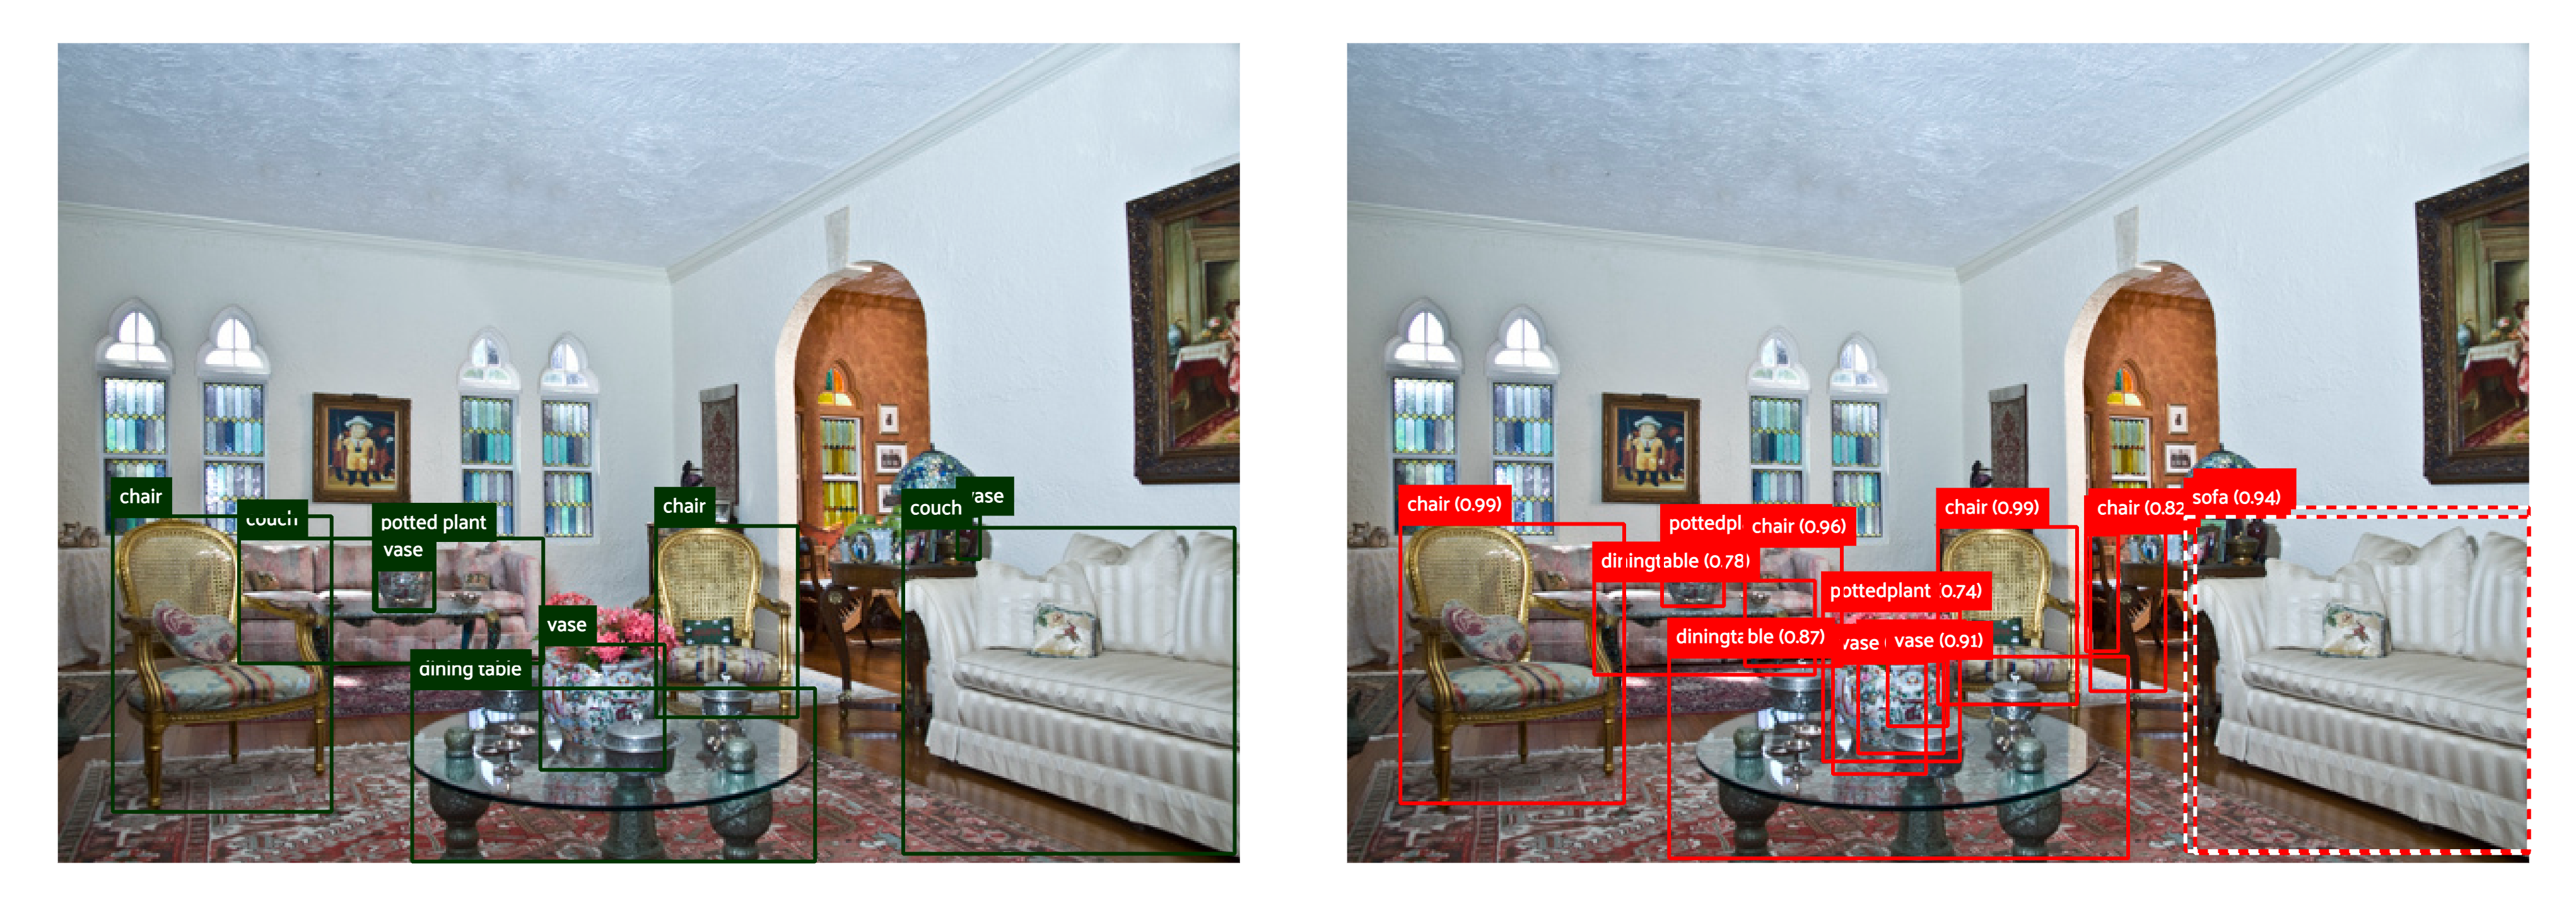
\includegraphics[width=0.5\textwidth]{images/rcnn_res/rcnn_w3.png}}
    {\raggedleft
    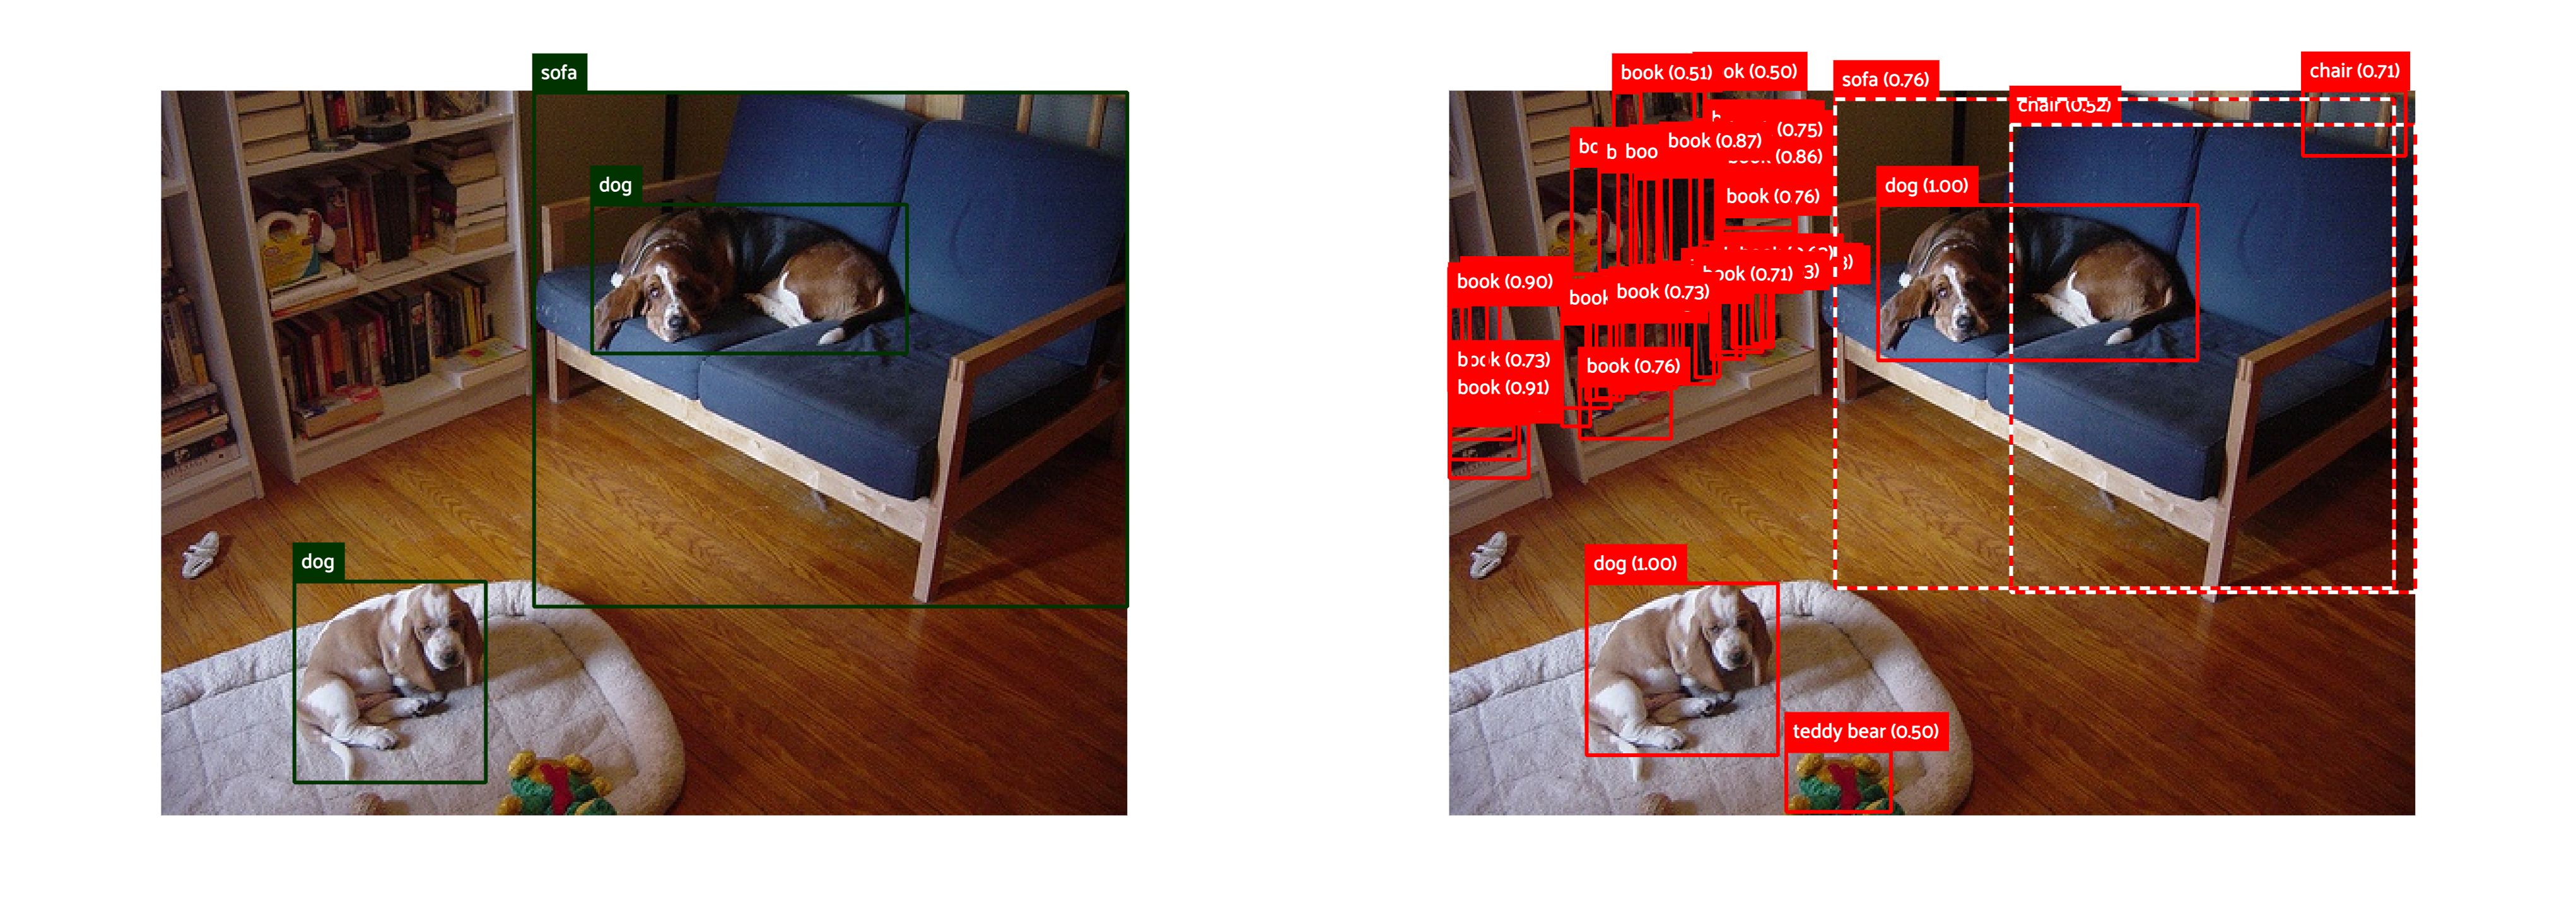
\includegraphics[width=0.5\textwidth]{images/rcnn_res/rcnn_w4.png}
    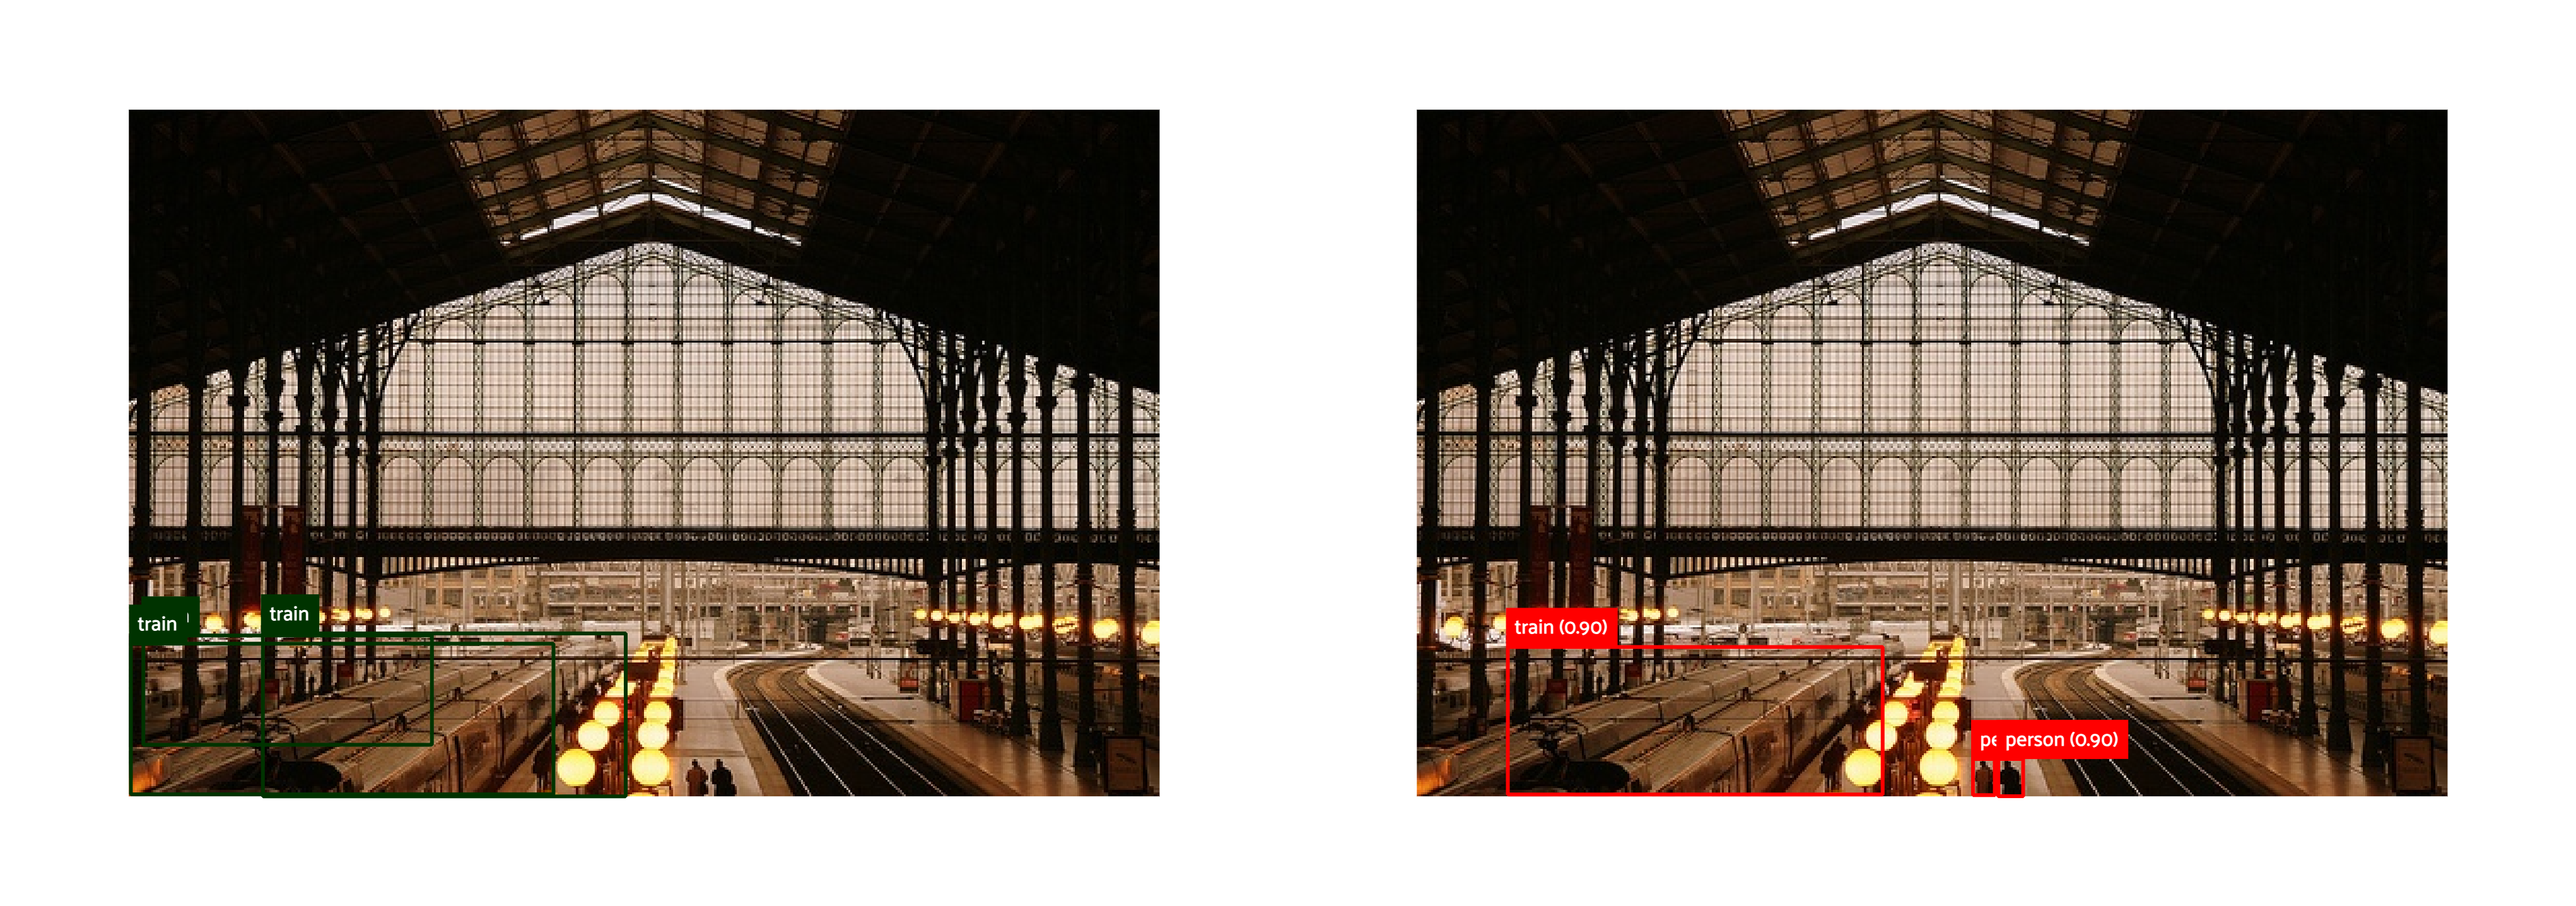
\includegraphics[width=0.5\textwidth]{images/rcnn_res/rcnn_w5.png}
    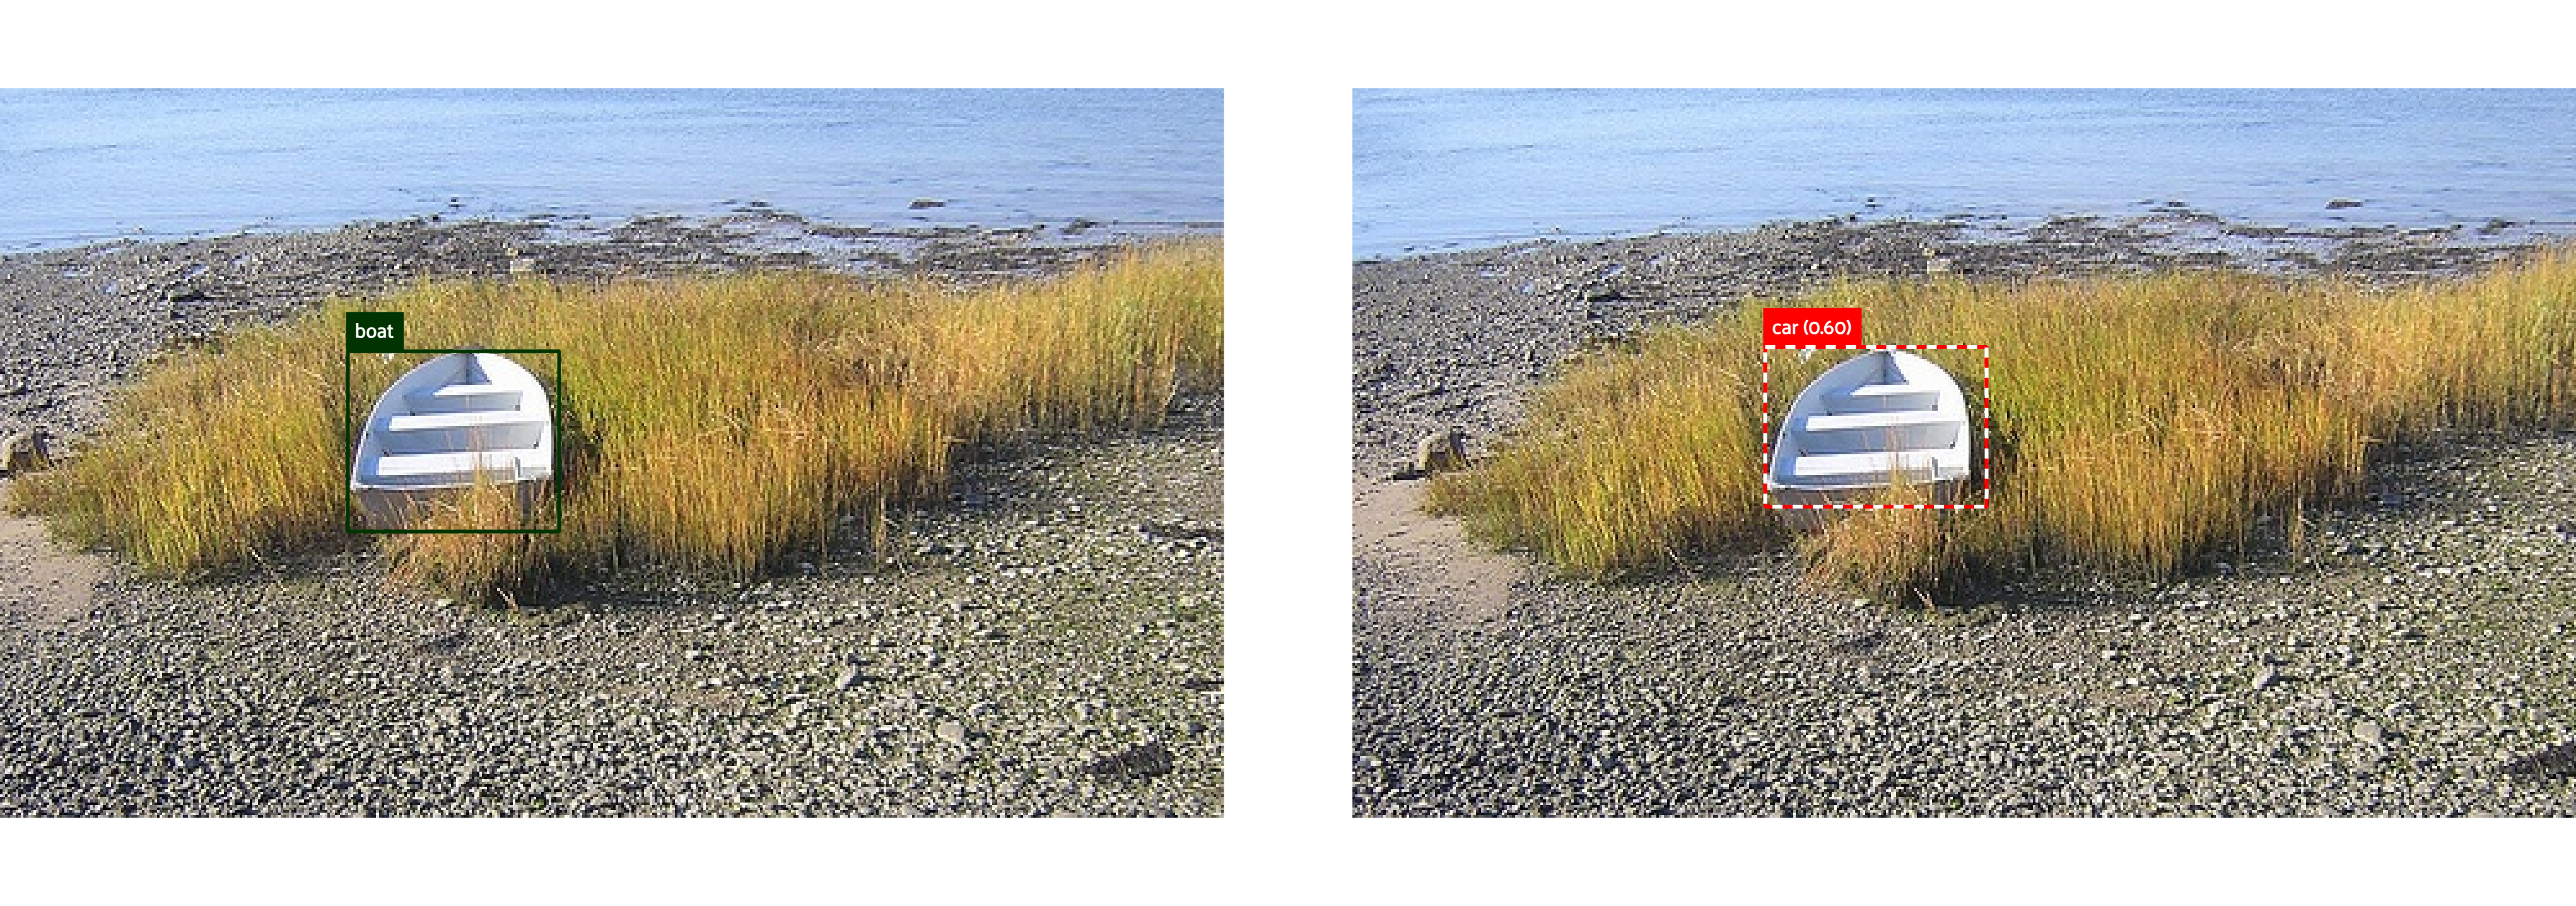
\includegraphics[width=0.5\textwidth]{images/rcnn_res/rcnn_w6.png}}
    \caption{Faster R-CNN Worst Predictions}
    \label{fig:rcnn3}
\end{figure}

Best predictions is at Figure \ref{fig:rcnn2}.
\\
Worst predictions is at Figure \ref{fig:rcnn3}.

\section{Retina Net}


\subsection{Introduction}
RetinaNet is one of the best one-stage object detection models that has proven to work well with dense and small scale objects. For this reason, it has become a popular object detection model to be used with aerial and satellite imagery.
\\
RetinaNet has been formed by making two improvements over existing single stage object detection models - Feature Pyramid Networks (FPN) and Focal Loss.
\subsection{Architecture}
\begin{figure}[h]
    \centering
    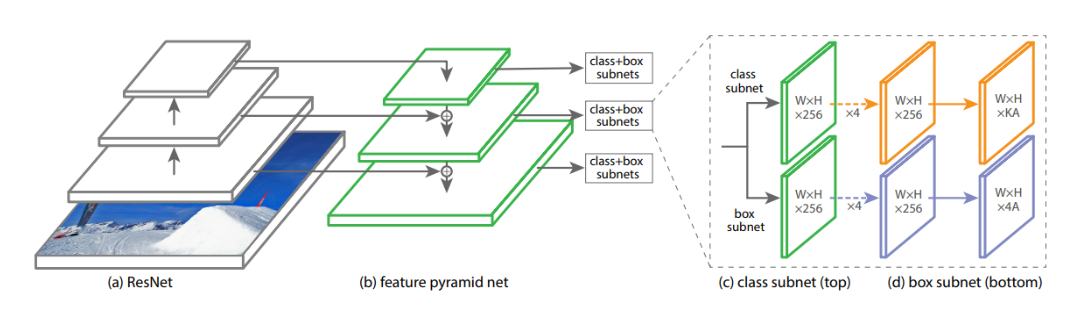
\includegraphics[width=0.75\textwidth]{images/retina_arch.png}
    \caption{Retina Net Architecture}
    \label{fig:retina1}
\end{figure}

\paragraph{There are four major components of a RetinaNet model architecture:}

\begin{enumerate}[leftmargin=1cm, labelwidth=4cm]
  \item Bottom-up Pathway - The backbone network (e.g. ResNet) which calculates the feature maps at different scales, irrespective of the input image size or the backbone.
  \item Top-down pathway and Lateral connections - The top down pathway upsamples the spatially coarser feature maps from higher pyramid levels, and the lateral connections merge the top-down layers and the bottom-up layers with the same spatial size.
  \item Classification subnetwork - It predicts the probability of an object being present at each spatial location for each anchor box and object class.
  \item Regression subnetwork - It's regresses the offset for the bounding boxes from the anchor boxes for each ground-truth object
\end{enumerate}


\paragraph{Focal Loss (FL)}
 is an enhancement over Cross-Entropy Loss (CE) and is introduced to handle the class imbalance problem with single-stage object detection models. Single Stage models suffer from a extreme foreground-background class imbalance problem. In RetinaNet, at each pyramid layer there can be thousands of anchor boxes. Only a few will be assigned to a ground-truth object while the vast majority will be background class. These easy examples (detections with high probabilities) although resulting in small loss values can collectively overwhelm the model. Focal Loss reduces the loss contribution from easy examples and increases the importance of correcting miss classified examples.

\subsection{Inference Results}

\begin{figure}[htbp]
    {\raggedright
    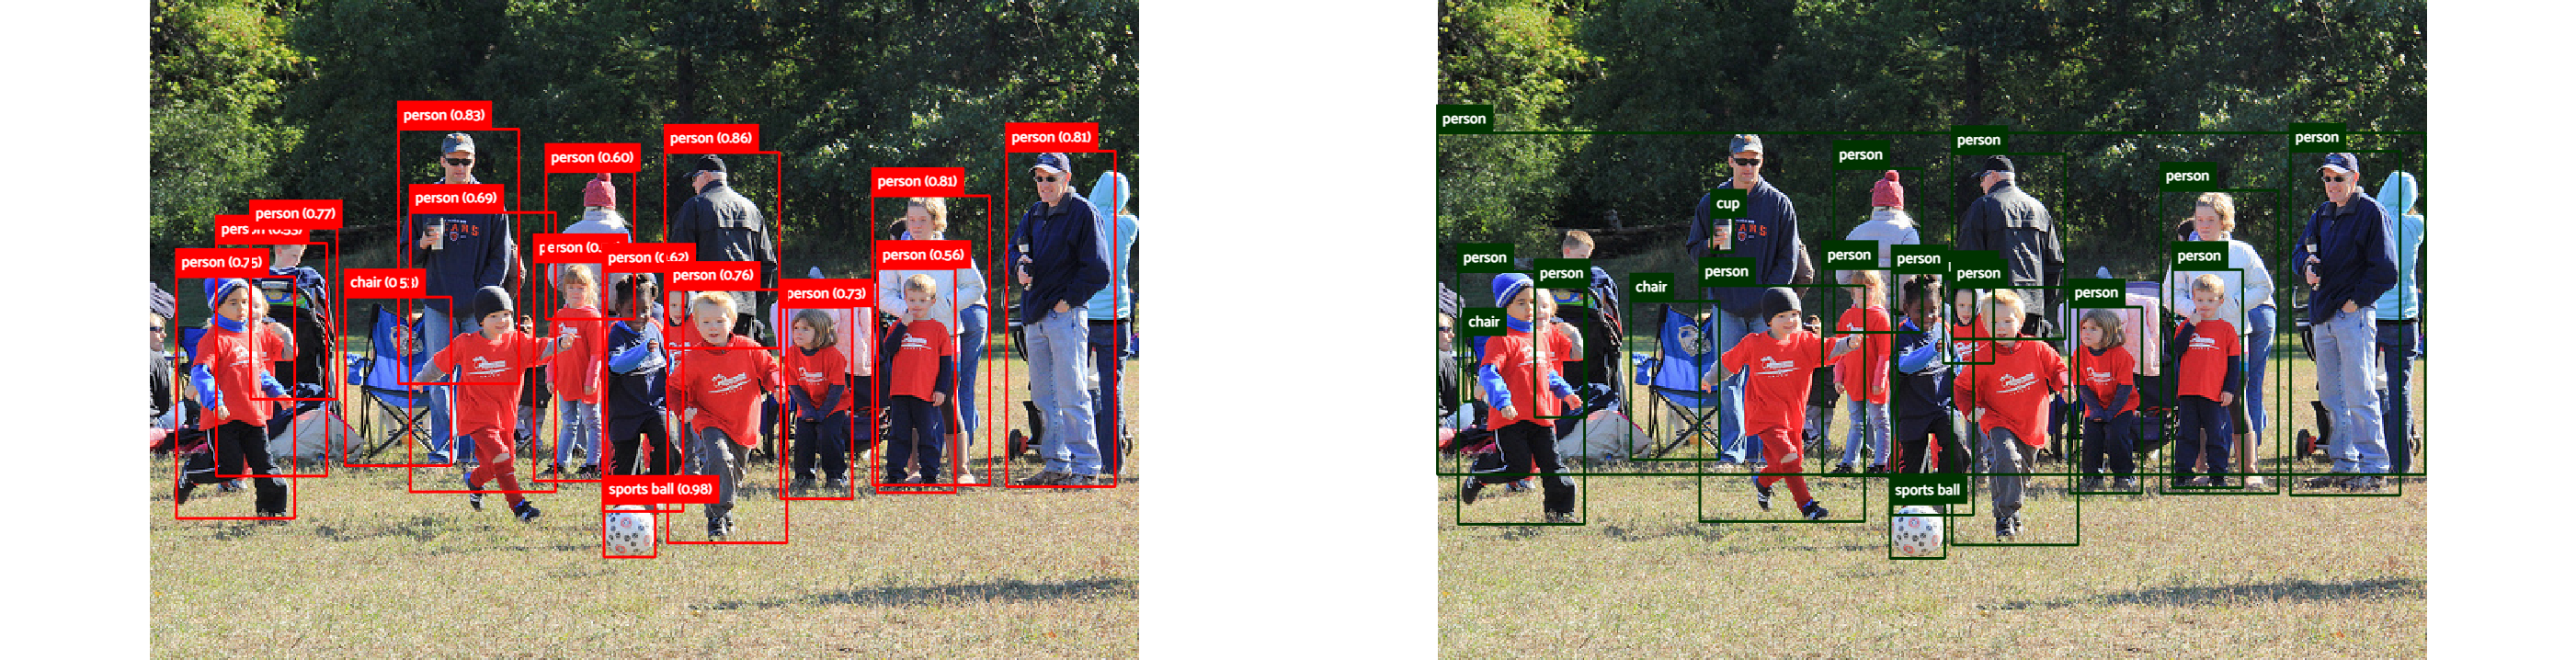
\includegraphics[width=0.5\textwidth]{images/retina_res/retina_b1.png}
    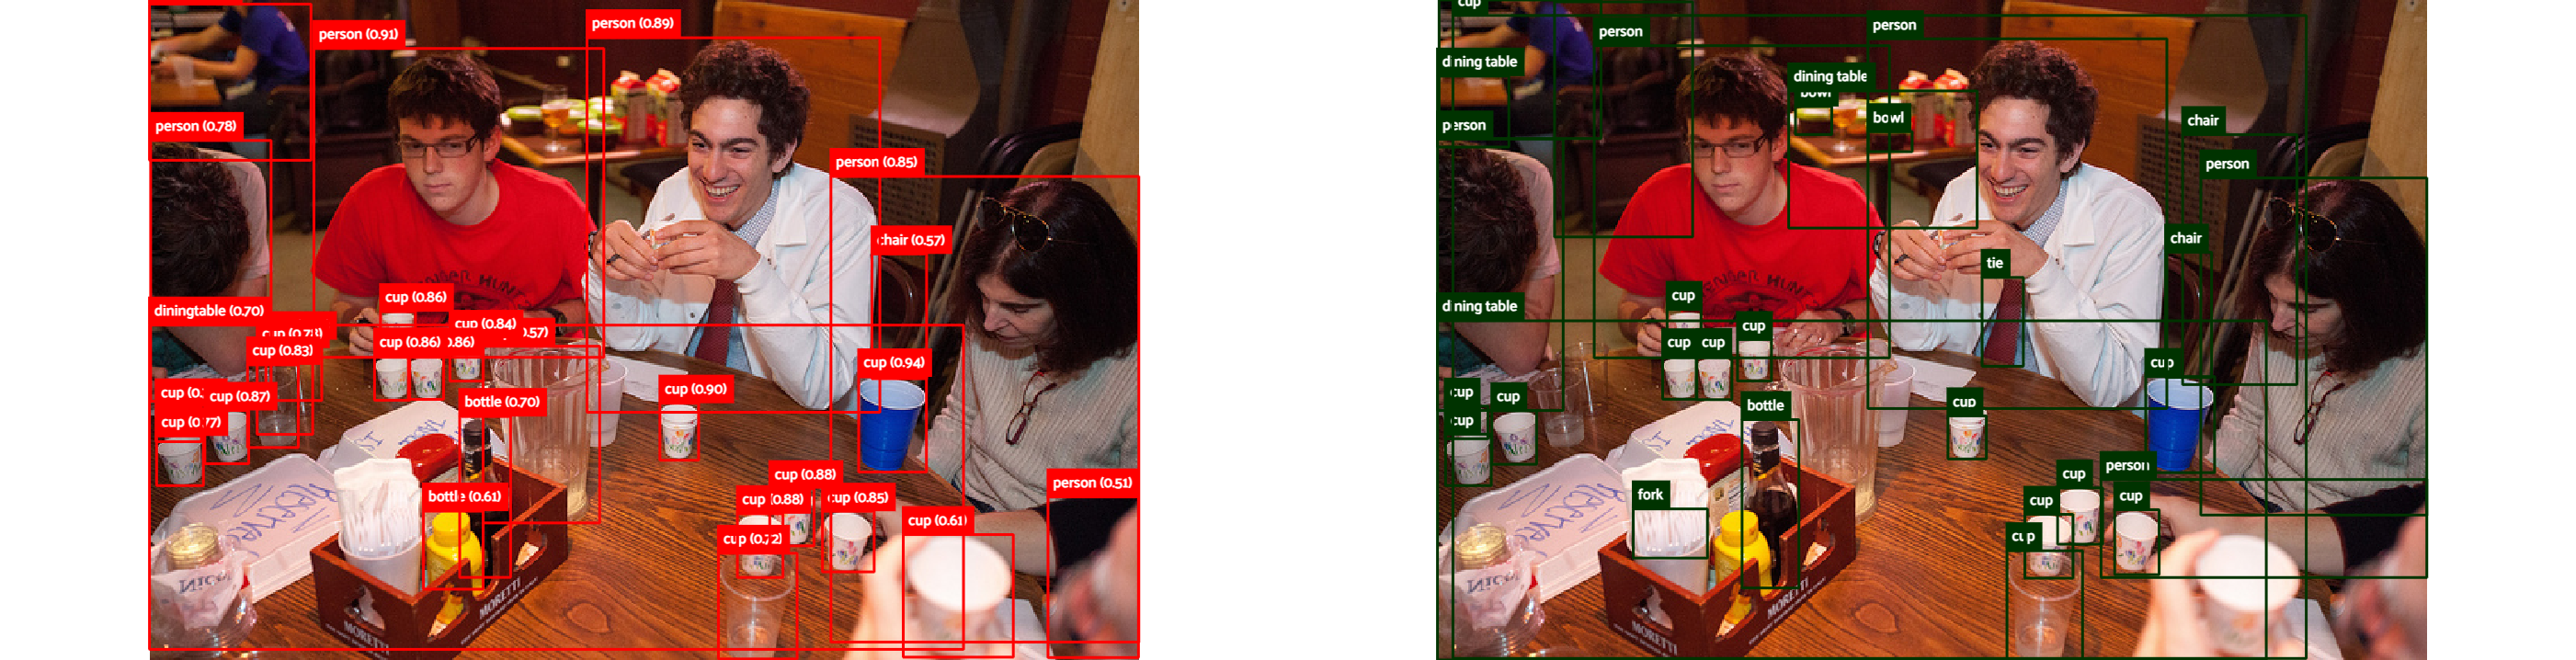
\includegraphics[width=0.5\textwidth]{images/retina_res/retina_b2.png}
    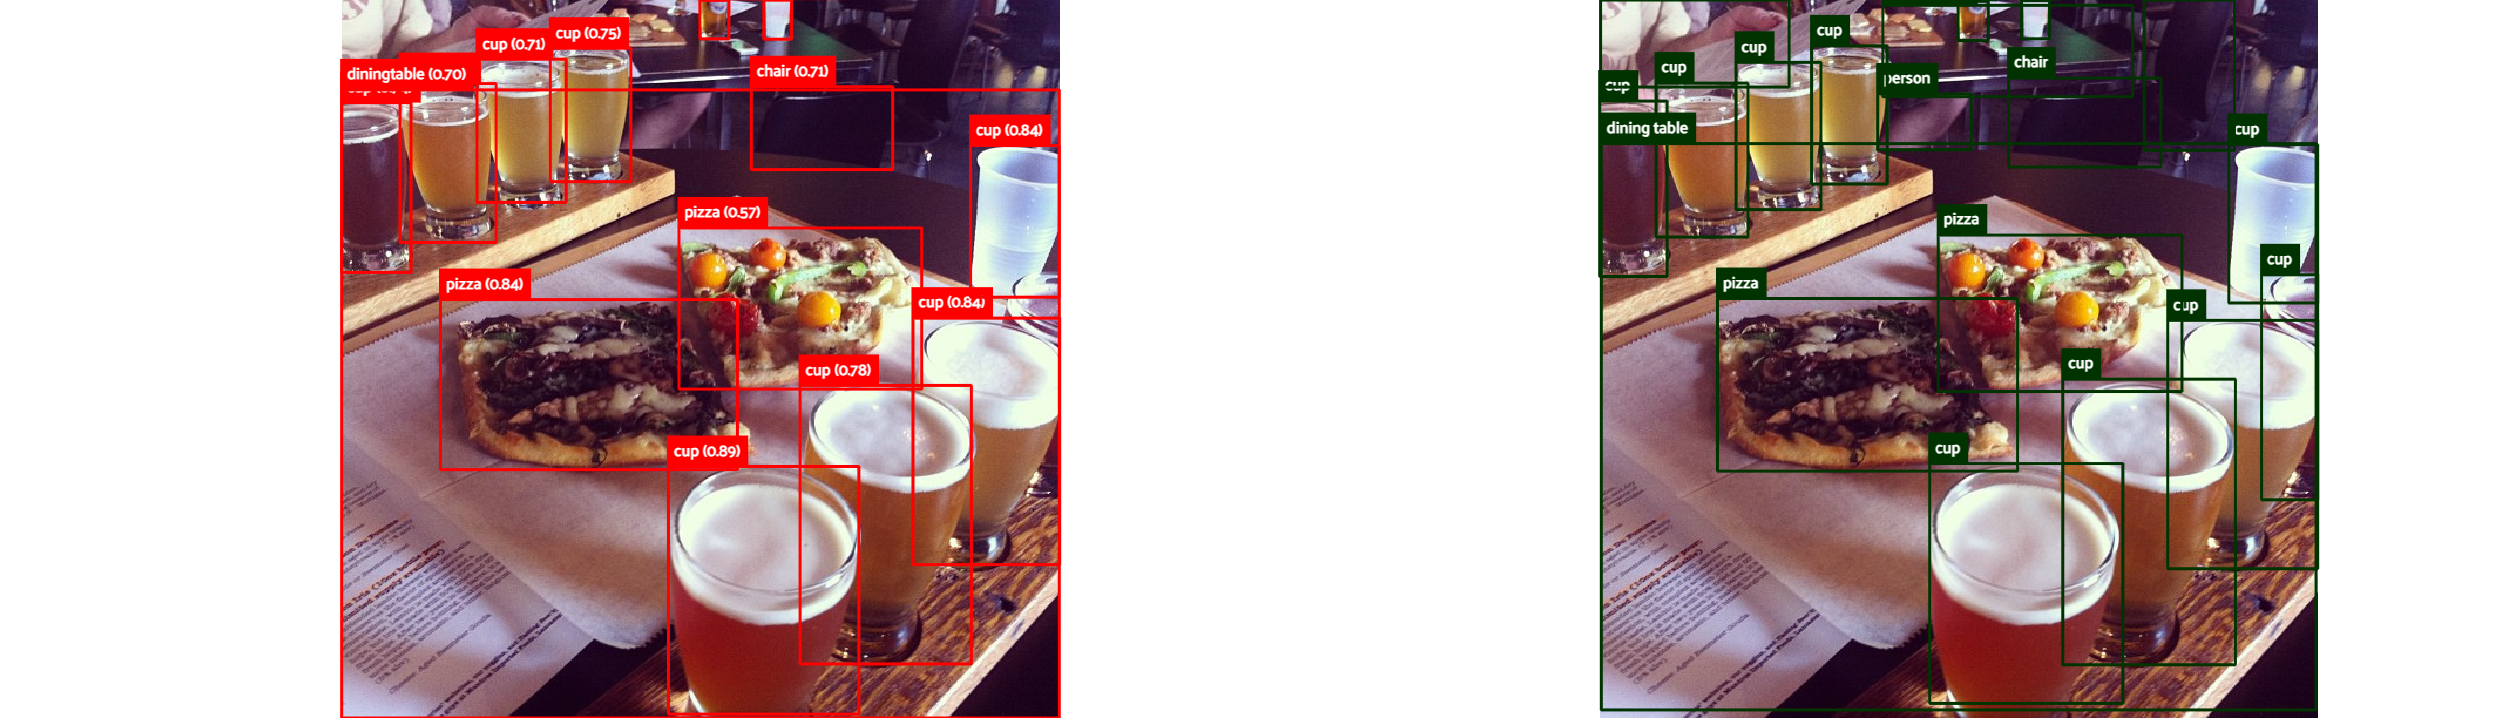
\includegraphics[width=0.5\textwidth]{images/retina_res/retina_b3.png}}
    {\raggedleft
    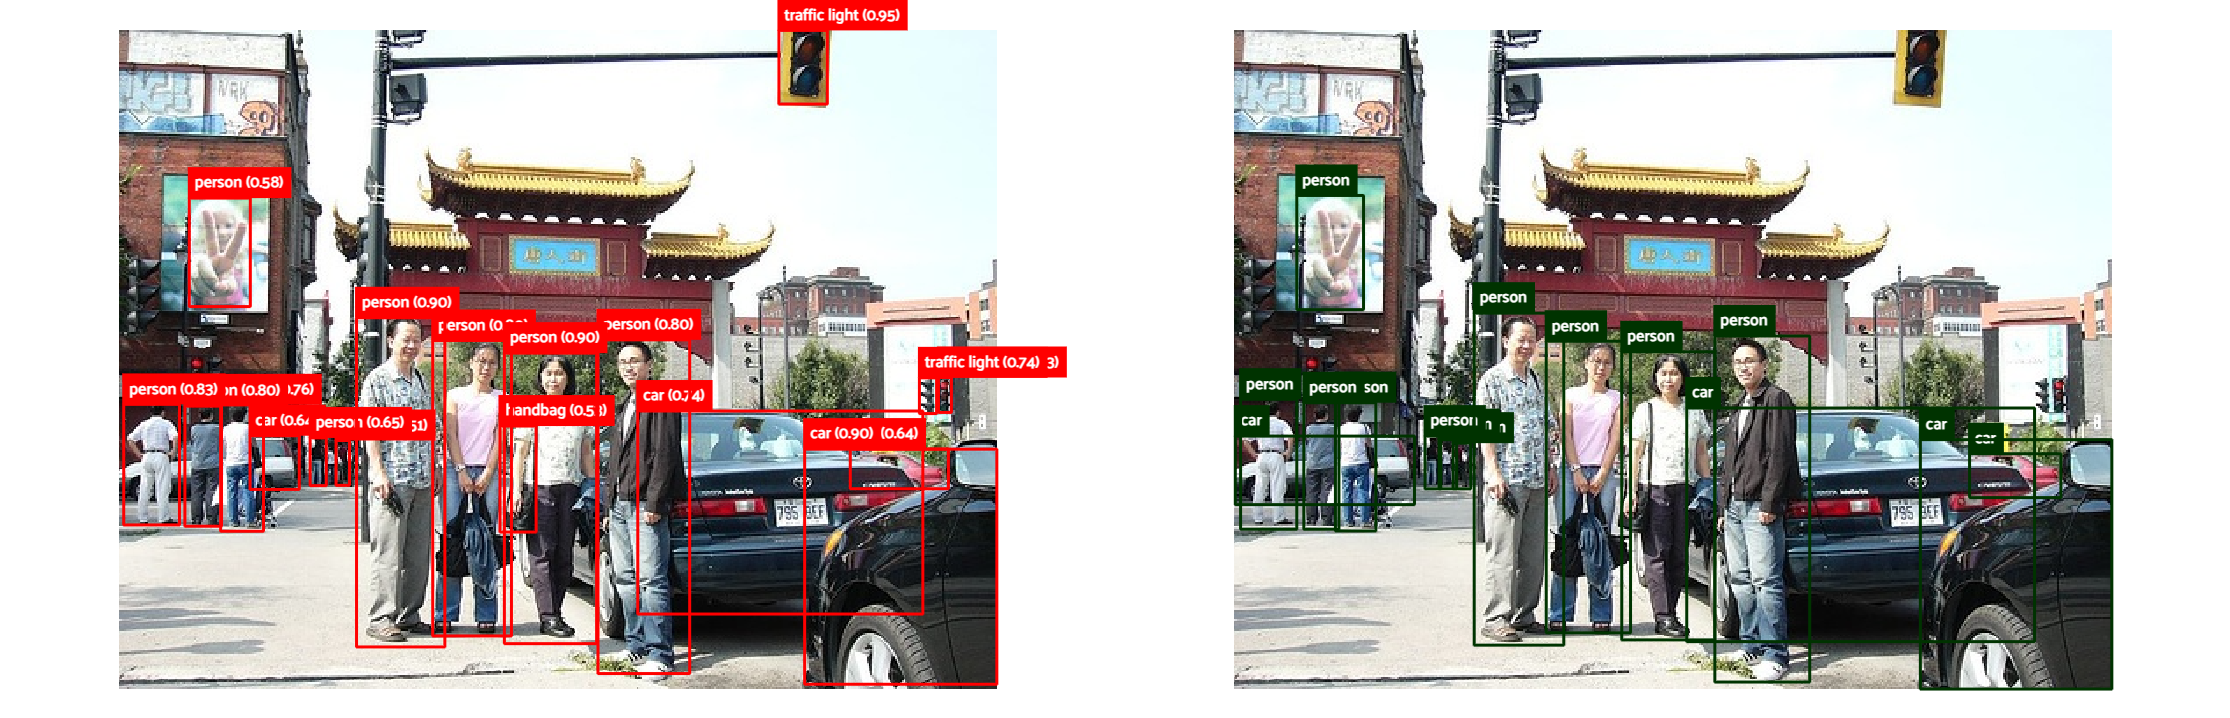
\includegraphics[width=0.5\textwidth]{images/retina_res/retina_b4.png}
    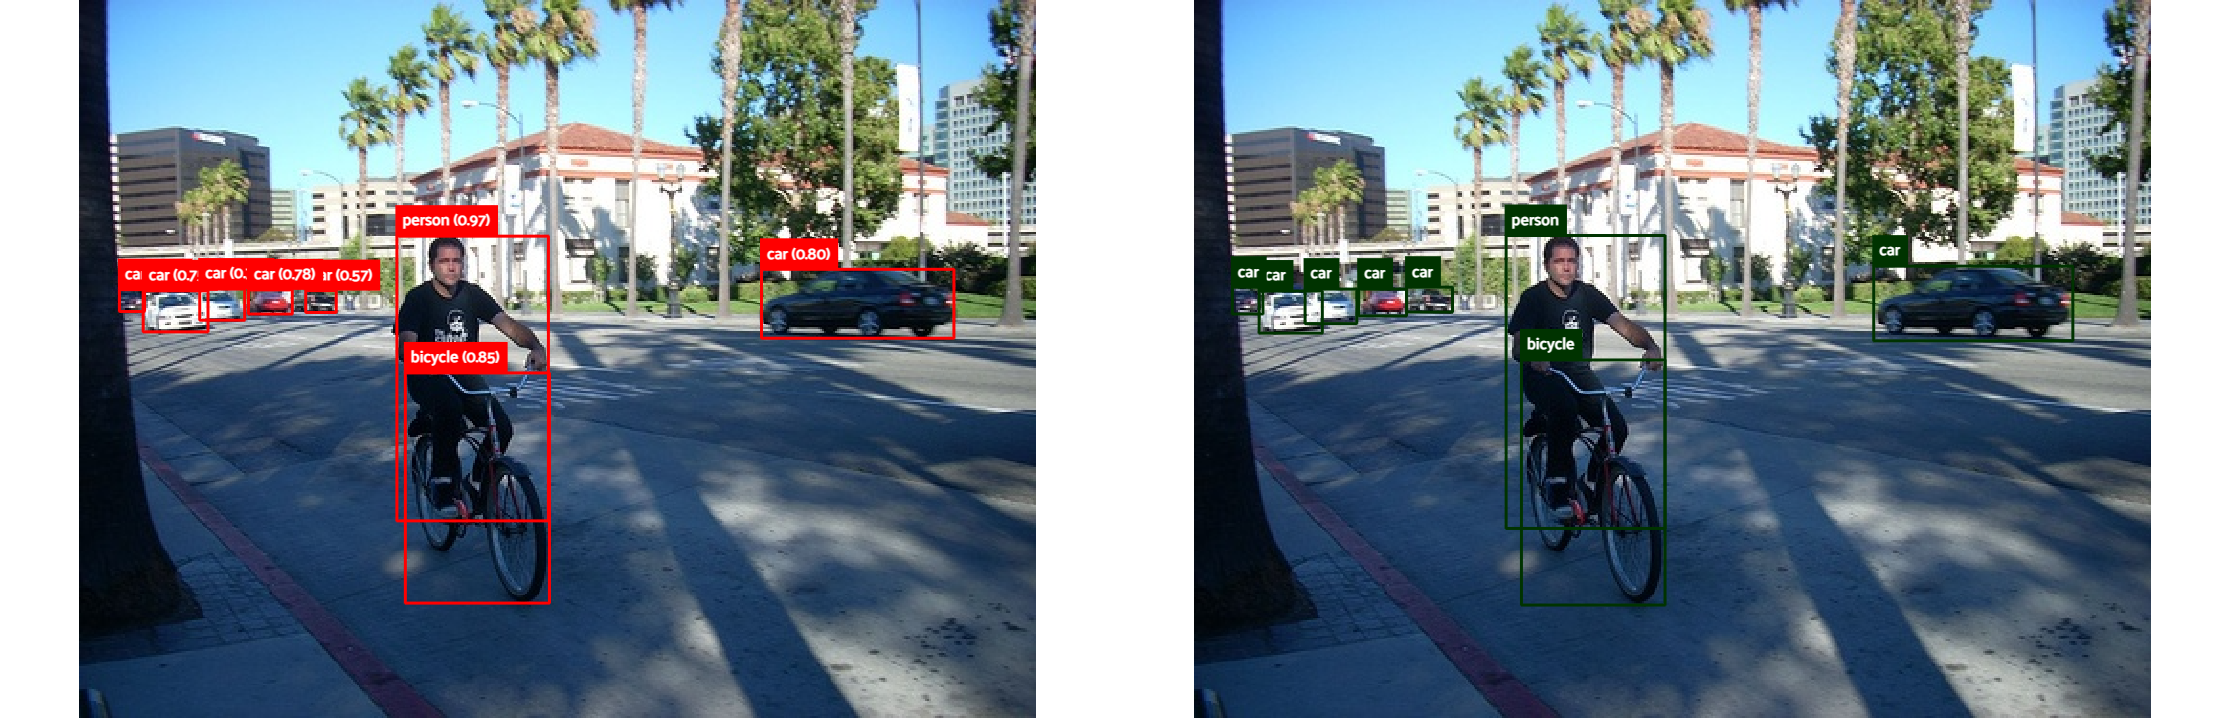
\includegraphics[width=0.5\textwidth]{images/retina_res/retina_b5.png}
    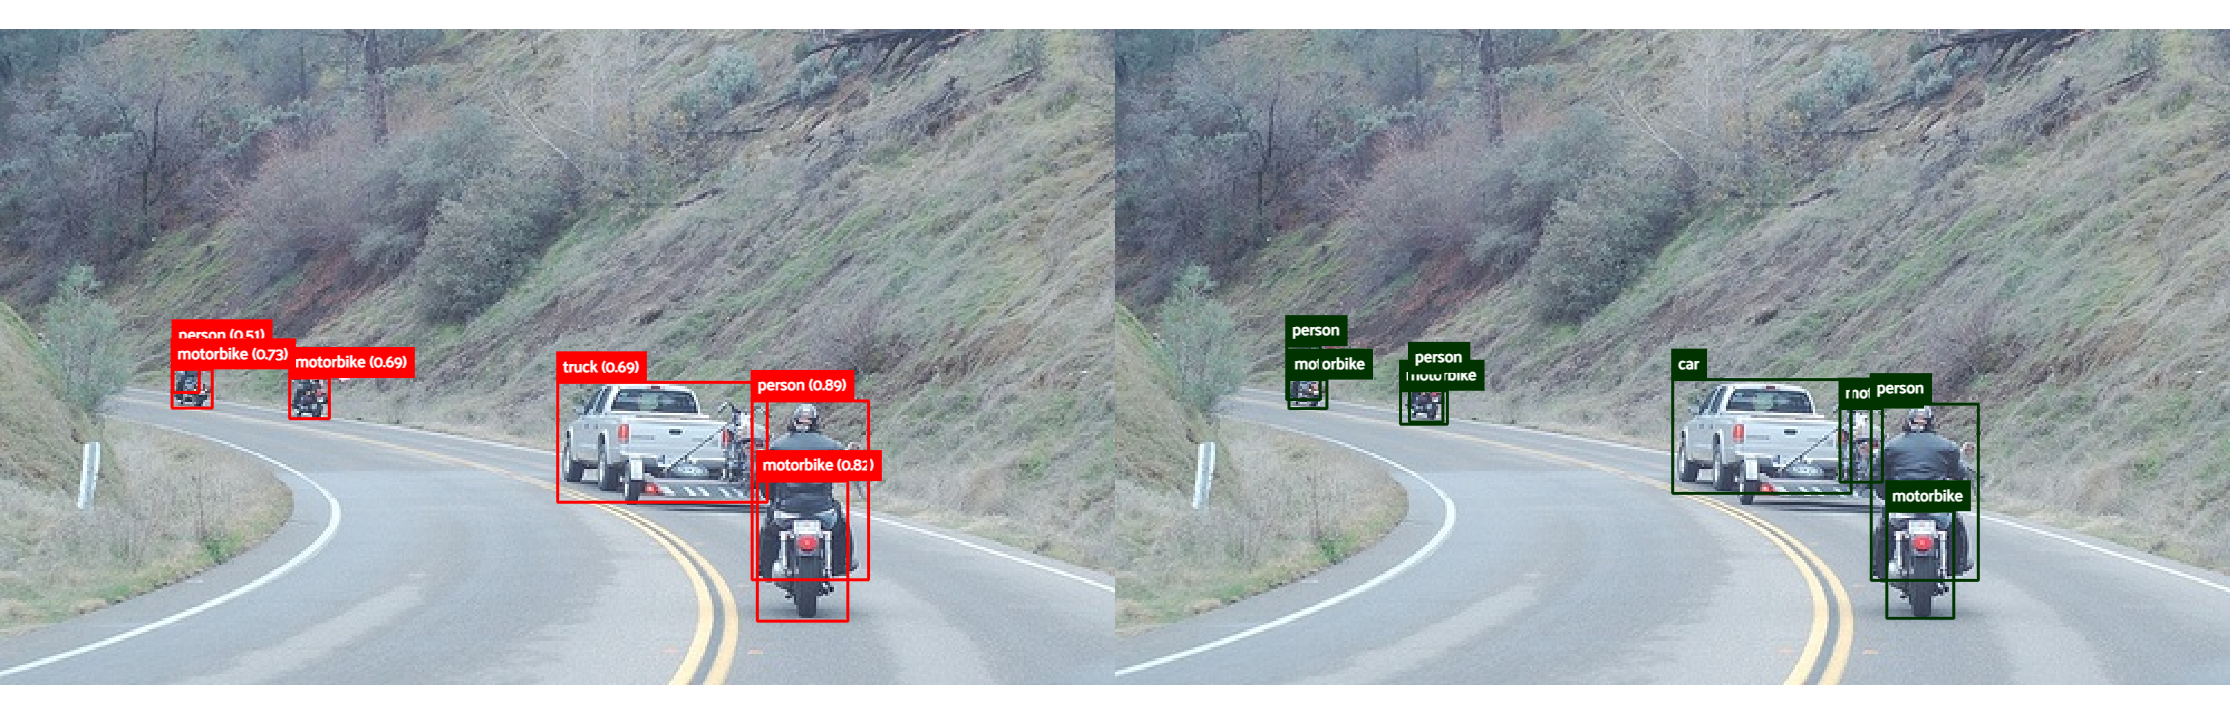
\includegraphics[width=0.5\textwidth]{images/retina_res/retina_b6.png}}
    \caption{Retina Net Best Predictions}
    \label{fig:retina2}
\end{figure}

\begin{figure}[htbp]
    {\raggedright
    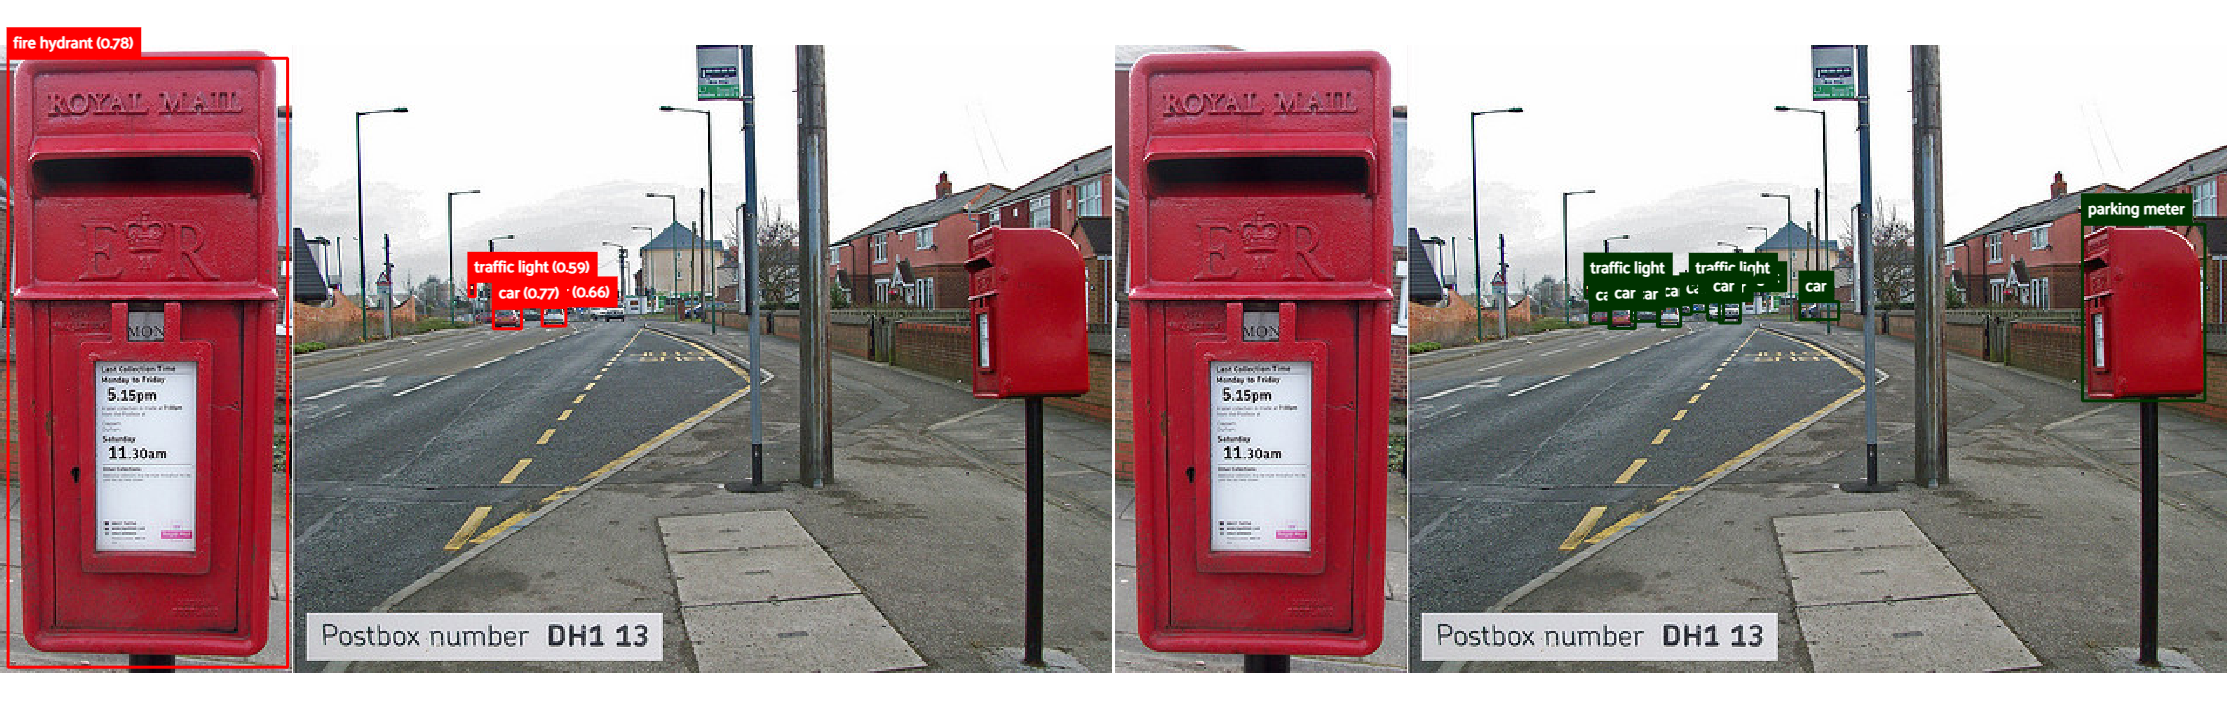
\includegraphics[width=0.5\textwidth]{images/retina_res/retina_w1.png}
    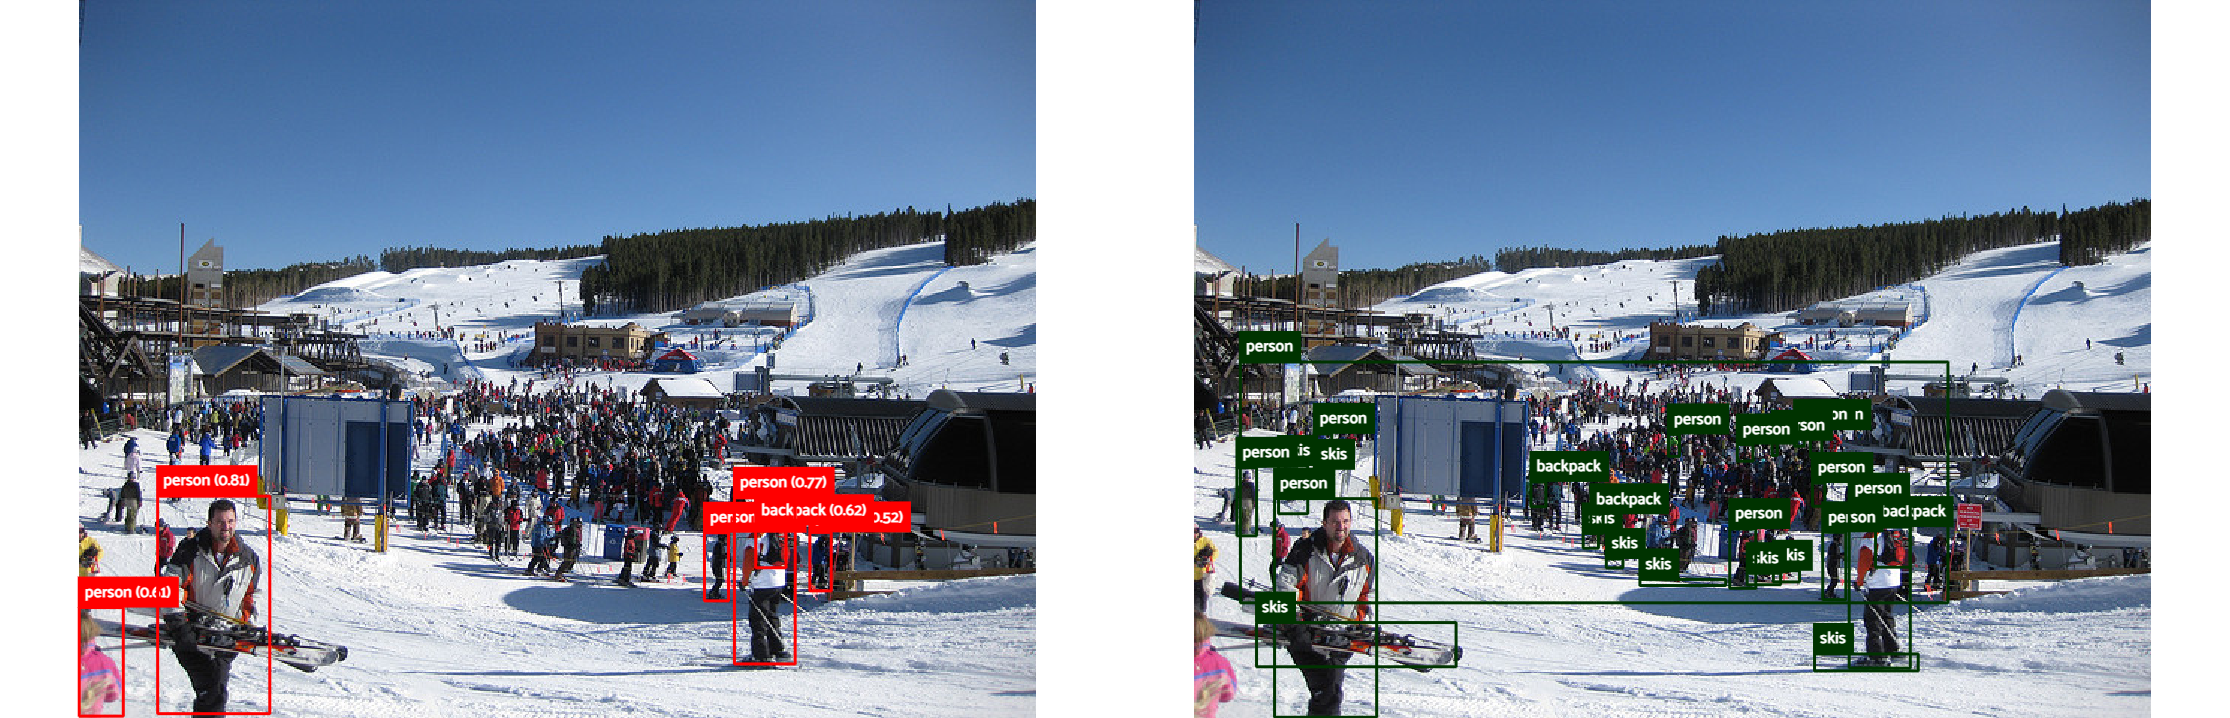
\includegraphics[width=0.5\textwidth]{images/retina_res/retina_w2.png}
    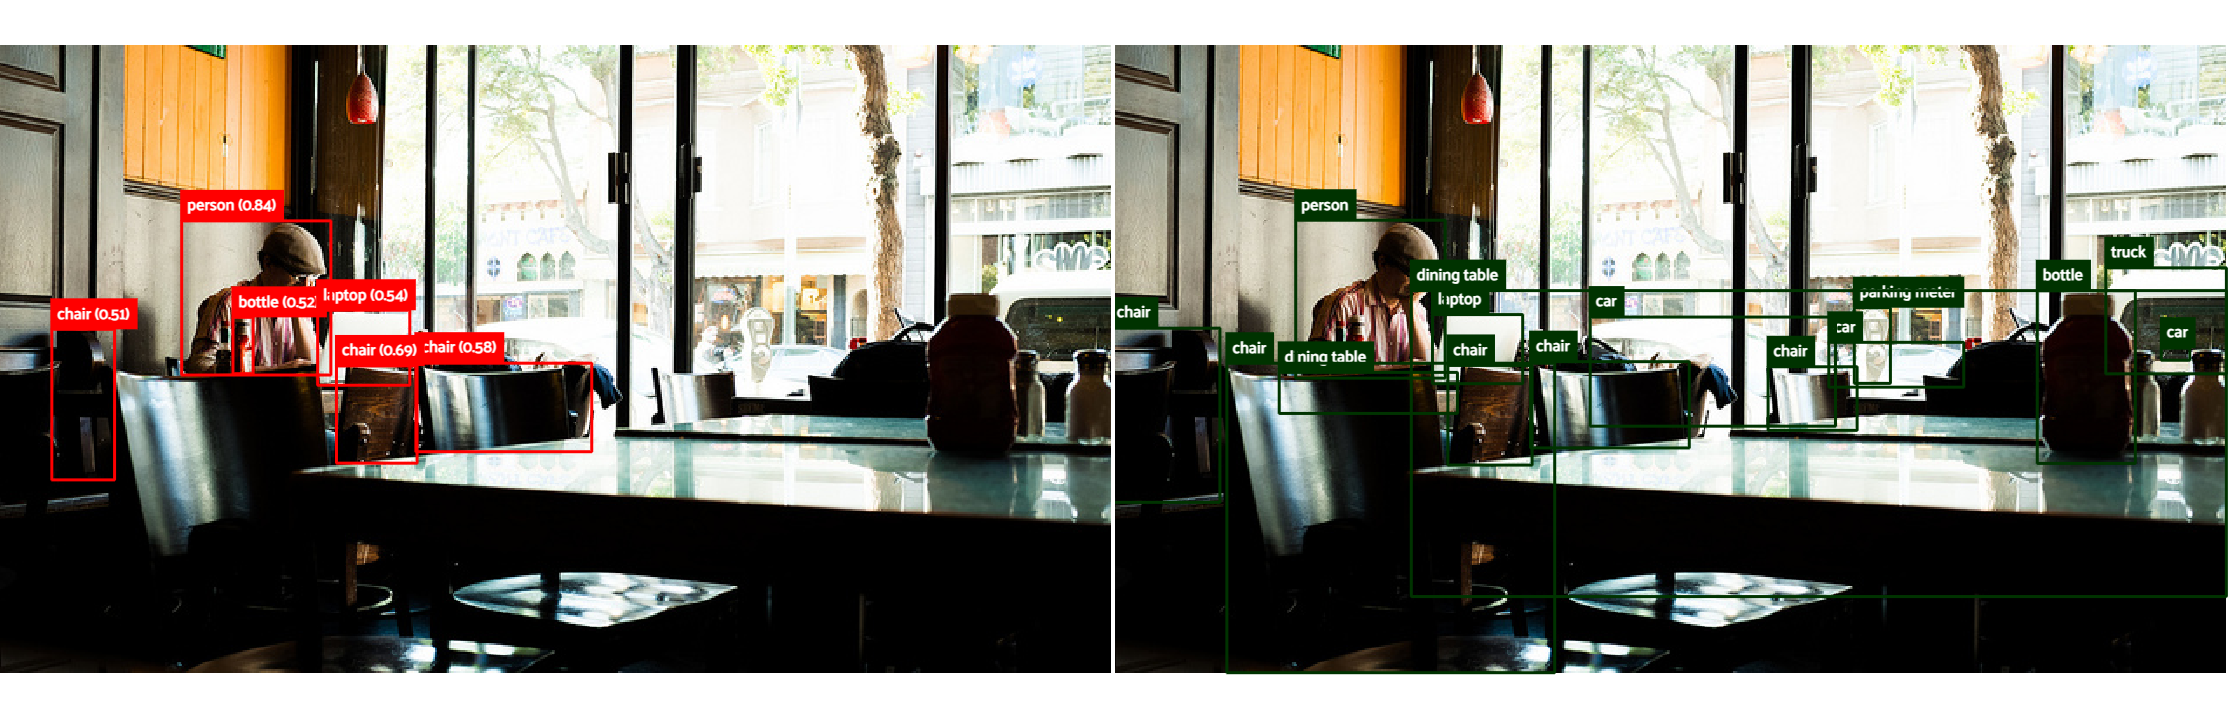
\includegraphics[width=0.5\textwidth]{images/retina_res/retina_w3.png}}
    {\raggedleft
    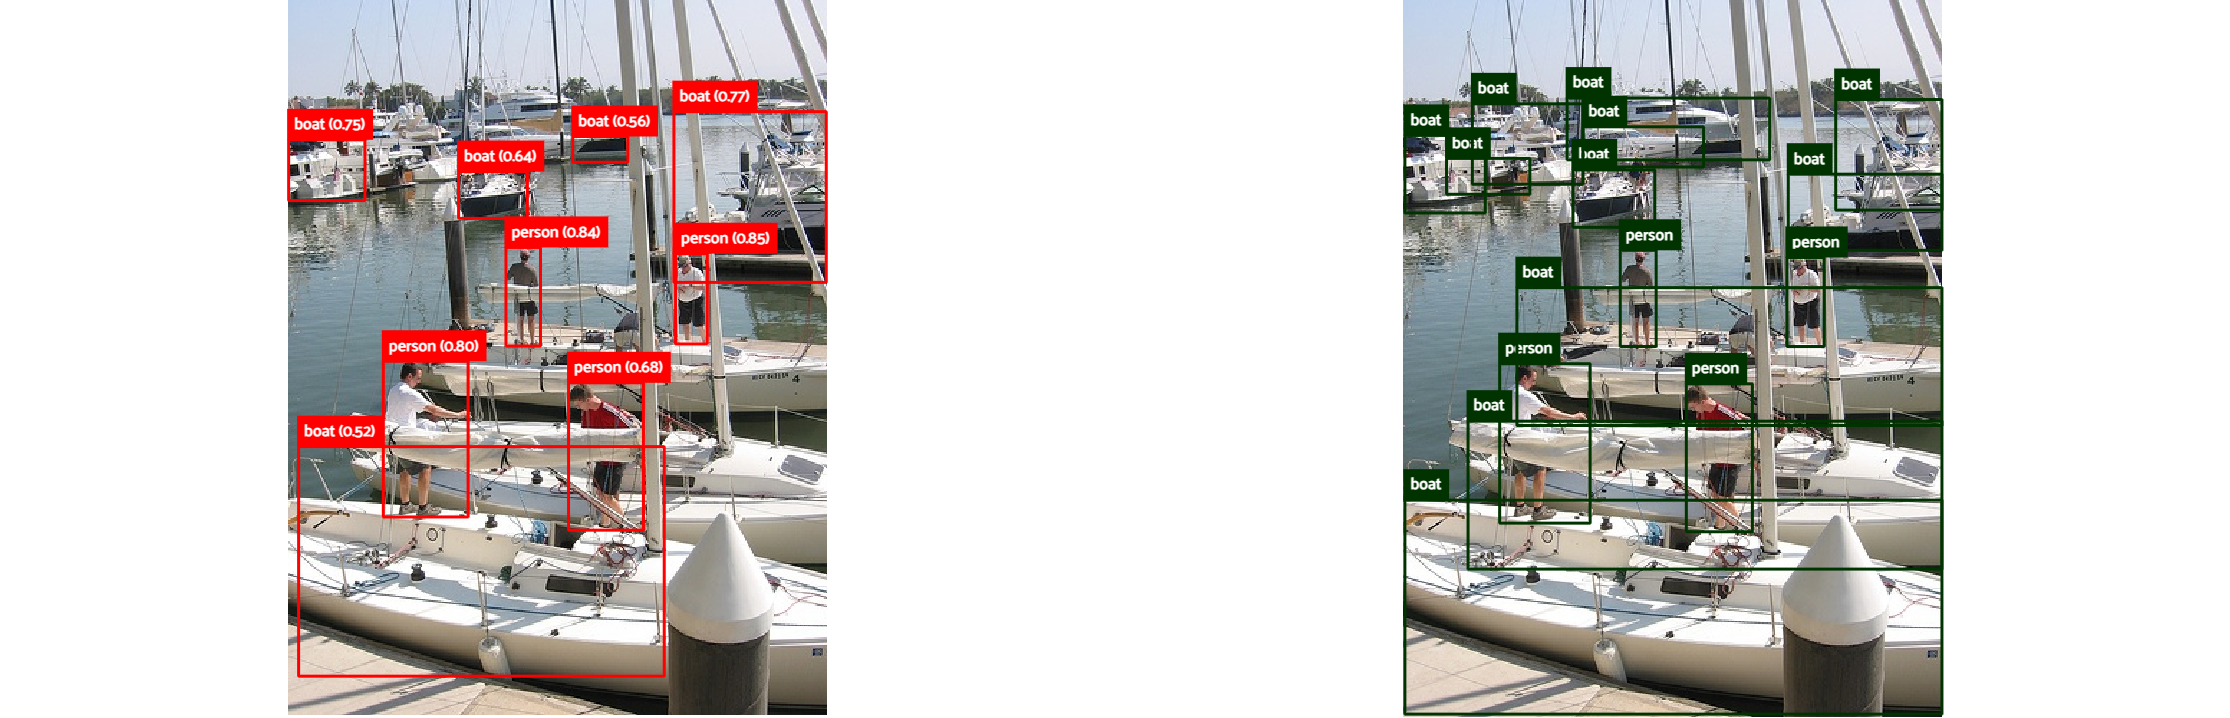
\includegraphics[width=0.5\textwidth]{images/retina_res/retina_w4.png}
    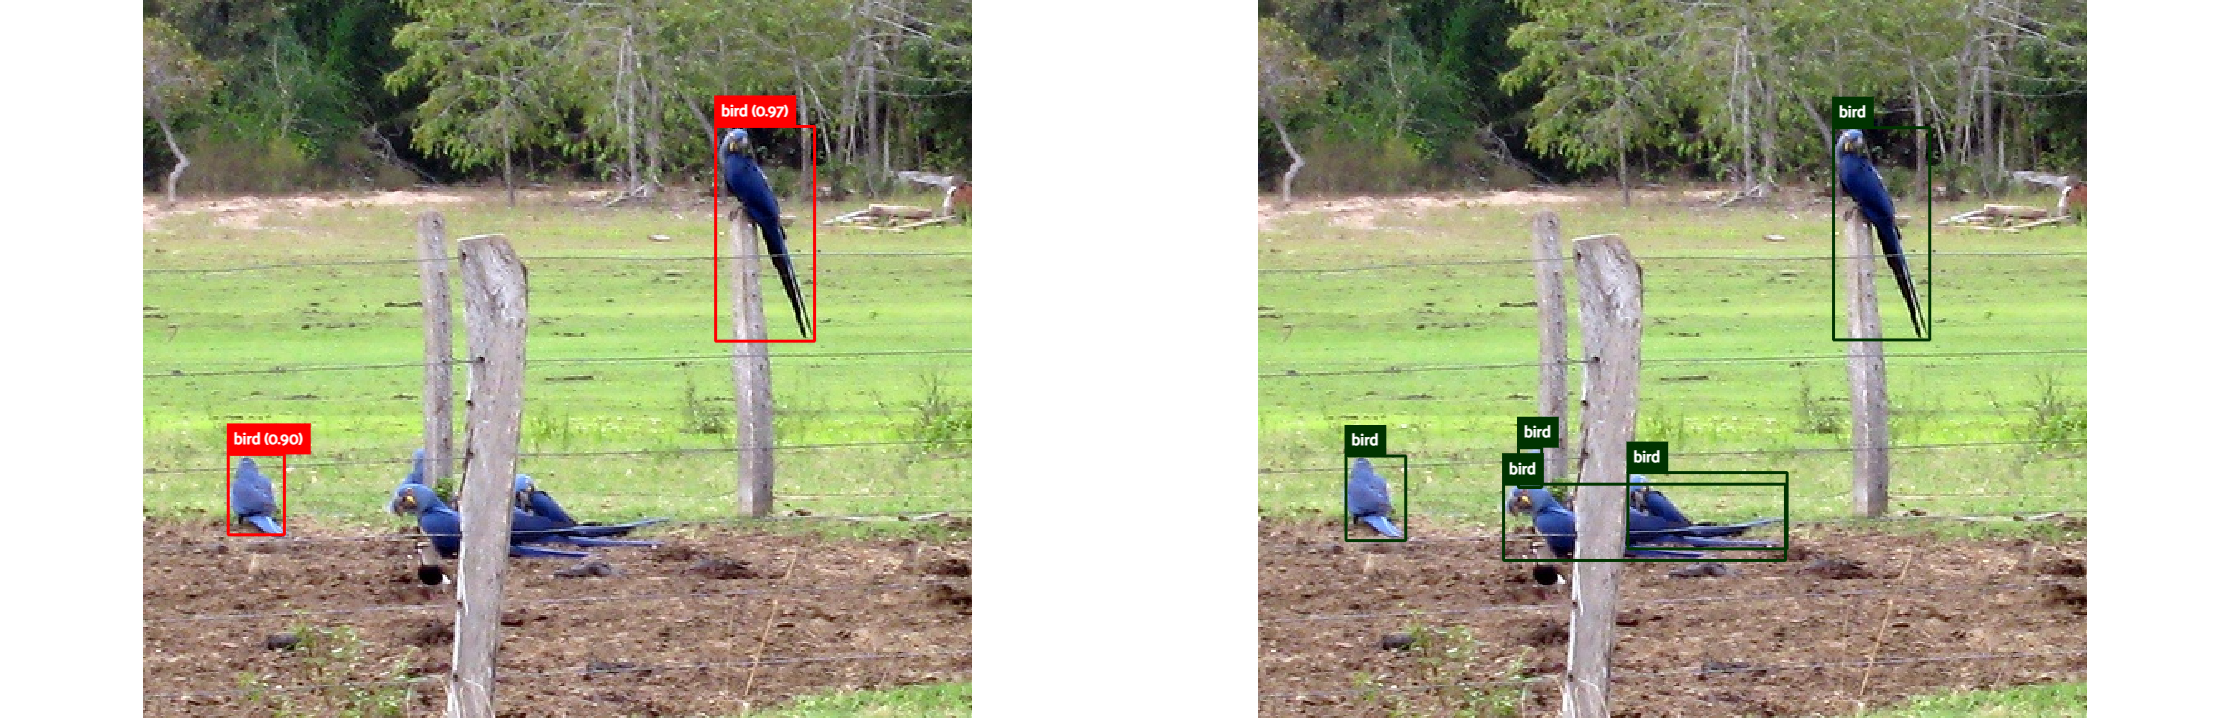
\includegraphics[width=0.5\textwidth]{images/retina_res/retina_w5.png}
    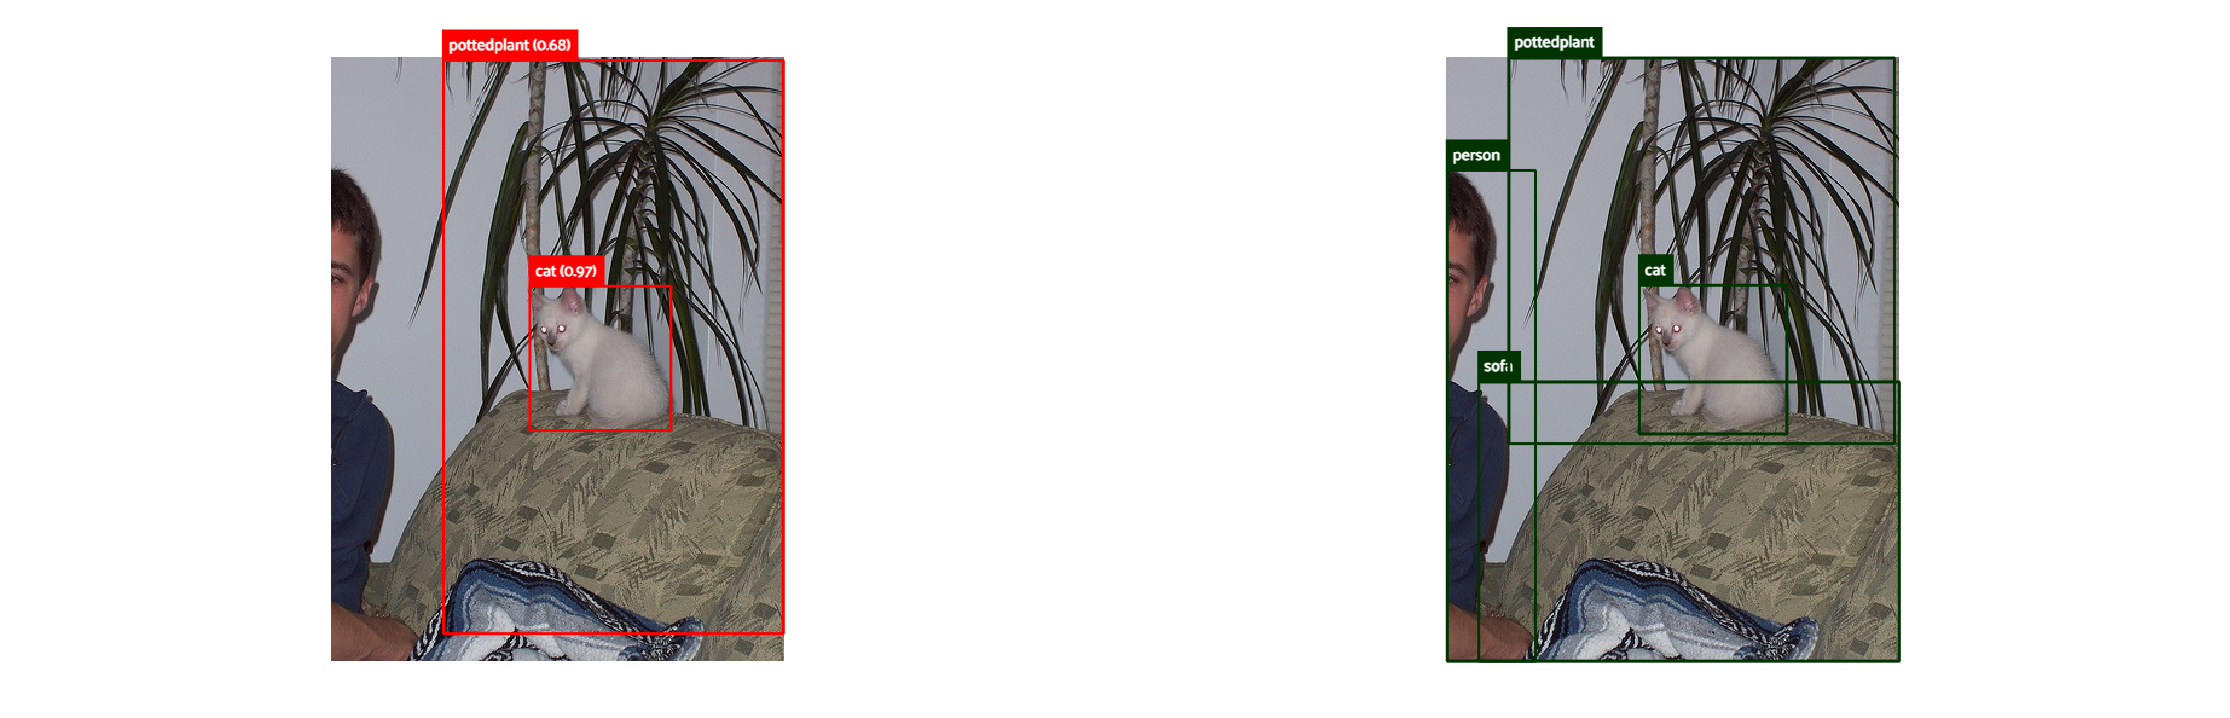
\includegraphics[width=0.5\textwidth]{images/retina_res/retina_w6.png}}
    \caption{Retina Net Worst Predictions}
    \label{fig:retina3}
\end{figure}

Best predictions is at Figure \ref{fig:retina2}.
\\
Worst predictions is at Figure \ref{fig:retina3}.
\newpage
\section{Models Comparison}
\begin{table}[h]
    \centering
    \begin{tabular}{|c|c|c|c|}
    \hline
    Metric & SSD & Faster R-CNN & Retina Net \\ \hline
    mAP & 0.225 & 0.367 & 0.357 \\ \hline
    IoU & 0.810 & 0.856 & 0.873 \\ \hline
    \end{tabular}
    \caption{COCO Scores}
    \label{table1}
\end{table}

\begin{table}[h]
    \centering
    \begin{tabular}{|c|c|c|c|}
    \hline
    Metric & SSD & Faster R-CNN & Retina Net \\ \hline
    mAP & 0.469 & 0.522 & 0.554 \\ \hline
    IoU &  0.819 & 0.815 & 0.829 \\ \hline
    \end{tabular}
    \caption{Pascal Scores}
    \label{table2}
\end{table}
\subsection{SSD}
\paragraph{Advantages:}
\begin{enumerate}[leftmargin=1cm, labelwidth=4cm]
  \item Speed: SSD is faster than the multi-stage detectors because it makes predictions at single pass making it well-suited for real-time applications
  \item Simple Architecture: Making it fast to train and deploy.
  \item Detect objects at different scales: makes use of multi-scale features and default boxes.
  \item Using the pretrained backbone: can take advantage of the large labeled data available for the image classification network, which makes it possible to train on a small dataset.
\end{enumerate}

\paragraph{Disadvantages:}
\begin{enumerate}[leftmargin=1cm, labelwidth=4cm]
  \item Lower Accuracy: Although the model has better speed, it suffers from low accuracy due to decreasing the resolution of the image at low quality and cannot take advantage of the additional context and information that multi-stage model provide
  \item Small-Scale Objects and Localization: The model struggles to detect small objects and has lower localization than the multi-stage models.
\end{enumerate}

\subsection{Faster R-CNN}
\paragraph{Advantages:}
\begin{enumerate}[leftmargin=1cm, labelwidth=4cm]
  \item High Accuracy: Faster R-CNN typically achieves higher accuracy in object detection tasks compared to its predecessors. 
  It utilizes a region proposal network (RPN) to generate potential object regions, which helps in accurate localization.
  \item Region Proposal Network (RPN): The introduction of RPN in Faster R-CNN allows the model to efficiently propose candidate object regions, eliminating the need for external region proposal methods. RPN shares features with the object detection network, making the model more streamlined.
  \item End-to-End Training: Faster R-CNN allows for end-to-end training, which means the entire network, including the region proposal network and the object detection network, can be trained together. This simplifies the training process and improves the overall performance of the model.
\end{enumerate}

\paragraph{Disadvantages:}
\begin{enumerate}[leftmargin=1cm, labelwidth=4cm]
  \item Computational Complexity: One of the main drawbacks of Faster R-CNN is its computational complexity.
  It can be slower during training and inference compared to some other object detection models.
The inclusion of the RPN adds an additional computational burden.
  \item Not Real-Time: While Faster R-CNN has been successful in many applications, it may not be suitable for real-time applications due to its computational demands.
\end{enumerate}

\subsection{Retina Net}
\paragraph{Advantages:}
\begin{enumerate}[leftmargin=1cm, labelwidth=4cm]
  \item Speed: It's faster than the R-CNN family and solved some of their issues resulting in higher accuracy. 
  \item Class Imbalance:  the cross-entropy loss in the previous models is replaced with the focal loss. The focal loss handles the class imbalance problems that exist in architectures like YOLO and SSD.
  \item Higher Accuracy:  It helps in combining the semantic rich features of lower resolution images with that of the semantically weak features of the higher resolution images using FPN resulted in better model performance.
  \item Aerial and Satellite imagery: The model can be used in satellite images due to its ability to detect small and dense objects.
\end{enumerate}

\paragraph{Disadvantages:}
\begin{enumerate}[leftmargin=1cm, labelwidth=4cm]
  \item Localization: Although the model achieved better accuracy it is not good in localization as R-CNN family which utilize regions to regress and make the bounding boxes more localized

\end{enumerate}

\end{document}
